\documentclass[12pt, a4paper, oneside]{article}
\usepackage[utf8]{vietnam}
\usepackage[utf8]{inputenc}
\usepackage[left=40mm, right=25mm, top=40mm, bottom=25mm]{geometry}
\usepackage{amsmath,amsfonts,amssymb}
\usepackage{indentfirst,enumitem}
\usepackage{graphicx}
\usepackage{multicol}
\usepackage{multirow}
\usepackage{setspace}
\usepackage{hyperref}
\usepackage{listings}
\usepackage{tabularx}
\usepackage{hyperref}
\usepackage{xcolor}
\usepackage{scrextend}
\usepackage{comment}
\usepackage{soul}
\usepackage{tipa}
\usepackage{subcaption}
\usepackage{caption}
\usepackage{booktabs}
\usepackage{array}
\usepackage{fancyhdr}
\usepackage{algorithm2e}
\usepackage{float}
\usepackage[most]{tcolorbox}
\usepackage{pdfpages}
\usepackage{import}
\usepackage{fancyhdr}
\usepackage[T5]{fontenc} % Hỗ trợ tiếng Việt
\usepackage{mathptmx} % Gói Times Roman
\graphicspath{ {figures/} }
\usepackage{titlesec}
\usepackage{tikz}
\usetikzlibrary{shapes.geometric, arrows, positioning, calc}
% Cấu hình Tiêu đề Chương (Section): Canh giữa, in hoa, đậm, cỡ 14
\titleformat{\section}[block]
  {\centering\normalfont\fontsize{14pt}{16.8pt}\bfseries\MakeUppercase}
  {\thesection}
  {0.5em}
  {}
% Cấu hình Tiêu đề Mục (Subsection): Đậm, chữ thường
\titleformat{\subsection}[hang]
  {\normalfont\normalsize\bfseries}
  {\thesubsection}
  {0.5em}
  {}

\captionsetup[table]{position=top, labelfont=bf, textfont=it, font=small, skip=5pt}
\captionsetup[figure]{position=bottom, labelfont=bf, textfont=it, font=small, skip=5pt}

\hypersetup{
    colorlinks=true,
    linkcolor=black,
    filecolor=magenta,      
    urlcolor=black,
    pdftitle={TKHTN},
    pdfpagemode=FullScreen,
}

\changefontsizes{13pt}
\renewcommand\thesection{\arabic{section}.}
\renewcommand\thesubsection{\arabic{section}.\arabic{subsection}}
\setlength{\parindent}{1.25cm}

\pagestyle{fancy}
\renewcommand{\headrulewidth}{0pt}
\fancyhf{} % Xóa cấu hình mặc định
\cfoot{\thepage} % Số trang ở giữa dưới (thường dùng)

\def\mathrlap{\mathpalette\mathrlapinternal} 
\def\mathclap{\mathpalette\mathclapinternal}
\def\mathllapinternal#1#2{\llap{$\mathsurround=0pt#1{#2}$}}
\def\mathrlapinternal#1#2{\rlap{$\mathsurround=0pt#1{#2}$}}

%CHÈN ẢNH
\usepackage{pgfplots}
\pgfplotsset{compat=1.15}
\usepackage{mathrsfs}
\usetikzlibrary{arrows}
\usetikzlibrary[patterns]

%New colors defined below
\definecolor{codegreen}{rgb}{0,0.6,0}
\definecolor{codegray}{rgb}{0.5,0.5,0.5}
\definecolor{codepurple}{rgb}{0.58,0,0.82}
\definecolor{backcolour}{rgb}{0.95,0.95,0.92}

%Code listing style named "mystyle"
\lstdefinestyle{mystyle}{
  backgroundcolor=\color{backcolour},   commentstyle=\color{codegreen},
  keywordstyle=\color{blue},
  numberstyle=\tiny\color{codegray},
  stringstyle=\color{codepurple},
  basicstyle=\ttfamily\footnotesize,
  breakatwhitespace=false,         
  breaklines=true,                 
  captionpos=b,                    
  keepspaces=true,                 
  numbers=left,                    
  numbersep=5pt,                  
  showspaces=false,                
  showstringspaces=false,
  showtabs=false,                  
  tabsize=2
}

%"mystyle" code listing set
\lstset{style=mystyle}

\begin{document}
\begin{titlepage}
%\SetWatermarkText{\includegraphics[width = 0.97\paperwidth,
%height = 0.97\paperheight]{bia.png}}
%\SetWatermarkAngle{0} 
%\SetWatermarkText{\includegraphics[scale=1]{hust.png}}
%\SetWatermarkAngle{0} 
\begin{tikzpicture}[remember picture,overlay,inner sep=0,outer sep=0]
     % Đã đổi xshift ở B và C từ 1.5cm thành 3cm để dịch khung sang phải né gáy sách 40mm
     \draw[blue!70!black,line width=4pt] ([xshift=-1.5cm,yshift=-2cm]current page.north east) coordinate (A)--([xshift=3cm,yshift=-2cm]current page.north west) coordinate(B)--([xshift=3cm,yshift=2cm]current page.south west) coordinate (C)--([xshift=-1.5cm,yshift=2cm]current page.south east) coordinate(D)--cycle;

     \draw ([yshift=0.5cm,xshift=-0.5cm]A)-- ([yshift=0.5cm,xshift=0.5cm]B)--
     ([yshift=-0.5cm,xshift=0.5cm]B) --([yshift=-0.5cm,xshift=-0.5cm]B)--([yshift=0.5cm,xshift=-0.5cm]C)--([yshift=0.5cm,xshift=0.5cm]C)--([yshift=-0.5cm,xshift=0.5cm]C)-- ([yshift=-0.5cm,xshift=-0.5cm]D)--([yshift=0.5cm,xshift=-0.5cm]D)--([yshift=0.5cm,xshift=0.5cm]D)--([yshift=-0.5cm,xshift=0.5cm]A)--([yshift=-0.5cm,xshift=-0.5cm]A)--([yshift=0.5cm,xshift=-0.5cm]A);

     \draw ([yshift=-0.3cm,xshift=0.3cm]A)-- ([yshift=-0.3cm,xshift=-0.3cm]B)--
     ([yshift=0.3cm,xshift=-0.3cm]B) --([yshift=0.3cm,xshift=0.3cm]B)--([yshift=-0.3cm,xshift=0.3cm]C)--([yshift=-0.3cm,xshift=-0.3cm]C)--([yshift=0.3cm,xshift=-0.3cm]C)-- ([yshift=0.3cm,xshift=0.3cm]D)--([yshift=-0.3cm,xshift=0.3cm]D)--([yshift=-0.3cm,xshift=-0.3cm]D)--([yshift=0.3cm,xshift=-0.3cm]A)--([yshift=0.3cm,xshift=0.3cm]A)--([yshift=-0.3cm,xshift=0.3cm]A);
\end{tikzpicture}
\begin{center}
    \vspace{7pt}
        \textbf{ĐẠI HỌC QUỐC GIA THÀNH PHỐ HỒ CHÍ MINH}
    
    \vspace{7pt}
    {TRƯỜNG ĐẠI HỌC BÁCH KHOA}
    
    \vspace{7pt}
    {KHOA ĐIỆN - ĐIỆN TỬ}

\end{center}
\vspace{10pt}
\begin{center}
    
\includegraphics[scale=0.3]{HCMUT.png}
    
    \vspace{10pt}
\end{center}

\begin{center}
    \fontsize{18pt}{17pt}\selectfont 
    \textbf{ĐỒ ÁN MÔN HỌC 1 (EE3183)}
\end{center}
\begin{center}
    \fontsize{15pt}{17pt}\selectfont 
    \textbf{\textrm{ĐỀ TÀI: THIẾT KẾ HỘP THUỐC THÔNG MINH IOT - 
    \\
    IOT SMART PILLBOX}}
\end{center}

\begin{center}
    \vspace{15pt}
% \textbf{Lớp: L03 - NHÓM: 5}
\end{center}

\vspace{10pt}

\begin{table}[h]
\begin{tabular}{rrl}
\hspace{6 cm} & SVTH: &Nguyễn Minh Thuận\\
& MSSV: &2313355\\
& GVHD: &TS. Nguyễn Thanh Tuấn
\end{tabular}
\end{table}
\vfill
\centerline{\bf Thành phố Hồ Chí Minh, tháng 6 năm 2026}

\vspace{1cm}
\end{titlepage}

\newpage

\newpage
\thispagestyle{empty}
\setstretch{1.3}
\begin{center}
    \textbf{LỜI CẢM ƠN}
\end{center}

\textit{Em xin gửi lời cảm ơn chân thành và sự tri ân sâu sắc đối với thầy Nguyễn Thanh Tuấn, giảng viên Bộ môn Viễn Thông, Khoa Điện - Điện tử, Trường Đại học Bách khoa - Đại học Quốc gia Thành phố Hồ Chí Minh, đã tạo điều kiện cho em có thể hoàn thành được học phần Đồ Án 1 này. Và em cũng xin chân thành cảm ơn thầy đã nhiệt tình hướng dẫn, chỉ ra những điều còn thiếu sót trong qua trình thực hiện đề tài để có được kết quả tốt đẹp như mong muốn và hoàn thành tốt học phần này.}

\textit{Trong quá trình thực hiện đề tài, thầy đã chỉ dẫn, góp ý và giúp em khắc phục những thiếu sót để đạt được kết quả tốt hơn. Do hạn chế về kiến thức và kinh nghiệm thực tiễn, bài báo cáo không thể tránh khỏi những sai sót. Em rất mong nhận được sự thông cảm và những ý kiến đóng góp quý báu từ thầy để có thể hoàn thiện hơn trong các học phần tiếp theo cũng như trong đồ án và luận văn tốt nghiệp sau này.}

\textit{Em xin chân thành cảm ơn Thầy!}

\textit{Chúc Thầy sức khỏe và thành đạt.}

\vspace{4cm}

\hspace{5cm}\textit{Tp. Hồ Chí Minh, ngày .... tháng .... năm ........}

\hspace{8cm}\textbf{Sinh viên}

\newpage
\thispagestyle{empty}
\setstretch{1.3}
\begin{center}
    \textbf{TÓM TẮT ĐỀ TÀI}
\end{center}

Tuân thủ phác đồ điều trị và uống thuốc đúng giờ là yếu tố tiên quyết quyết định hiệu quả của quá trình chăm sóc y tế, đặc biệt đối với người cao tuổi và bệnh nhân mắc các bệnh mãn tính. Tuy nhiên, tình trạng quên uống thuốc, uống sai cữ hoặc bỏ liều vẫn thường xuyên diễn ra do sự suy giảm trí nhớ hoặc nhịp sống bận rộn. Nhằm giải quyết triệt để vấn đề này, đề tài "Thiết kế hộp thuốc thông minh IoT - IoT Smart Pillbox" được triển khai với mục tiêu xây dựng một hệ sinh thái hỗ trợ quản lý y tế cá nhân khép kín, tự động và theo thời gian thực. 

Cốt lõi của hệ thống được phát triển dựa trên vi điều khiển trung tâm ESP32, kết hợp cùng công tắc hành trình để giám sát chính xác các thao tác vật lý, màn hình OLED 0.96 inch để giao tiếp trực quan và còi báo chủ động nhằm tạo ra chu trình nhắc nhở hiệu quả. Thiết bị đảm bảo tính di động và vận hành liên tục nhờ cơ chế cấp nguồn linh hoạt qua cổng USB Type-C hoặc hệ thống pin Lithium-ion đi kèm mạch quản lý năng lượng. 

Điểm đột phá của đề tài nằm ở việc ứng dụng kiến trúc điện toán phi máy chủ (Serverless) thay cho các máy chủ trung gian truyền thống, sử dụng Google Apps Script làm nền tảng Backend và Google Sheets làm cơ sở dữ liệu. Nhờ triển khai các thuật toán xử lý đa nhiệm không đồng bộ (non-blocking) trên vi điều khiển, thiết bị có khả năng đánh giá và phân loại chính xác các trạng thái phức tạp như "Đã uống", "Bỏ thuốc" hay "Uống trễ". Toàn bộ dữ liệu được đồng bộ hóa với một trang quản trị trực tuyến (Web Dashboard), cho phép người nhà hoặc bác sĩ dễ dàng thiết lập lịch trình từ xa, tra cứu nhật ký y tế và nhận thông báo cảnh báo tức thời qua ứng dụng Telegram. 

Kết quả thực nghiệm khẳng định hệ thống vận hành ổn định, độ trễ truyền tải thấp và logic xử lý đáp ứng trọn vẹn các kịch bản thực tế, qua đó mở ra tiềm năng ứng dụng mạnh mẽ cho các thiết bị y tế thông minh phân tán trong tương lai.

\newpage
\thispagestyle{empty}
\setstretch{1.3}
\renewcommand{\contentsname}{\centering {MỤC LỤC}}
\tableofcontents



\newpage
\setcounter{page}{1}

\begin{center}
    \section{GIỚI THIỆU}
\end{center}
\subsection{Tổng quan}
%Nội dung 1.1
Sự phát triển bùng nổ của Internet vạn vật (IoT) đã và đang tạo ra những bước nhảy vọt trong lĩnh vực y tế số (Digital Health). Xu hướng chuyển dịch từ việc chăm sóc sức khỏe tập trung tại bệnh viện sang giám sát cá nhân hóa tại gia đình đang ngày càng trở nên phổ biến. Trong bối cảnh đó, vấn đề tuân thủ thời gian biểu sử dụng thuốc (Medication Adherence) nổi lên như một thách thức lớn. Theo nhiều báo cáo y khoa, việc người bệnh (đặc biệt là người cao tuổi, người suy giảm trí nhớ) quên uống thuốc, uống quá liều hoặc sai cữ không chỉ làm vô hiệu hóa phác đồ điều trị mà còn gây ra những biến chứng nguy hiểm, gia tăng gánh nặng cho hệ thống y tế.

Xuất phát từ nhu cầu thực tiễn cấp thiết đó, đề tài "Thiết kế hộp thuốc thông minh IoT" được đề xuất và thực hiện. Không chỉ dừng lại ở một thiết bị phần cứng phát tiếng kêu báo thức đơn thuần, đề tài hướng tới việc xây dựng một hệ thống quản lý dữ liệu y tế toàn diện. Sự kết hợp giữa vi điều khiển có kết nối Wi-Fi (ESP32) tại nơi người bệnh và sức mạnh xử lý của điện toán đám mây (Cloud Computing) tạo ra một luồng thông tin xuyên suốt. Người nhà hoặc bác sĩ có thể dễ dàng thiết lập phác đồ uống thuốc từ xa, trong khi hệ thống phần cứng sẽ tự động tương tác với bệnh nhân và gửi báo cáo hành vi chi tiết (đúng giờ, trễ giờ, bỏ cữ) theo thời gian thực về máy chủ.

\subsection{Tình hình nghiên cứu trong và ngoài nước}
%Nội dung 1.2
\subsubsection{Tình hình nghiên cứu ngoài nước:} 

Trên thị trường quốc tế, các sản phẩm hộp thuốc thông minh đã bắt đầu được thương mại hóa, tiêu biểu như các dòng sản phẩm của Ellie, Medisafe hay Hero. Các hệ thống này thường có thiết kế cơ khí tinh xảo, phân chia nhiều ngăn tự động. Về mặt công nghệ, chúng chủ yếu sử dụng giao thức Bluetooth (BLE) để đồng bộ dữ liệu với ứng dụng trên điện thoại thông minh (Smartphone) của người dùng, hoặc sử dụng Wi-Fi để kết nối với các máy chủ đám mây độc quyền (Proprietary Cloud). Nhược điểm chung của các giải pháp này là giá thành phần cứng rất cao, bắt buộc người dùng phải trả phí thuê bao (Subscription) hàng tháng để duy trì dịch vụ lưu trữ dữ liệu, và quá trình thiết lập ứng dụng đi kèm khá phức tạp đối với tệp người dùng là người cao tuổi.

\subsubsection{Tình hình nghiên cứu trong nước:} 

Tại Việt Nam, các nghiên cứu và sản phẩm ứng dụng IoT trong quản lý hộp thuốc chủ yếu xuất hiện dưới dạng các mô hình đồ án sinh viên hoặc sản phẩm khởi nghiệp quy mô nhỏ. Đa số các mô hình sử dụng vi điều khiển như Arduino Uno kết hợp module ESP8266, hoặc sử dụng cơ sở dữ liệu thời gian thực Firebase của Google. Dù giải quyết được bài toán chi phí, nhưng các mô hình này thường thiếu tính đồng bộ và độ tin cậy. Các hệ thống đa phần gặp giới hạn ở việc xử lý đa nhiệm (bị treo hệ thống khi chờ kết nối mạng), không có giao diện Web tổng quan (Dashboard) độc lập mà phụ thuộc vào các nền tảng có sẵn như Blynk, và chưa tối ưu hóa được thuật toán phân tích hành vi "uống trễ" của người bệnh.

Đề tài này được thực hiện nhằm khắc phục các nhược điểm trên, bằng cách tự chủ hoàn toàn giao diện Web, tận dụng kiến trúc API của Google Apps Script để miễn phí hóa khâu lưu trữ, và xây dựng một nền tảng phần mềm nhúng hoạt động ổn định không bị tắc nghẽn.

\subsection{Nhiệm vụ đề tài}
%Nội dung 1.3
Để đạt được các mục tiêu đã đề ra, đề tài tập trung giải quyết các nhiệm vụ trọng tâm sau:
\begin{itemize}
    \item \textbf{Thiết kế và thi công phần cứng:} Lựa chọn linh kiện và thiết kế sơ đồ mạch điện xung quanh vi điều khiển trung tâm ESP32. Tích hợp màn hình OLED I2C, còi báo động, công tắc hành trình dạng đòn bẩy nảy (Limit switch).
    \item \textbf{Phát triển phần mềm nhúng:} Lập trình ESP32 trên nền tảng C++ với thuật toán xử lý đa nhiệm theo thời gian thực sử dụng hàm \texttt{millis()}, loại bỏ hoàn toàn các hàm dừng (delay) gây treo hệ thống. Triển khai giao thức NTP để đồng bộ thời gian chuẩn xác và HTTPS để truyền/nhận dữ liệu bảo mật.
    \item \textbf{Thiết kế hệ thống Điện toán đám mây:} Xây dựng mã nguồn Google Apps Script (GAS) đóng vai trò làm máy chủ API, xử lý các yêu cầu GET/POST từ mạch ESP32 và định tuyến dữ liệu vào bảng tính Google Sheets để lưu trữ dài hạn.
    \item \textbf{Phát triển Giao diện Người dùng (UI/UX):} Thiết kế và lập trình một trang Web Dashboard (sử dụng HTML/CSS/JavaScript) cho phép thiết lập lịch báo thức đa dạng (theo thứ trong tuần) và hiển thị thống kê lịch sử trực quan. Tích hợp API của Telegram để khởi tạo Bot thông báo từ xa.
    \item \textbf{Thử nghiệm và đánh giá:} Cấu hình cơ chế khôi phục mạng nội bộ và tiến hành đánh giá độ ổn định của toàn bộ hệ thống dưới các điều kiện vận hành thực tế.
\end{itemize}

\newpage
\begin{center}
    \section{LÝ THUYẾT}
\end{center}
%Nội dung chương 2
\subsection{Vi điều khiển trung tâm ESP32 NodeMCU Devkit V1}
\subsubsection{Kiến trúc phần cứng vi xử lý}

ESP32 NodeMCU Devkit V1 là bo mạch phát triển mã nguồn mở, được thiết kế tích hợp module hệ thống trên chip (SoC) ESP32-WROOM-32 do hãng Espressif Systems sản xuất.

Trái tim của hệ thống là bộ vi xử lý Xtensa® Dual-Core 32-bit LX6. Khác với các dòng vi điều khiển lõi đơn truyền thống như ATmega328P, kiến trúc lõi kép của ESP32 mang lại khả năng xử lý bất đối xứng trên nền tảng hệ điều hành thời gian thực FreeRTOS.

\begin{itemize}
    \item \textit{ Lõi PRO\_CPU}: Chuyên trách xử lý các luồng tác vụ ngầm ở tầng thấp như ngăn xếp giao thức Wi-Fi, Bluetooth và quản lý các ngắt phần cứng cường độ cao.
    \item \textit{Lõi APP\_CPU}: Được giải phóng hoàn toàn để thực thi mã chương trình của người dùng (logic giám sát hành trình nắp hộp, xuất tín hiệu âm thanh và cập nhật màn hình OLED). 
    Hệ thống sử dụng đường dẫn dữ liệu (Data bus) và đường dẫn lệnh (Instruction bus) độc lập theo kiến trúc Harvard, mang lại khả năng tính toán lên đến 600 DMIPS, đáp ứng hoàn hảo yêu cầu phân tích (parsing) các chuỗi dữ liệu JSON phức tạp tải về từ máy chủ đám mây.
\end{itemize}

\begin{figure}
    \centering
    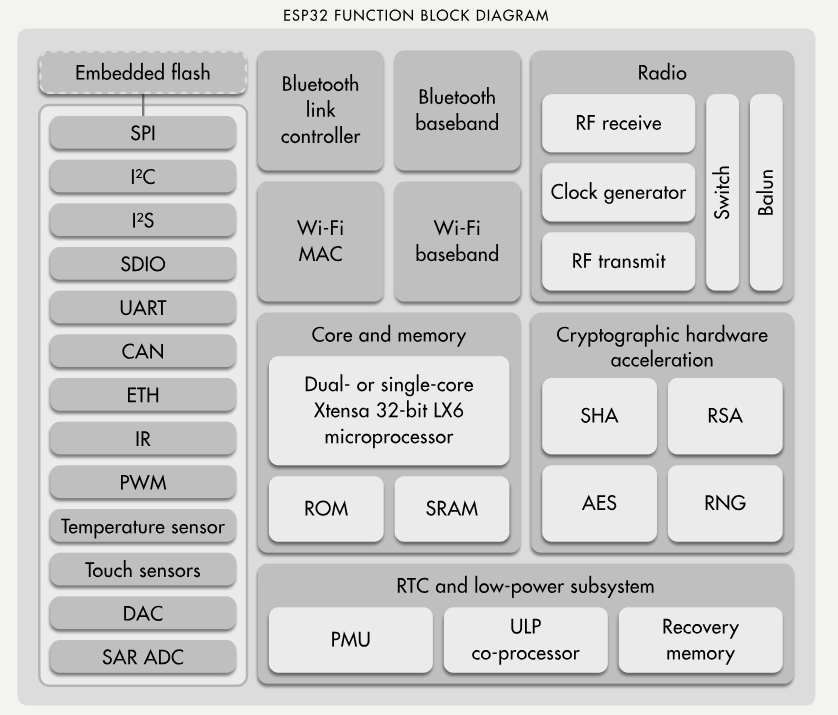
\includegraphics[width=0.8\textwidth]{ESP32 FUNCTION BLOCK DIAGRAM.png}
    \caption{Sơ đồ khối chức năng của ESP32}
    \label{fig:espblockdiagram}
\end{figure}

\newpage
\subsubsection{Thông số kỹ thuật chi tiết và Ngoại vi}

Dựa trên tài liệu kỹ thuật của nhà sản xuất, SoC ESP32-WROOM-32 sở hữu các thông số phần cứng vượt trội, đáp ứng tiêu chuẩn của một thiết bị IoT công nghiệp:

\begin{itemize}
    \item Hệ thống Nguồn điện: Điện áp hoạt động lõi của chip là $2.2V - 3.6V$. Tuy nhiên, trên mạch Devkit V1 đã được tích hợp sẵn IC ổn áp tuyến tính như AMS1117-3.3, cho phép cấp nguồn $5V$ an toàn qua cổng Micro-USB hoặc chân VIN. Chip được trang bị bộ xử lý đồng xử lý siêu tiết kiệm năng lượng (ULP), cho phép dòng tiêu thụ giảm xuống mức cực thấp (khoảng $10 \mu A$) ở chế độ Ngủ sâu (Deep-sleep), rất lý tưởng cho các thiết bị y tế chạy pin.
    \item Hệ thống Bộ nhớ: Tích hợp sẵn $520 KB$ SRAM nội bộ và $448 KB$ ROM. Ngoài ra, module WROOM-32 được gắn kèm một chip nhớ Flash SPI ngoại vi dung lượng $4MB$ (hoặc $8MB$ tùy phiên bản), cung cấp không gian rộng rãi để lưu trữ Firmware, hệ thống tệp tĩnh (SPIFFS) và cơ sở dữ liệu nội bộ.
    \item Giao tiếp Ngoại vi (I/O Interfaces): Mạch cung cấp tổng cộng 34 chân GPIO với khả năng ghép kênh linh hoạt bằng phần mềm.
    \begin{itemize}
        \item Giao tiếp số: Hỗ trợ phần cứng chuyên dụng cho 3 x UART, 3 x SPI, 2 x I2C và 2 x I2S
        \item Giao tiếp tương tự: Tích hợp bộ chuyển đổi tương tự - số (ADC) kiến trúc SAR 12-bit với 18 kênh; và bộ chuyển đổi số - tương tự (DAC) 8-bit với 2 kênh.
        \item Cảm biến tích hợp: Chip tích hợp sẵn cảm biến hiệu ứng Hall (đo từ trường) và 10 chân GPIO hỗ trợ cảm biến điện dung, cho phép thiết kế các nút bấm không tiếp xúc cơ học.
    \end{itemize}
\end{itemize}
\subsubsection{Khả năng vô tuyến: Wi-Fi và Bluetooth}
Khả năng tích hợp RF trên ESP32 là một bước tiến lớn trong thiết kế bán dẫn, bao gồm bộ thu phát vô tuyến, bộ khuếch đại nhiễu thấp (LNA), bộ khuếch đại công suất (PA) và bộ chuyển mạch ăng-ten (Antenna switch) được nhúng gọn trong cùng một đế silicon (kích thước chỉ $18mm \times 25.5mm$).

\begin{itemize}
    \item Tầng Vật lý Wi-Fi: Tuân thủ chuẩn IEEE 802.11 b/g/n, hoạt động ở băng tần $2.4 GHz$ ISM. ESP32 hỗ trợ cấu trúc liên kết mạng linh hoạt: chế độ Station (thiết bị đầu cuối kết nối vào Router), SoftAP (tự phát mạng nội bộ) và kết hợp BSS. Với công suất phát định mức lên đến $+19.5 dBm$ (chuẩn 802.11b) và độ nhạy thu (RX Sensitivity) đạt $-97 dBm$, thiết bị đảm bảo duy trì liên kết vô tuyến ổn định, khắc phục hiện tượng suy hao tín hiệu khi hộp thuốc đặt trong phòng kín hoặc vùng có vật cản.
    \item Kết nối Bluetooth: Tích hợp bộ điều khiển băng tần cơ sở hỗ trợ chuẩn Bluetooth v4.2 BR/EDR và đặc biệt là Bluetooth Low Energy (BLE). Trong kiến trúc IoT hiện đại, BLE mở ra hướng phát triển cho việc cấu hình mạng cục bộ hoặc giao tiếp trực tiếp với các thiết bị đeo tay thông minh của người bệnh để đồng bộ nhịp tim và nhắc nhở uống thuốc mà không cần thông qua Internet.
\end{itemize}
\subsection{Nền tảng Giao thức Mạng và Đồng bộ hệ thống}

Để hiện thực hóa kiến trúc Internet vạn vật (IoT), hệ thống không giới hạn ở tầng vật lý mà đòi hỏi việc thực thi các ngăn xếp giao thức (Protocol Stack) chuẩn mực trên nền tảng TCP/IP, đảm bảo tính bảo mật và độ chính xác thời gian tuyệt đối.

\subsubsection{Giao thức HTTPS (Hypertext Transfer Protocol Secure)}

Trong đề tài này, ESP32 tương tác trực tiếp với hệ sinh thái máy chủ đám mây của Google (Google Apps Script) mà không qua bất kỳ Broker trung gian nào. Do tính chất dữ liệu y tế cần độ bảo mật cao, giao thức HTTPS được áp dụng tại tầng Ứng dụng (Application Layer).

HTTPS là phần mở rộng bảo mật của giao thức HTTP, hoạt động qua cổng 443. Khác với giao thức HTTP truyền văn bản gốc (plaintext) dễ bị tấn công nghe lén (Packet Sniffing), HTTPS thiết lập một đường hầm bảo mật bằng giao thức TLS/SSL (Transport Layer Security).

\begin{itemize}
    \item Quá trình Handshake: ESP32 và máy chủ Google trao đổi thông tin để thống nhất bộ thuật toán mã hóa (Cipher Suite).
    \item Mã hóa phi đối xứng: Sử dụng các thuật toán như RSA hay ECC để trao đổi khóa phiên một cách an toàn.
    \item Mã hóa đối xứng: Sau khi có khóa phiên, toàn bộ dữ liệu tải trọng (Payload) – bao gồm lệnh Mo\_Nap hay chuỗi lịch sử báo thức – đều được mã hóa bằng AES-256.
    
    Đặc tính kỹ thuật trên ESP32: Quá trình xác thực chứng chỉ số tốn rất nhiều tài nguyên RAM. Để tối ưu hóa giới hạn bộ nhớ của vi điều khiển, thư viện \texttt{WiFiClientSecure} được cấu hình ở chế độ \texttt{setInsecure()}. Kỹ thuật này bỏ qua việc kiểm tra tính hợp lệ của chuỗi chứng chỉ máy chủ nhưng vẫn duy trì kênh mã hóa dữ liệu đầu cuối, đảm bảo cân bằng giữa bài toán bảo mật và hiệu năng phần cứng nhúng.
\end{itemize}

\subsubsection{Giao thức đồng bộ thời gian mạng NTP (Network Time Protocol)}

Tính năng cốt lõi của "Hộp thuốc thông minh" là báo thức chính xác. Do ESP32 không được trang bị mạch đồng hồ thời gian thực (RTC) chạy pin CMOS độc lập, việc lấy giờ chuẩn được phó thác hoàn toàn cho giao thức NTP.

NTP hoạt động trên nền tảng giao thức phi kết nối UDP (User Datagram Protocol) tại cổng 123. Nó được thiết kế để đồng bộ hóa đồng hồ của các hệ thống máy tính với các nguồn thời gian chuẩn toàn cầu (Stratum 1, Stratum 2).

Thuật toán cốt lõi của NTP không chỉ đơn thuần là "hỏi giờ". Khi ESP32 gửi gói tin yêu cầu đến máy chủ (ví dụ \texttt{pool.ntp.org}), thuật toán sẽ ghi nhận 4 dấu thời gian (timestamps): thời điểm đi, thời điểm máy chủ nhận, thời điểm máy chủ phản hồi và thời điểm ESP32 nhận lại. Dựa vào 4 biến số này, ngăn xếp giao thức sẽ tính toán được:

\begin{itemize}
    \item Độ trễ đường truyền (Network Delay): Tổng thời gian gói tin di chuyển trên không gian mạng.
    \item Độ lệch đồng hồ (Clock Offset): Sự chênh lệch thời gian thực tế giữa hệ thống dao động thạch anh nội bộ của ESP32 và đồng hồ nguyên tử của máy chủ.
    
Bằng cách bù trừ các sai số này, giao thức NTP cung cấp cho hộp thuốc một mốc thời gian (Epoch time) với sai số chỉ ở mức mili-giây, đảm bảo cữ thuốc được nhắc nhở chính xác theo thời gian thực tại múi giờ địa phương (GMT+7).
\end{itemize}

\subsection{Màn hình OLED 0.96 inch và Giao thức I2C}

\begin{figure}[H]
    \centering
    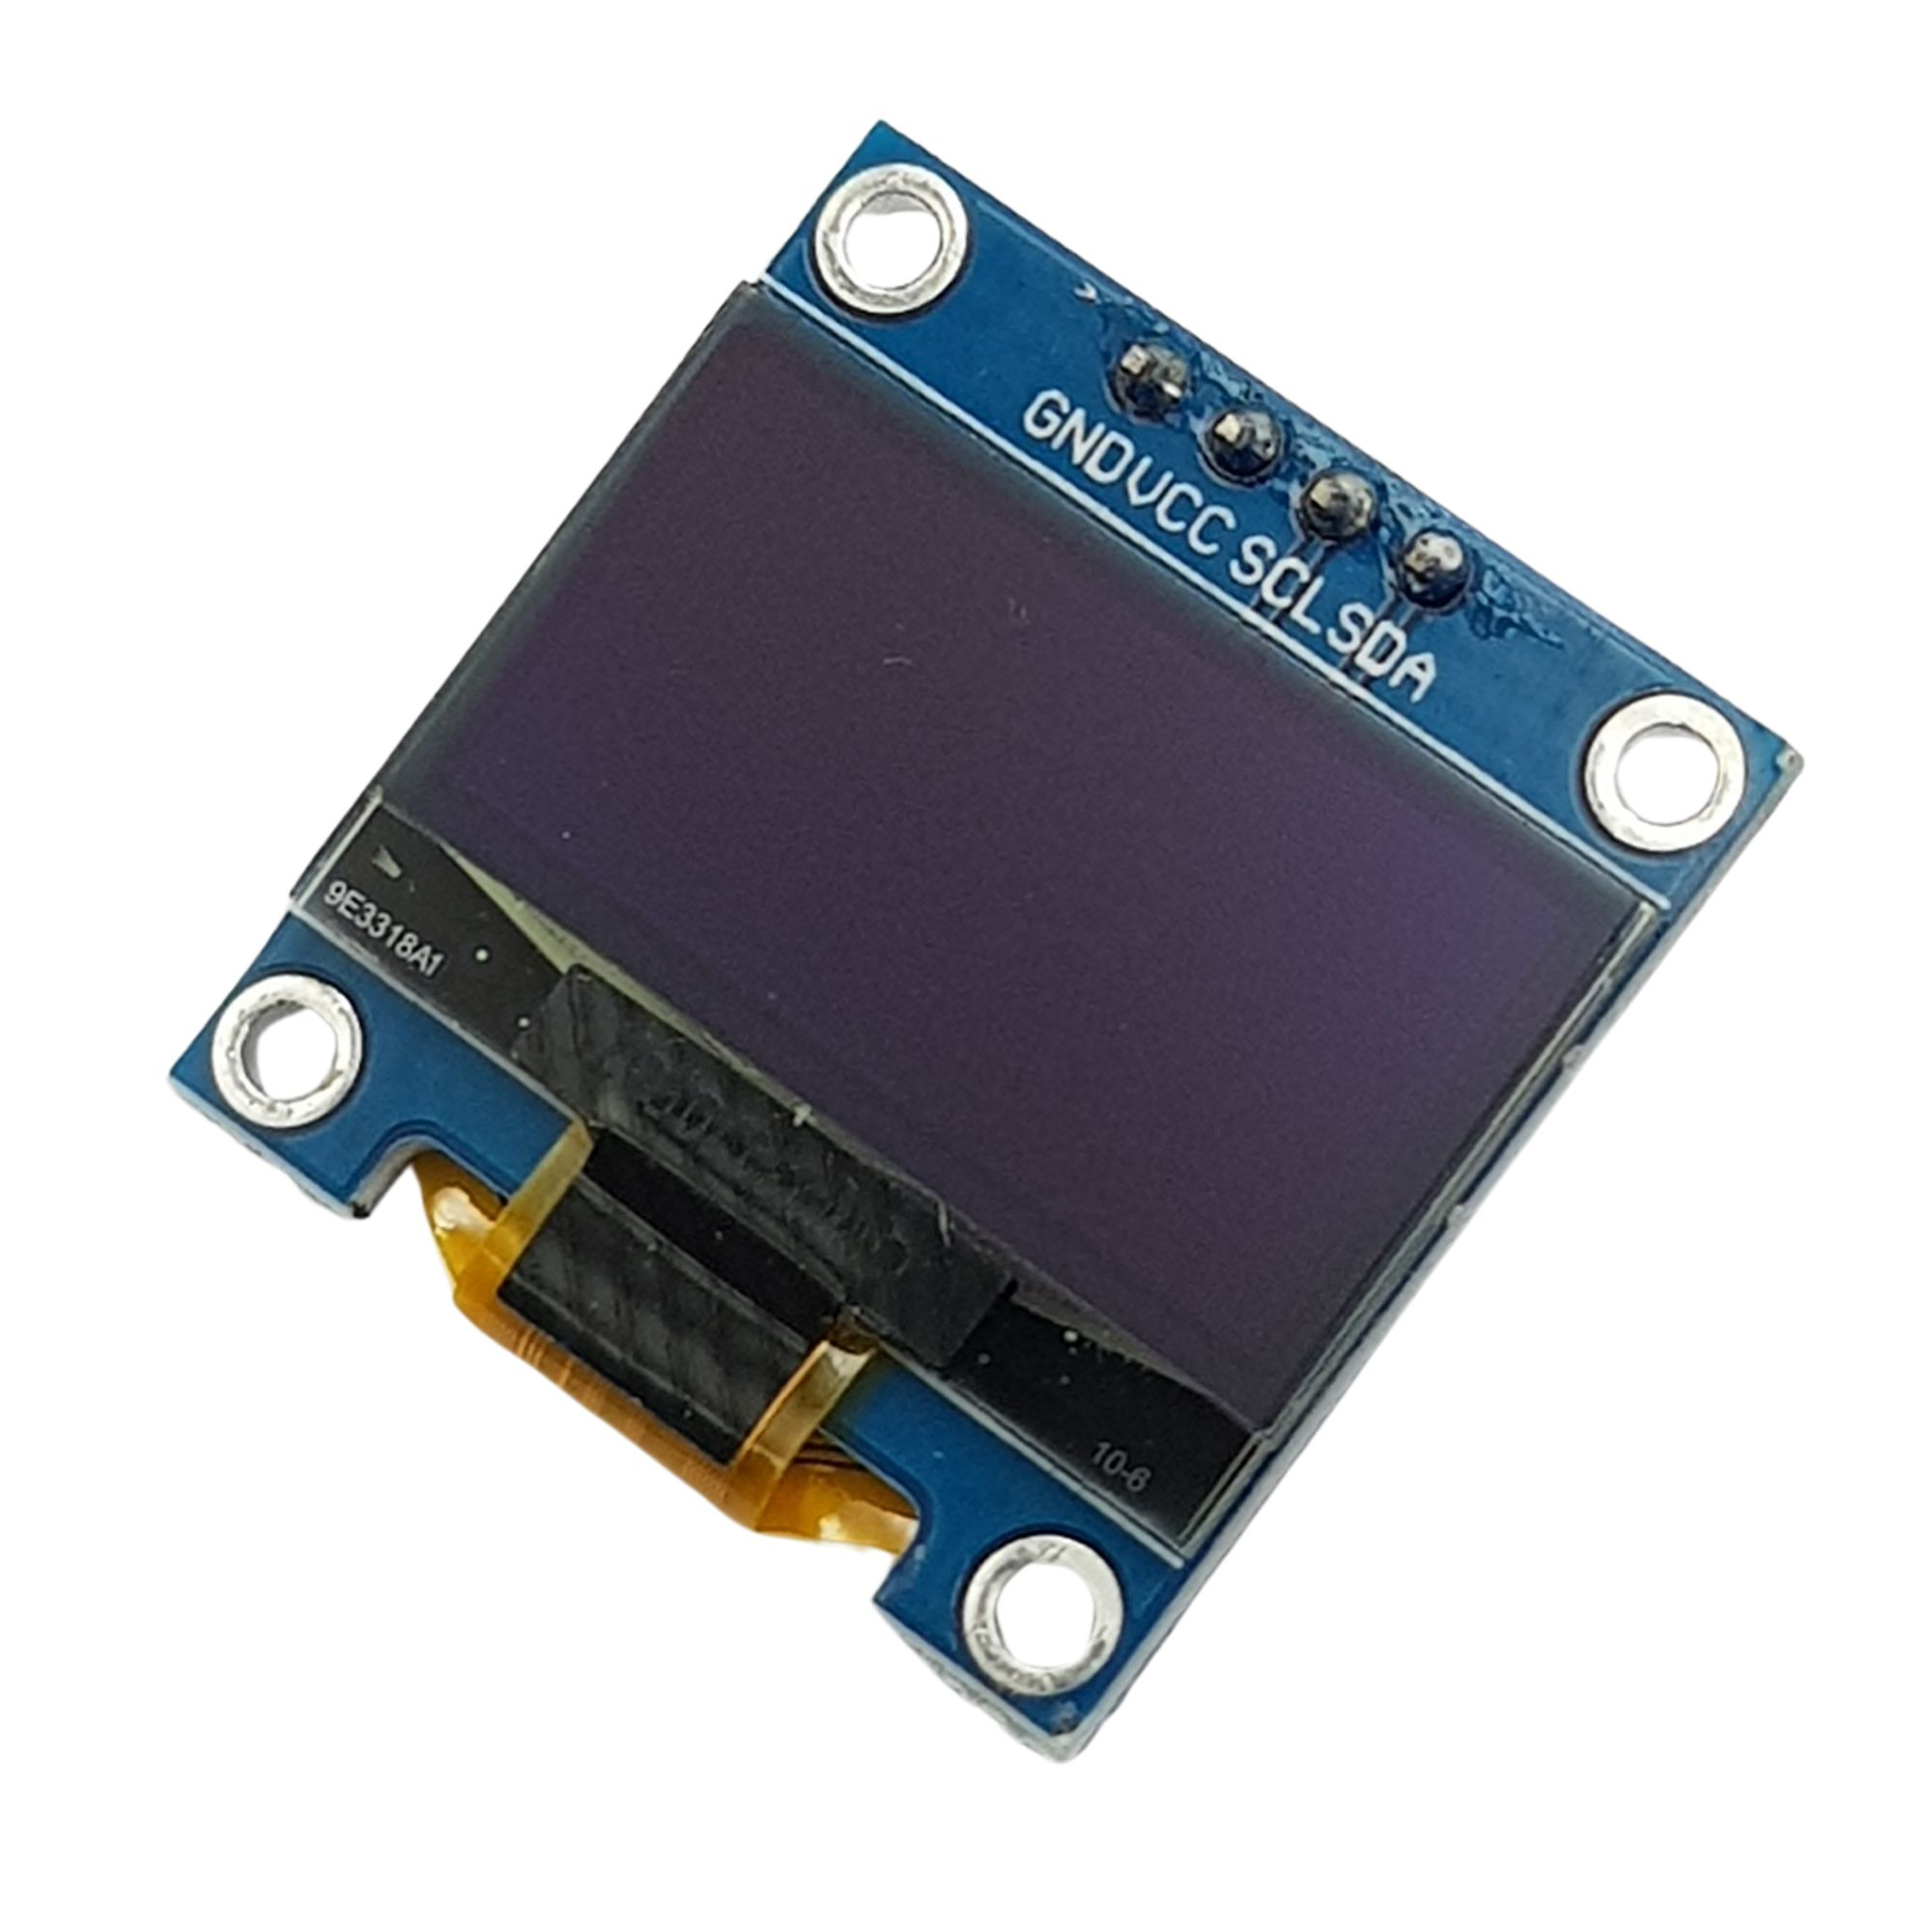
\includegraphics[width=0.5\linewidth]{oled096.jpg}
    \caption{Màn hình OLED 0.96 Inch 128x64}
    \label{fig:oled096}
\end{figure}

\subsubsection{Nguyên lý công nghệ hiển thị OLED}

OLED (Organic Light Emitting Diode) là công nghệ đi-ốt phát quang hữu cơ. Khác với màn hình LCD (Liquid Crystal Display) truyền thống sử dụng một tấm đèn nền (Backlight) chiếu sáng liên tục xuyên qua các tinh thể lỏng, màn hình OLED hoạt động dựa trên hiện tượng phát quang điện từ (Electroluminescence) của vật liệu hữu cơ. Khi có một điện áp được đặt giữa cực Anode và Cathode, các lỗ trống và electron sẽ di chuyển và tái hợp tại lớp phát sáng hữu cơ, giải phóng năng lượng dưới dạng photon ánh sáng.

Nhờ khả năng "tự phát sáng" tại từng điểm ảnh (pixel), màn hình OLED có thể tắt hoàn toàn các pixel tại vùng hiển thị màu đen. Điều này tạo ra độ tương phản gần như vô hạn, không có hiện tượng hở sáng (light bleeding) và mức tiêu thụ năng lượng cực thấp (chỉ khoảng 20mA - 30mA khi hiển thị văn bản).

\subsubsection{Giao thức I2C (Inter-Integrated Circuit)}

Để điều khiển 8192 điểm ảnh (128x64 pixel), module sử dụng IC điều khiển SSD1306 tích hợp bộ nhớ GDDRAM (Graphic Display Data RAM) tĩnh dung lượng 1KB. Thay vì sử dụng chuẩn SPI song song tốn nhiều chân GPIO, module OLED này giao tiếp với ESP32 thông qua bus I2C đa chủ - đa tớ (Multi-master, Multi-slave).

I2C hoạt động thông qua hai đường tín hiệu truyền dẫn đồng bộ:

\begin{itemize}
    \item SDA (Serial Data Line): Đường truyền dữ liệu hai chiều dạng nối tiếp.
    \item SCL (Serial Clock Line): Đường xung nhịp đồng bộ, được tạo ra bởi thiết bị Chủ (ESP32).
\end{itemize}

Quá trình giao tiếp bắt đầu khi ESP32 kéo đường SDA xuống mức Thấp (LOW) trong khi SCL đang ở mức Cao (HIGH), tạo ra điều kiện Khởi động (Start Condition). Tiếp theo, ESP32 gửi đi byte Địa chỉ thiết bị (Device Address - của màn hình OLED thường là 0x3C). SSD1306 nhận dạng địa chỉ và trả về một bit xác nhận (ACK). Sau đó, ESP32 tiến hành truyền các luồng dữ liệu (Data frames) chứa mã lệnh cấu hình (Command) hoặc mã ma trận điểm ảnh (Data) vào vùng nhớ GDDRAM, quá trình kết thúc bằng điều kiện Dừng (Stop Condition). Tốc độ truyền tải I2C trong cấu hình mặc định đạt 100 kHz (Standard-mode) hoặc 400 kHz (Fast-mode), hoàn toàn đáp ứng được tốc độ làm tươi màn hình thời gian thực của đồ án.

\subsection{Còi báo hiệu chủ động (Active Buzzer) và Hiệu ứng Áp điện}

\newpage
\begin{figure}
    \centering
    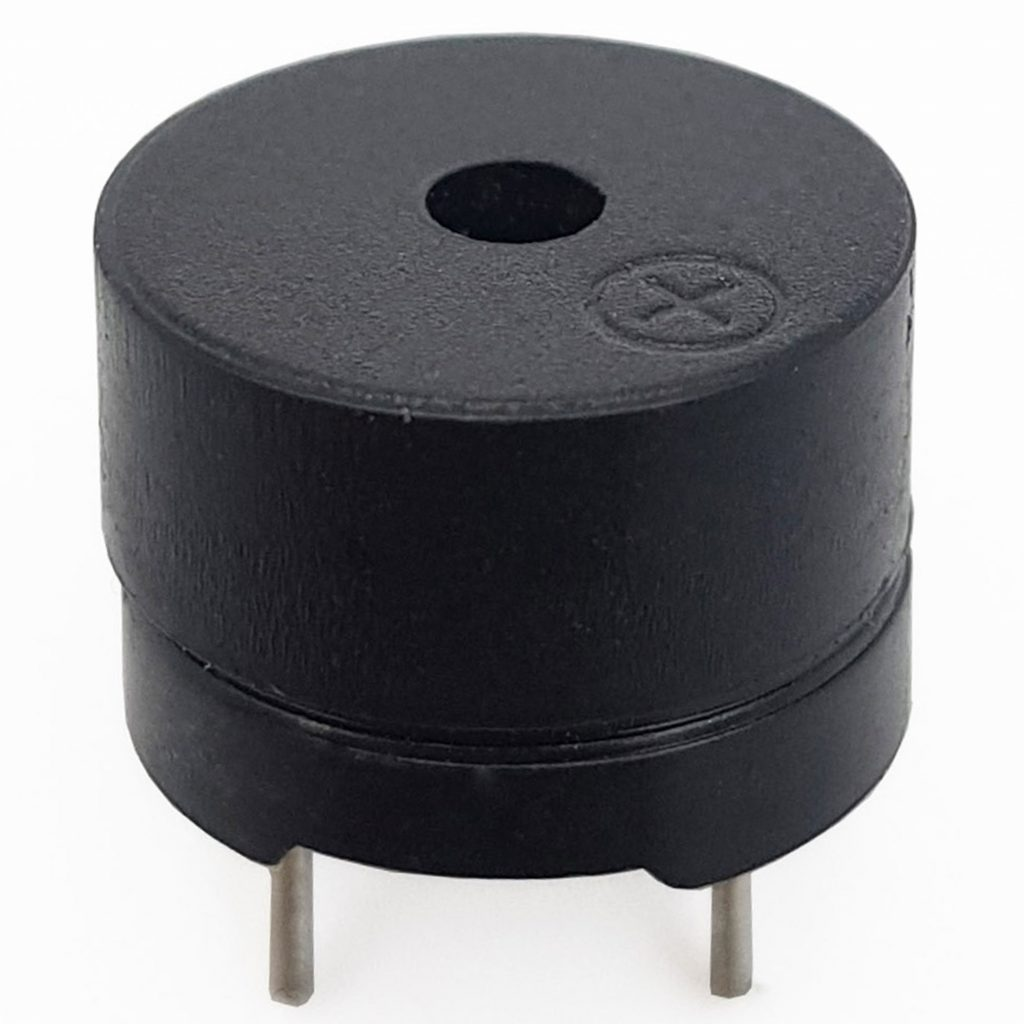
\includegraphics[width=0.5\textwidth]{buzzer.jpg}
    \caption{Buzzer Chirp}
    \label{fig:buzzer}
\end{figure}

\newpage
\subsubsection{Cấu trúc và Hiệu ứng Áp điện nghịch}

Buzzer trong đề tài sử dụng bộ chuyển đổi âm thanh dạng áp điện (Piezoelectric transducer). Thành phần cốt lõi của nó là một đĩa gốm áp điện (thường làm từ vật liệu Lead Zirconate Titanate - PZT) được dán chặt vào một tấm màng kim loại mỏng (màng rung).

Nguyên lý hoạt động dựa trên Hiệu ứng áp điện nghịch (Inverse Piezoelectric Effect): Khi đặt một điện trường (bằng cách cấp điện áp) xuyên qua màng gốm PZT, mạng tinh thể của vật liệu sẽ bị biến dạng cơ học (co lại hoặc giãn ra). Khi đặt một dòng điện xoay chiều (AC) vào đĩa gốm, sự biến dạng liên tục và có chu kỳ sẽ khiến tấm màng kim loại uốn cong qua lại, từ đó đẩy lớp không khí xung quanh, tạo ra sóng âm thanh truyền đến tai người.

\subsubsection{Kiến trúc Mạch dao động nội (Active Circuitry)}

Khác biệt hoàn toàn với Passive Buzzer (cần vi điều khiển cấp xung PWM xoay chiều để tạo âm thanh), Active Buzzer được coi là một "linh kiện thông minh" độc lập vì nó tích hợp sẵn một mạch dao động đa hài (Multivibrator Oscillator circuit) ngay trên bo mạch nền của vỏ còi.

Mạch dao động này thường bao gồm các transistor và tụ điện, thiết lập sẵn một dải tần số cộng hưởng cố định (ví dụ: 2500 Hz). Khi vi điều khiển ESP32 xuất một tín hiệu logic mức CAO (3.3V) từ chân GPIO vào chân điều khiển của Buzzer, tín hiệu điện một chiều (DC) này sẽ cung cấp năng lượng cho mạch đa hài. Mạch đa hài tự động băm dòng điện DC thành các xung vuông AC ở tần số 2500 Hz và cấp thẳng vào đĩa áp điện. Nhờ đặc tính này, hệ thống nhúng giảm tải được hoàn toàn việc phải sử dụng các bộ định thời (Timer) phức tạp để tạo xung âm thanh, thay vào đó chỉ cần điều khiển trạng thái BẬT/TẮT ở tầng ứng dụng.

\subsection{Công tắc hành trình (Micro Limit Switch) và Cơ chế Cơ điện}

\begin{figure}[H]
    \centering
    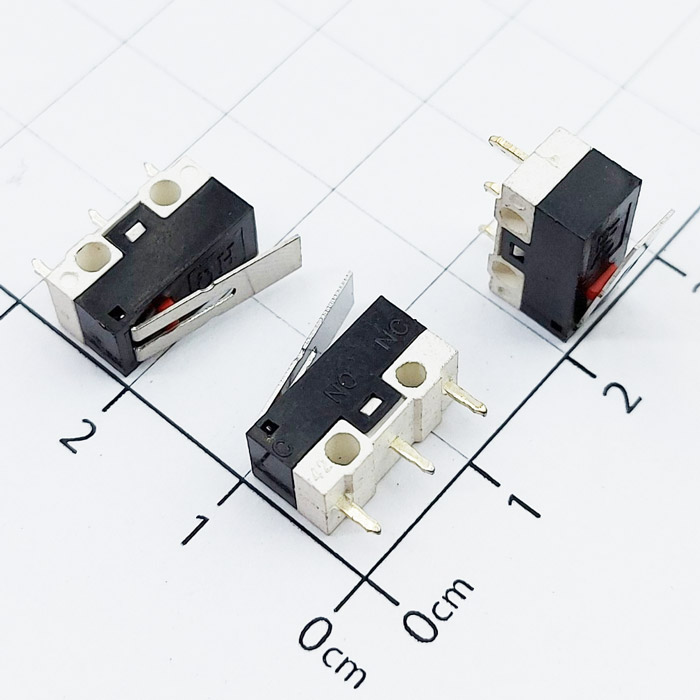
\includegraphics[width=0.5\textwidth]{switch.jpg}
    \caption{Công tắc hành trình}
    \label{fig:switch}
\end{figure}

\newpage
\subsubsection{Kiến trúc Đòn bẩy nảy}

Công tắc hành trình (Micro Switch) là một cảm biến tiếp xúc cơ học, đóng vai trò sống còn trong việc phát hiện trạng thái nắp hộp thuốc một cách chính xác tuyệt đối. Khác với các nút nhấn màng carbon tĩnh, Micro Switch hoạt động dựa trên cơ chế vật lý "Snap-action" (Cơ cấu đòn bẩy nảy hoặc Cơ cấu quá tâm - Over-center mechanism).

Bên trong công tắc là một hệ thống đòn bẩy kết hợp với một lò xo lá hợp kim có độ đàn hồi cao (Beryllium Copper). Các tiếp điểm được mạ Bạc (Ag) hoặc Vàng (Au) để giảm thiểu điện trở tiếp xúc. Cấu hình tiêu chuẩn là một rơ-le thu nhỏ dạng SPDT (Single Pole Double Throw) với 3 chân: COM (Chung), NO (Thường mở) và NC (Thường đóng).

\subsubsection{Động lực học chuyển mạch và Hiện tượng Dội phím (Bouncing)}

Khi nắp hộp đè lên cần gạt (Actuator), lực này truyền vào và làm uốn cong lò xo lá bên trong. Theo định luật Hooke, lò xo tích lũy thế năng đàn hồi. Ngay khi lực ép đẩy hệ thống vượt qua một "điểm tới hạn" (Operating Point), thế năng được giải phóng đột ngột. Lò xo bung ra, đá tiếp điểm động từ chân NC sang chân NO với vận tốc cực lớn (chỉ vài mili-giây).

Sự chênh lệch giữa Điểm tác động (Operating point) và Điểm nhả (Release point) tạo ra một khoảng trễ vật lý gọi là độ từ trễ cơ học (Mechanical Hysteresis). Đặc tính này vô cùng quan trọng: nó đảm bảo rằng dù nắp hộp có đóng mở một cách chậm chạp hay bị rung lắc nhẹ, tiếp điểm cũng không bao giờ nằm ở trạng thái lấp lửng, ngăn ngừa sự xuất hiện của hồ quang điện.
Tuy nhiên, sự va đập kim loại ở tốc độ cao chắc chắn sẽ gây ra hiện tượng Dội phím (Switch Bouncing) — tại khoảnh khắc đóng tiếp điểm, hai mặt kim loại sẽ nảy lên nảy xuống vài lần ở cấp độ vi mô, sinh ra một chuỗi các xung nhiễu điện tử trong khoảng 10-20ms đầu tiên. Nếu vi điều khiển đọc tín hiệu trong khoảng thời gian này, nó sẽ hiểu nhầm là nắp hộp bị mở/đóng hàng chục lần liên tiếp. Do đó, trong đồ án này, hiện tượng vật lý nêu trên đã được giải quyết triệt để bằng thuật toán Khử rung phần mềm (Software Debouncing) dựa trên bộ đếm thời gian \texttt{millis()} của ESP32, đảm bảo hệ thống chỉ ghi nhận một thao tác duy nhất sau khi trạng thái cơ học đã ổn định hoàn toàn.

\subsection{Module Thời gian thực (RTC) DS3231 và Cơ chế lưu trữ Offline}

\begin{figure}[H]
    \centering
    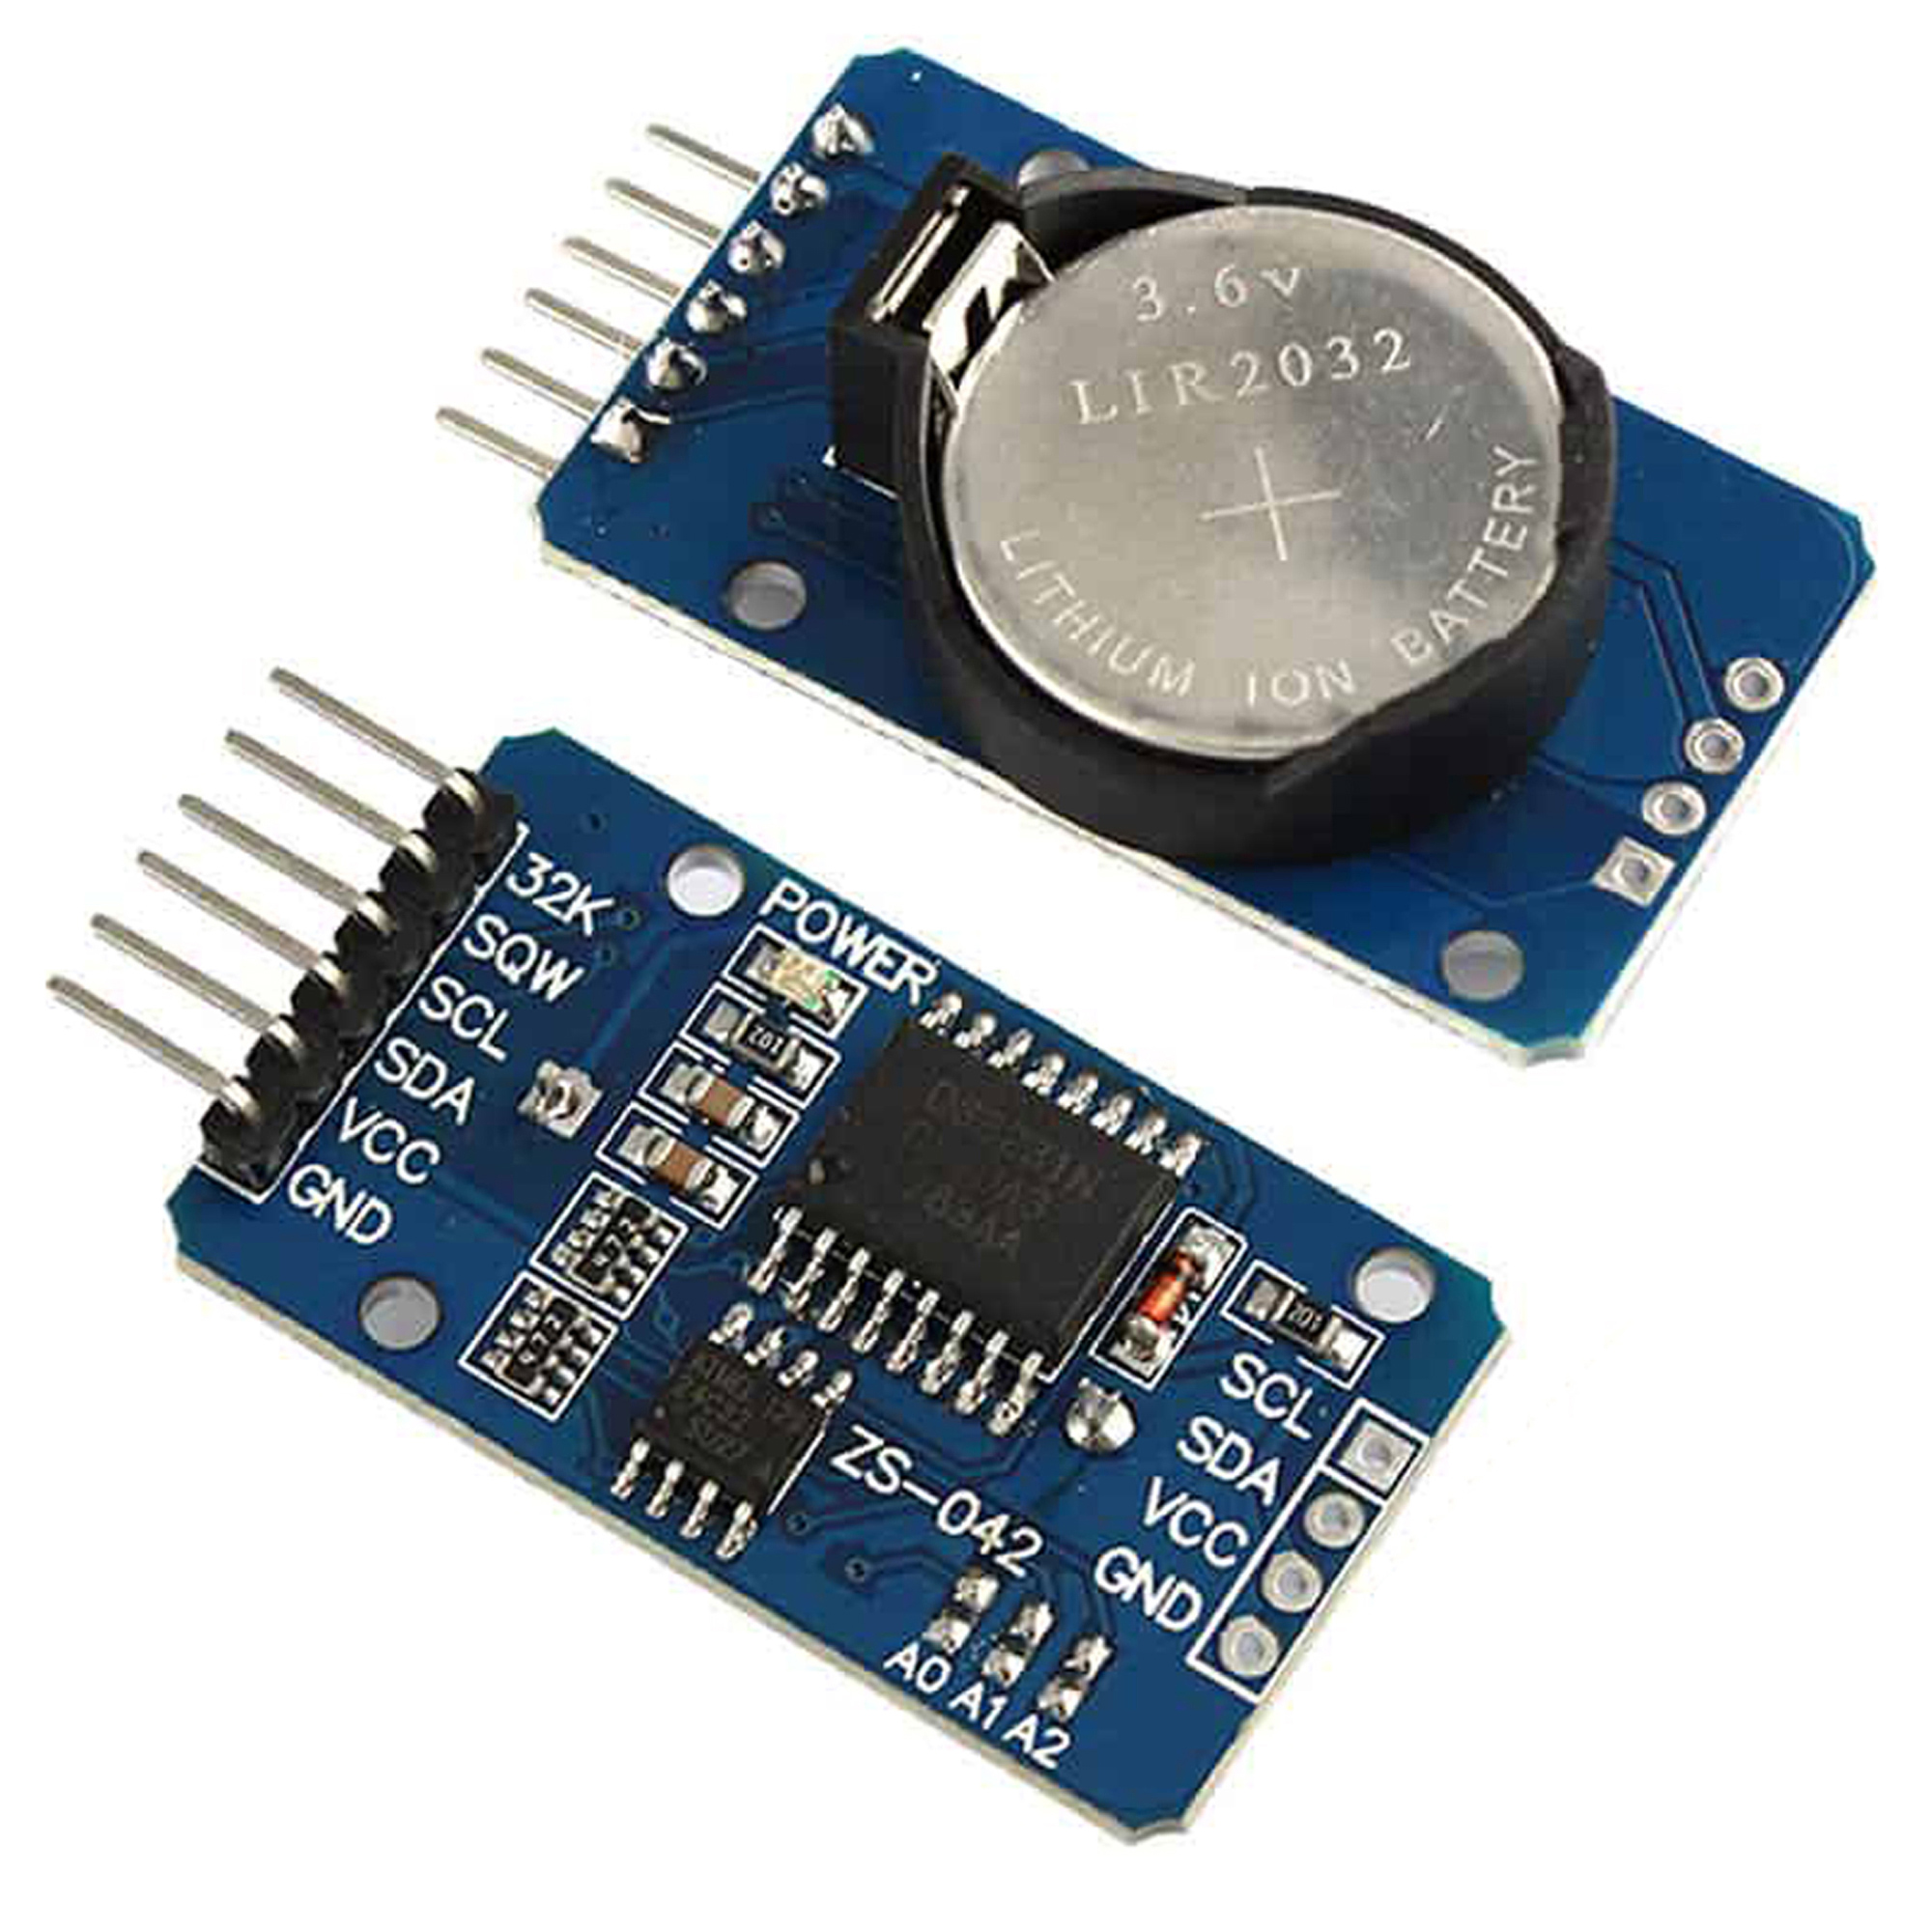
\includegraphics[width=0.5\textwidth]{ds3231.png}
    \caption{Module thời gian thực DS3231 tích hợp IC nhớ}
    \label{fig:ds3231}
\end{figure}

\subsubsection{Cấu trúc phần cứng và Bộ dao động bù nhiệt}

DS3231 là một vi mạch đồng hồ thời gian thực (Real-Time Clock) giao tiếp qua chuẩn I2C, được tích hợp sẵn bộ dao động thạch anh bù nhiệt (Temperature-Compensated Crystal Oscillator - TCXO) và một tinh thể thạch anh bên trong vỏ chip. Sự khác biệt lớn nhất của DS3231 so với các dòng RTC cơ bản là khả năng duy trì độ chính xác cực cao trong môi trường nhiệt độ biến đổi.

Ở các bộ dao động thông thường, tần số của thạch anh ($32.768\text{ kHz}$) sẽ bị sai lệch khi nhiệt độ môi trường thay đổi, dẫn đến hiện tượng trôi thời gian (time drift). Để khắc phục, DS3231 tích hợp một cảm biến nhiệt độ bên trong để liên tục đo đạc nhiệt độ của tinh thể thạch anh. Dựa vào giá trị này, vi mạch sẽ tự động điều chỉnh mảng tụ điện (capacitance array) bên trong để bù trừ lại sự sai lệch tần số. Nhờ vậy, sai số của DS3231 chỉ ở mức $\pm 2\text{ ppm}$ (tương đương sai lệch khoảng 1 phút mỗi năm).

Bên cạnh đó, DS3231 có thiết kế đường nguồn dự phòng (pin $V_{BAT}$). Khi nguồn cấp chính ($V_{CC}$) bị ngắt, mạch so sánh nội bộ sẽ tự động chuyển mạch sang nguồn pin dự phòng (Pin CMOS CR2032 3V) để duy trì hoạt động của bộ đếm thời gian mà không làm gián đoạn hệ thống.

\subsubsection{Tổ chức bộ nhớ và Định dạng dữ liệu BCD}

Dữ liệu thời gian bên trong DS3231 được lưu trữ tại các thanh ghi riêng biệt bao gồm: Giây, Phút, Giờ, Thứ, Ngày, Tháng và Năm. Mạch tự động tính toán số ngày trong các tháng có ít hơn 31 ngày và hỗ trợ tự động bù trừ năm nhuận (áp dụng đến năm 2100).

Dữ liệu trong các thanh ghi này được định dạng theo chuẩn BCD. Đây là hệ thống mã hóa số thập phân trong đó mỗi chữ số thập phân được biểu diễn bằng một chuỗi nhị phân 4 bit. Việc sử dụng BCD giúp vi điều khiển trung tâm dễ dàng trích xuất trực tiếp các giá trị hàng chục và hàng đơn vị của thời gian để hiển thị lên màn hình (như OLED) mà không cần thực hiện các phép chia nguyên hay lấy dư phức tạp, giúp tối ưu hóa chu kỳ lệnh của CPU.

\subsubsection{Hệ thống Báo thức kép và Ngắt phần cứng}

DS3231 được trang bị hai thanh ghi báo thức độc lập (Alarm 1 và Alarm 2). Hệ thống báo thức này cho phép lập trình viên thiết lập các mốc thời gian kích hoạt cụ thể (khớp theo giây, phút, giờ hoặc ngày).

Khi giá trị thời gian thực tế đếm đến mốc thời gian đã cài đặt trong thanh ghi Alarm, vi mạch sẽ tự động bật một cờ báo ngắt. Nếu được cấu hình, tín hiệu ngắt này sẽ được xuất ra chân SQW/INT (mức thấp tích cực). Trong các thiết kế hệ thống nhúng tiết kiệm năng lượng, đặc tính này đóng vai trò then chốt: Vi điều khiển chính có thể chuyển vào trạng thái ngủ sâu (Deep-sleep) để bảo toàn năng lượng, và chỉ bị "đánh thức" bởi tín hiệu ngắt phần cứng từ chân INT của DS3231 khi đến chính xác thời điểm cần thực thi nhiệm vụ.

\subsection{Module Quản lý Năng lượng và Tăng áp J5019}

\begin{figure}[H]
    \centering
    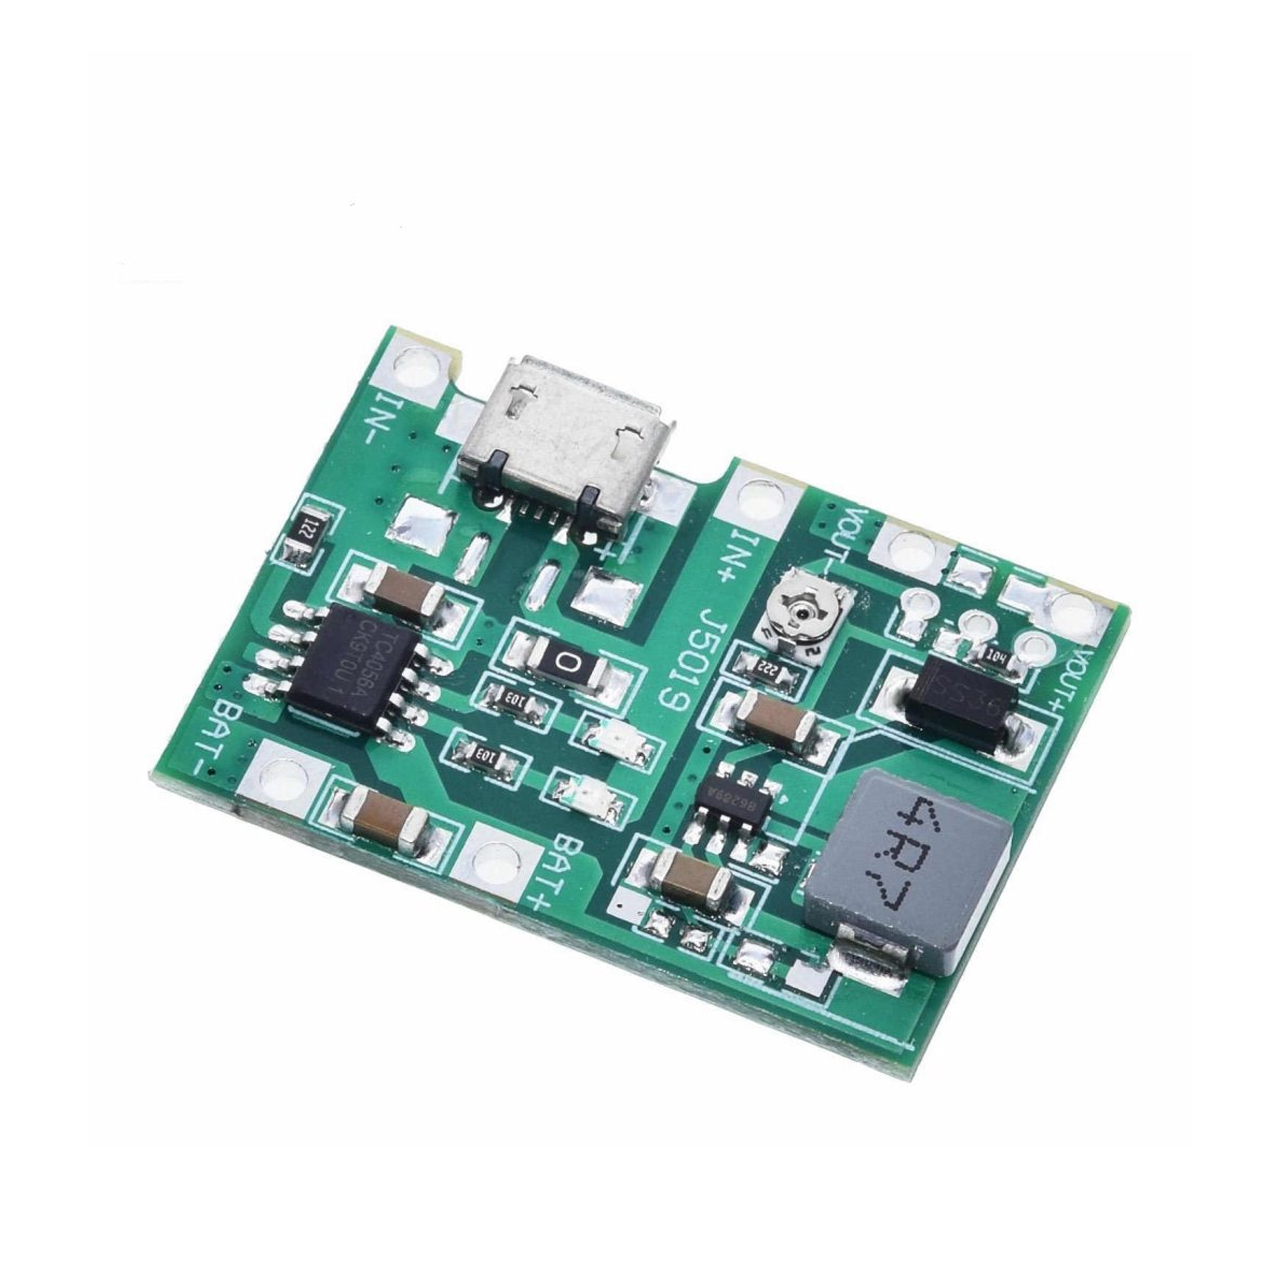
\includegraphics[width=0.5\linewidth]{j5019.png}
    \caption{Mạch sạc tích hợp Boost DC-DC J5019}
    \label{fig:j5019}
\end{figure}

\subsubsection{Cấu trúc phần cứng và Tích hợp hệ thống}
Module J5019 là một giải pháp thiết kế phần cứng kết hợp giữa mạch sạc pin Lithium-ion 1 cell (3.7V) và mạch chuyển đổi điện áp nâng áp (DC-DC Boost Converter). Trong các hệ thống IoT nhúng yêu cầu tính liên tục như dự án hộp thuốc thông minh, module này đóng vai trò trọng yếu trong việc đảm bảo vi điều khiển trung tâm ESP32 và các cảm biến ngoại vi luôn được cấp một mức điện áp hoạt động ổn định (tùy chỉnh ở mức 5V hoặc 9V), ngay cả khi điện áp định mức của cell pin suy giảm dần trong chu kỳ xả. Nền tảng board mạch hỗ trợ cấp nguồn đầu vào đa dạng thông qua cổng Micro USB/Type-C hoặc các vị trí hàn trực tiếp, đồng thời cho phép tinh chỉnh điện áp đầu ra linh hoạt thông qua một biến trở tích hợp.

\subsubsection{Nguyên lý Sạc tuyến tính (Linear Charging) và Cơ chế CC/CV}
Khối sạc của module vận hành dựa trên vi mạch chuyên dụng TP4056. Quá trình nạp năng lượng cho pin Lithium được giám sát và điều khiển nghiêm ngặt thông qua thuật toán Dòng không đổi / Áp không đổi (CC/CV - Constant Current / Constant Voltage) nhằm tối ưu hóa tuổi thọ và đảm bảo an toàn hóa học bên trong cell pin:
\begin{itemize}
    \item \textbf{Sạc nhỏ giọt (Trickle Charge):} Khi điện áp pin sụt xuống dưới ngưỡng an toàn (thường là 2.9V), vi mạch chỉ cấp một dòng sạc rất nhỏ (khoảng 10\% dòng định mức) để phục hồi áp từ từ, ngăn ngừa hiện tượng sốc nhiệt và phá vỡ cấu trúc hóa học của pin.
    \item \textbf{Dòng không đổi (Constant Current):} Khi điện áp pin vượt ngưỡng 2.9V, mạch tự động chuyển sang trạng thái bơm dòng tối đa (có thể lên đến 1A tùy thuộc vào điện trở lập trình $R_{PROG}$) để nạp nhanh dung lượng.
    \item \textbf{Áp không đổi (Constant Voltage):} Khi điện áp trên hai cực của pin tiệm cận mức sạc đầy 4.2V, mạch sẽ duy trì ổn định mức áp này trong khi dòng sạc bắt đầu suy giảm theo hàm đồ thị mũ. Quá trình sạc sẽ tự động ngắt hoàn toàn (Termination) khi dòng điện giảm xuống dưới ngưỡng cắt.
\end{itemize}

\subsubsection{Nguyên lý Mạch Tăng áp (DC-DC Boost) và Động lực học Chuyển mạch}
Khối nâng áp ứng dụng kiến trúc chuyển mạch tần số cao, sử dụng IC MT3608 hoạt động ở xung nhịp xấp xỉ 1.2MHz. Việc triển khai tần số chuyển mạch lớn cho phép tối thiểu hóa kích thước vật lý của cuộn cảm (Inductor) và tụ lọc (Capacitor) trên không gian board mạch. Quá trình biến đổi mức điện áp tuân theo chu kỳ của hai pha cơ bản:
\begin{itemize}
    \item \textbf{Pha tích lũy (Switch ON):} Khi MOSFET nội bộ được kích dẫn, dòng điện từ nguồn pin đi qua cuộn cảm xuống mass, khiến cuộn cảm tích lũy năng lượng dưới dạng từ trường.
    \item \textbf{Pha giải phóng (Switch OFF):} Khi MOSFET ngắt, từ trường trong cuộn cảm sụp đổ và sinh ra sức điện động cảm ứng. Điện áp này cộng gộp nối tiếp với điện áp nguồn pin, vượt qua điện áp phân cực của Diode Schottky và xả năng lượng định tuyến vào tụ điện ngõ ra.
\end{itemize}

Trị số điện áp đầu ra được kiểm soát bởi mạng điện trở phân áp (Feedback resistor network) thông qua phương trình:
\begin{equation}
    V_{out} = V_{ref} \times \left(1 + \frac{R_1}{R_2}\right)
\end{equation}
Trong đó, $V_{ref}$ là điện áp tham chiếu nội bộ (thường là 0.6V), $R_1$ và $R_2$ là các trị số điện trở cấu thành trên nhánh phản hồi. Khi triển khai mạch in (PCB) trên phần mềm Altium Designer, quá trình đi dây khu vực này cần tách biệt vùng nhiễu chuyển mạch tần số cao ra khỏi các đường tín hiệu I2C hoặc Logic nhạy cảm để tránh hiện tượng sai số dữ liệu.

\newpage
\begin{center}
    \section{THIẾT KẾ VÀ THỰC HIỆN PHẦN CỨNG}
\end{center}
%Nội dung chương 3
\subsection{Sơ đồ khối tổng quát của hệ thống}
Hệ thống được thiết kế dựa trên sự tương tác giữa 4 khối chức năng chính: Khối nguồn, Khối xử lý trung tâm, Khối ngõ vào và Khối ngõ ra.

\begin{itemize}
    \item \textbf{Khối Nguồn:} Sử dụng pin Lithium-Ion 3.7V kết hợp mạch quản lý năng lượng J5019. Dòng điện từ pin được tăng áp lên mức 5V ổn định để cung cấp năng lượng cho toàn hệ thống.
    \item \textbf{Khối Xử lý trung tâm:} Vi điều khiển ESP32 chịu trách nhiệm thu thập tín hiệu cảm biến, điều khiển ngoại vi hiển thị, xử lý thuật toán thời gian và giao tiếp vô tuyến với hệ thống máy chủ.
    \item \textbf{Khối Ngõ vào:} Bao gồm đồng hồ thời gian thực DS3231 cung cấp mốc thời gian chuẩn xác và công tắc hành trình để nhận diện thao tác đóng hoặc mở nắp hộp. Mạch còn được tích hợp thêm khối chia áp để đo lường dung lượng pin hiện tại.
    \item \textbf{Khối Ngõ ra:} Màn hình OLED hiển thị thông tin trực quan và còi báo động để phát ra âm thanh cảnh báo khi đến cữ thuốc.
\end{itemize}

\begin{figure}[H]
    \centering
    \begin{tikzpicture}[
        scale=0.85, transform shape,
        box/.style = {rectangle, draw=black, thick, fill=blue!10, text width=3.2cm, align=center, minimum height=2.2cm, rounded corners},
        power/.style = {rectangle, draw=black, thick, fill=red!10, text width=3.2cm, align=center, minimum height=1.2cm, rounded corners},
        input/.style = {rectangle, draw=black, thick, fill=green!10, text width=2.8cm, align=center, minimum height=1.2cm, rounded corners},
        output/.style = {rectangle, draw=black, thick, fill=yellow!10, text width=2.8cm, align=center, minimum height=1.2cm, rounded corners},
        arrow/.style = {thick, ->, >=stealth},
        bidi/.style = {thick, <->, >=stealth}
    ]

    % --- KHAI BÁO CÁC KHỐI ---
    
    \node[box] (esp) {\textbf{Khối Xử lý trung tâm} \\ ESP32 NodeMCU};

    \node[power, above=1.2cm of esp] (power) {\textbf{Khối Nguồn} \\ Pin Li-Po 3.7V \\ + Boost J5019};

    % Khối Ngõ vào (Tách xa nhau ra để không đè, tạo không gian cho chữ L)
    \node[input, left=2.5cm of esp, yshift=2.7cm] (rtc) {\textbf{Thời gian thực} \\ Module RTC DS3231};
    \node[input, left=2.5cm of esp, yshift=-2.7cm] (switch) {\textbf{Cảm biến} \\ Công tắc hành trình};

    % Khối Ngõ ra (Tương tự, tách đều lên xuống)
    \node[output, right=2.5cm of esp, yshift=2.7cm] (oled) {\textbf{Khối Hiển thị} \\ Màn hình OLED 0.96 inch};
    \node[output, right=2.5cm of esp, yshift=-2.7cm] (buzzer) {\textbf{Khối Cảnh báo} \\ Còi Buzzer};

    % --- VẼ MŨI TÊN KẾT NỐI (ĐƯỜNG CHỮ L) ---
    
    % Nguồn -> ESP32 (Đường thẳng từ trên xuống)
    \draw[arrow] (power) -- node[anchor=west, font=\small] {5V DC} (esp);
    
    % RTC <-> ESP32 (Chữ L: Từ DƯỚI đáy RTC đi xuống rồi rẽ phải vào mép trái ESP32)
    \draw[bidi] (rtc.south) |- node[above, font=\small, pos=0.75] {I2C} ([yshift=0.6cm]esp.west);
    
    % Switch -> ESP32 (Chữ L: Từ ĐỈNH Switch đi lên rồi rẽ phải vào mép trái ESP32)
    \draw[arrow] (switch.north) |- node[above, font=\small, pos=0.75] {Digital} ([yshift=-0.6cm]esp.west);
    
    % ESP32 -> OLED (Chữ L: Từ mép phải ESP32 đi ngang ra rồi rẽ CẮM LÊN đáy OLED)
    \draw[arrow] ([yshift=0.6cm]esp.east) -| node[above, font=\small, pos=0.25] {I2C} (oled.south);
    
    % ESP32 -> Buzzer (Chữ L: Từ mép phải ESP32 đi ngang ra rồi CẮM XUỐNG đỉnh Buzzer)
    \draw[arrow] ([yshift=-0.6cm]esp.east) -| node[above, font=\small, pos=0.25] {Digital} (buzzer.north);

    \end{tikzpicture}
    \caption{Sơ đồ khối tổng quát hệ thống Hộp Thuốc IoT}
    \label{fig:so_do_khoi_tikz}
\end{figure}

\subsection{Tính toán và lựa chọn linh kiện}
Việc lựa chọn và bổ sung linh kiện được cân nhắc kỹ lưỡng nhằm khắc phục các vấn đề vật lý phát sinh và đảm bảo tính ổn định của thiết bị:
\subsubsection{Vi điều khiển trung tâm ESP32}
Đối với một thiết bị y tế cá nhân phân tán chạy bằng năng lượng pin, vi điều khiển trung tâm đòi hỏi phải cân bằng giữa năng lực tính toán hiệu năng cao và khả năng tiết kiệm năng lượng tối ưu. Bo mạch phát triển ESP32 NodeMCU Devkit V1 được lựa chọn dựa trên các luận cứ kỹ thuật sau:
\begin{itemize}
    \item \textbf{Kiến trúc lõi kép xử lý bất đồng bộ:} Vi xử lý kiến trúc lõi kép 32-bit cho phép phân tách luồng tác vụ chạy ngầm của ngăn xếp giao thức mạng vô tuyến và luồng thuật toán ứng dụng của người dùng trên hai lõi độc lập, giải quyết triệt để hiện tượng nghẽn lệnh hoặc treo hệ thống khi chờ kết nối máy chủ.
    \item \textbf{Cơ chế quản lý năng lượng linh hoạt:} ESP32 hỗ trợ cấu hình hạ xung nhịp hoạt động của CPU xuống mức 80MHz và cung cấp chế độ ngủ sâu. Trong trạng thái ngủ, toàn bộ lõi xử lý và module vô tuyến được ngắt điện hoàn toàn, dòng tiêu thụ giảm xuống mức vi-ampe, đóng vai trò kéo dài chu kỳ sống của pin.
    \item \textbf{Tài nguyên bộ nhớ tích hợp lớn:} Dung lượng bộ nhớ SRAM lớn cho phép xử lý và phân tích các chuỗi dữ liệu định dạng JSON phức tạp từ API đám mây trả về. Đồng thời, bộ nhớ Flash cho phép lưu trữ hệ thống tệp tin tĩnh và hàng đợi dữ liệu lịch sử khi thiết bị rớt mạng.
\end{itemize}

\subsubsection{Hệ thống nguồn và khối đo lường dung lượng pin}
Hệ thống nguồn được thiết kế hướng tới tính bền bỉ, an toàn hóa học và tối ưu không gian cơ khí của thiết bị:
\begin{itemize}
    \item \textbf{Module quản lý sạc và tăng áp J5019:} Linh kiện tích hợp sẵn vi mạch sạc tuyến tính chuyên dụng TP4056 và vi mạch biến đổi nâng áp một chiều chuyển mạch tần số cao MT3608 hoạt động ở xung nhịp 1.2MHz. Sự tích hợp này giúp loại bỏ hoàn toàn việc sử dụng hai module độc lập, tiết kiệm diện tích bo mạch in và giảm thiểu điện cảm ký sinh trên đường dây dẫn nguồn. Khối sạc vận hành theo cơ chế dòng không đổi và áp không đổi, đảm bảo an toàn tuyệt đối cho pin. Khối nâng áp cho phép điều chỉnh ngõ ra ổn định ở mức 5V phục vụ cho đường nguồn chính của hệ thống.
    \item \textbf{Pin nguồn Li-Ion hiệu năng cao:} Thay vì sử dụng các dòng pin Lithium Polymer giá rẻ có độ tin cậy thấp và độ suy hao dung lượng nhanh trên thị trường, đề tài ứng dụng giải pháp tái chế cell pin Lithium-Ion từ các dòng điện thoại thông minh chính hãng đã qua sử dụng. Các cell pin này sở hữu dung lượng thực tế đạt xấp xỉ 2000mAh, tích hợp sẵn mạch bảo vệ chạm chập nguyên bản của nhà sản xuất, đồng thời cung cấp dòng xả đỉnh cực kỳ ổn định. Giải pháp này vừa tối ưu chi phí thi công mạch, vừa đảm bảo độ an toàn chống phồng pin, cháy nổ vượt trội trong quá trình hoạt động dài hạn.
    \item \textbf{Khối bảo vệ nguồn khẩn cấp:} Khi module vô tuyến của ESP32 thực hiện kết nối mạng hoặc giải mã các giao thức bảo mật đám mây, dòng tiêu thụ biên của linh kiện có thể đột ngột vọt lên mức 350mA - 400mA trong khoảng thời gian mili-giây. Để triệt tiêu hiện tượng sụt áp cục bộ trên đường nguồn gây kích hoạt bộ giám sát điện áp thấp nội bộ làm vi điều khiển tự khởi động lại liên tục, một tụ hóa chất lượng cao có trị số 100uF được bổ sung kẹp song song tại ngõ vào nguồn 5V, đóng vai trò như một kho lưu trữ bù dòng tức thời.
    \item \textbf{Cầu phân áp giám sát năng lượng:} Để hệ thống nhận biết mức dung lượng pin hiện tại nhằm đưa ra cảnh báo sạc, điện áp trực tiếp từ cell pin được đưa qua một cầu chia áp gồm hai điện trở có trị số lớn 100k mắc nối tiếp xuống mass. Điện áp pin cực đại ở mức sạc đầy (4.2V) qua cầu phân áp sẽ giảm tuyến tính xuống mức 2.1V, hoàn toàn tương thích với ngưỡng đọc an toàn của bộ chuyển đổi tương tự - số trên chân D34 của ESP32. Việc lựa chọn giá trị điện trở lên đến 100k giúp giới hạn dòng rò tiêu hao qua nhánh đo lường ở mức siêu nhỏ, không làm ảnh hưởng đến tổng dung lượng chung của pin:
    \begin{equation}
        I_{leak} = \frac{V_{bat}}{R_{bat1} + R_{bat2}} = \frac{4.2V}{100k\Omega + 100k\Omega} = 21\mu A
    \end{equation}
\end{itemize}

\subsubsection{Tính toán thời gian vận hành lý thuyết}
Dòng điện tiêu thụ tổng thể của hệ thống được tính toán dựa trên chu kỳ hoạt động đặc thù của một thiết bị nhắc nhở y tế cá nhân:
\begin{itemize}
    \item Dòng điện trung bình ở chế độ hoạt động (Active Mode): $\approx 120$ mA.
    \item Dòng điện trung bình ở chế độ ngủ (Deep-sleep Mode): $\approx 5$ mA (bao gồm dòng tĩnh của module thời gian thực và dòng rò chuyển mạch của cuộn cảm trên mạch tăng áp).
    \item Kịch bản vận hành giả định: Thiết bị thức tổng cộng 30 phút (0.5 giờ) mỗi ngày để thực hiện hiển thị, phát cảnh báo chuông và đồng bộ dữ liệu mạng; thời gian còn lại 23.5 giờ thiết bị nằm ở trạng thái ngủ tiết kiệm năng lượng.
\end{itemize}
Điện năng tiêu thụ định mức trong một ngày của hệ thống được xác định qua phương trình:
\begin{equation}
    C_{day} = (120\text{ mA} \times 0.5\text{ h}) + (5\text{ mA} \times 23.5\text{ h}) = 60\text{ mAh} + 117.5\text{ mAh} = 177.5\text{ mAh}
\end{equation}
Với cell pin Lithium-Ion dung lượng 2000mAh, thời gian hoạt động liên tục lý thuyết của hộp thuốc trước khi cần kết nối bộ sạc là:
\begin{equation}
    T_{operation} = \frac{2000\text{ mAh}}{177.5\text{ mAh/ngày}} \approx 11.27\text{ ngày}
\end{equation}
Kết quả tính toán chứng minh hệ thống hoàn toàn đáp ứng tiêu chuẩn của một thiết bị y tế di động tầm trung, giảm thiểu tần suất phải cắm sạc cho người dùng.

\subsubsection{Module thời gian thực DS3231}
Để đảm bảo tính năng báo thức hoạt động chính xác tuyệt đối kể cả khi mất kết nối mạng, đồng hồ thời gian thực độc lập DS3231 được trang bị với các đặc tính kỹ thuật vượt trội:
\begin{itemize}
    \item \textbf{Bộ dao động thạch anh bù nhiệt:} Tích hợp sẵn cảm biến nhiệt độ nội vi và mảng tụ điện linh hoạt bên trong vỏ chip. Cơ chế này liên tục đo đạc biên độ nhiệt môi trường để hiệu chỉnh tần số dao động của tinh thể thạch anh, khống chế sai số thời gian ở mức cực thấp, không bị hiện tượng lệch giờ do nhiệt độ phòng biến đổi.
    \item \textbf{Cơ chế duy trì nguồn độc lập:} Module được trang bị đường nguồn dự phòng thông qua rào cắm kết nối với pin cúc áo CR2032. Khi nguồn điện chính của hộp thuốc bị ngắt hoàn toàn, vi mạch tự động chuyển đổi sang nguồn pin dự phòng để nuôi bộ đếm thời gian nội bộ, đảm bảo tính toàn vẹn dữ liệu lịch trình.
\end{itemize}

\subsubsection{Cảm biến và ngoại vi hiển thị, cảnh báo}
\begin{itemize}
    \item \textbf{Công tắc hành trình cơ học:} Lựa chọn công tắc dạng đòn bẩy gạt nảy dựa trên cơ cấu quá tâm. Tiếp điểm cơ học SPDT giúp triệt tiêu hoàn toàn dòng điện nuôi ở trạng thái chờ so với cảm biến hồng ngoại. Linh kiện mang lại phản hồi đóng cắt chắc chắn khi đóng mở nắp hộp. Hiện tượng dội phím cơ học phát sinh trong khoảng 10-20ms đầu tiên của tiếp điểm được xử lý dứt điểm bằng bộ lọc phần mềm.
    \item \textbf{Màn hình hiển thị OLED 0.96 inch:} Sử dụng IC điều khiển SSD1306, giao tiếp qua bus số I2C. Công nghệ tự phát sáng tại từng điểm ảnh hữu cơ giúp loại bỏ đèn nền, mang lại độ tương phản cao, góc nhìn rộng phù hợp cho mắt người cao tuổi và mức tiêu thụ dòng cực thấp.
    \item \textbf{Còi cảnh báo chủ động:} Tích hợp sẵn mạch dao động đa hài bên trong vỏ còi. Vi điều khiển chỉ cần xuất mức logic cao từ chân GPIO để cấp nguồn, còi sẽ tự động băm dòng điện thành các xung vuông tần số 2500Hz ổn định, giảm tải hoàn toàn chu kỳ xung phần mềm cho CPU.
\end{itemize}

\subsection{Thiết kế sơ đồ nguyên lý (Schematic)}
Sơ đồ nguyên lý của hệ thống được xây dựng và chuẩn hóa trên công nghệ thiết kế của phần mềm Altium Designer. Toàn bộ cấu trúc mạch tuân thủ nghiêm ngặt nguyên lý mô-đun hóa: tất cả các module chức năng và đường kết nối ngoại vi đều giao tiếp thông qua hệ thống các rào cắm (Header) đực-cái tiêu chuẩn bước chân 2.54mm, hạn chế tối đa việc hàn nhiệt trực tiếp lên thân linh kiện nhạy cảm, giúp bo mạch có tính tùy biến cao và dễ dàng bảo trì.

\begin{figure}[H]
    \centering
    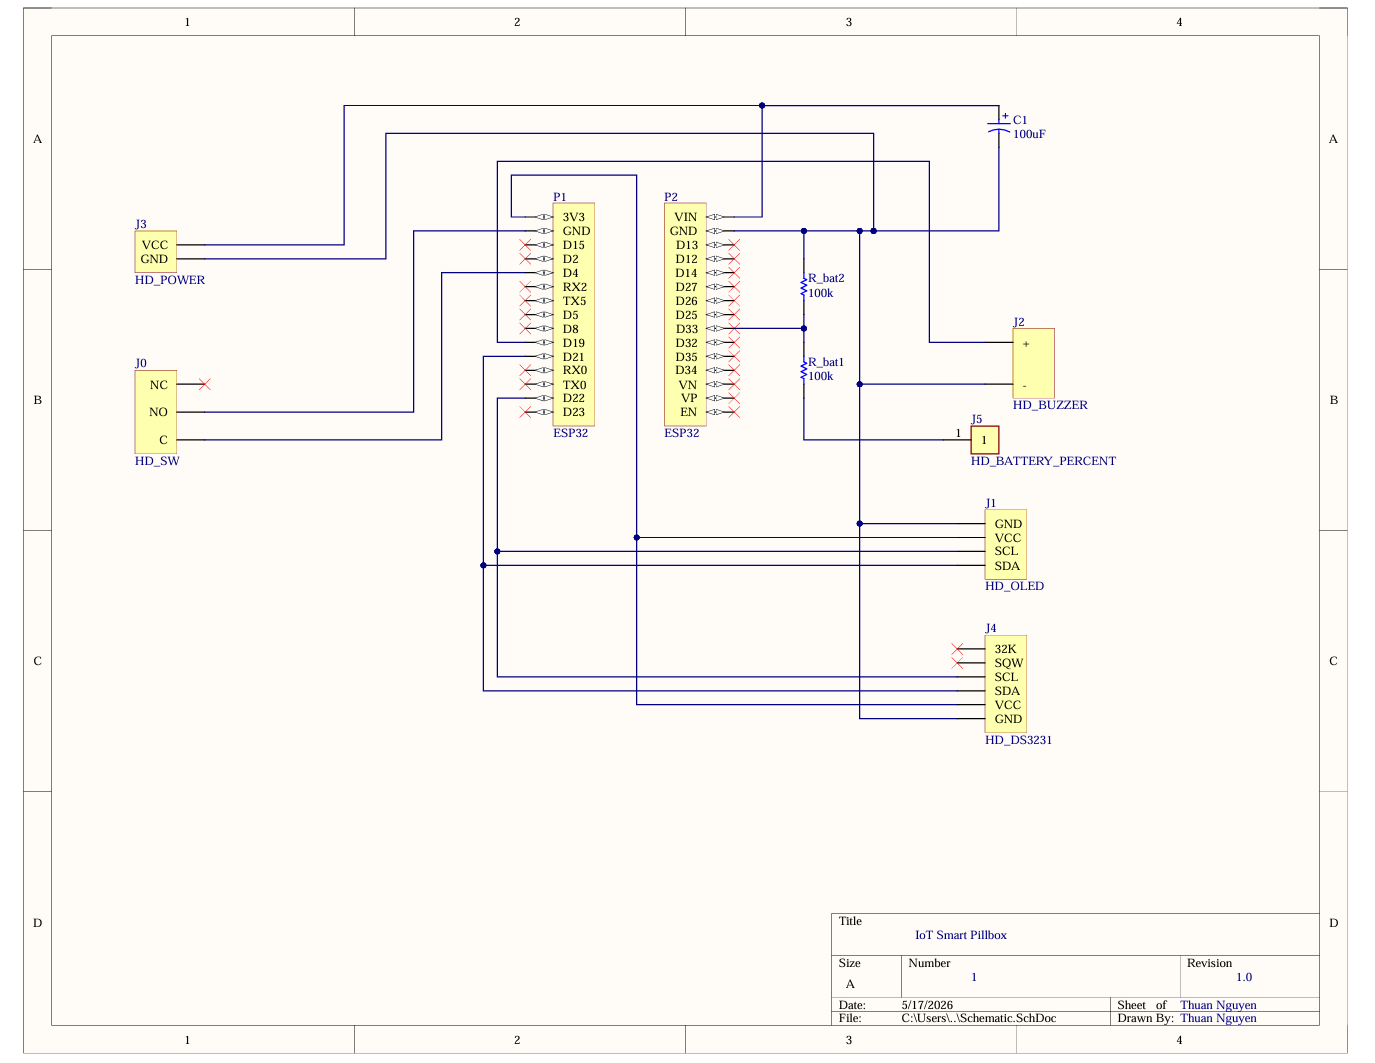
\includegraphics[width=\textwidth]{schematic.png}
    \caption{Sơ đồ nguyên lý hệ thống Hộp Thuốc IoT thiết kế trên Altium Designer}
    \label{fig:schematic}
\end{figure}

Sự phân bổ tín hiệu và tổ chức sơ đồ mạch điện được quy hoạch chi tiết như sau:
\begin{itemize}
    \item \textbf{Cụm kết nối nguồn chính và ổn định áp (J3):} Rào cắm J3 nhận nguồn điện một chiều 5V ổn định từ ngõ ra của module sạc tăng áp. Tại đây, tụ hóa lọc nguồn C1 (100uF) được bố trí song song nối từ đường VCC xuống mass chung để dập nhiễu tần số cao và bù dòng. Nguồn điện sau lọc được đưa trực tiếp vào chân VIN của ESP32 nhằm tận dụng IC ổn áp hạ tầng tuyến tính nội vi của bo mạch để tạo ra nguồn 3.3V cấp cho chip core.
    \item \textbf{Cụm giám sát điện áp đầu vào của pin (J5):} Rào cắm J5 kết nối trực tiếp với cực dương của cell pin di động. Đường tín hiệu này được dẫn qua mạng phân áp gồm điện trở $R_{bat1}$ (100k) và $R_{bat2}$ (100k). Điểm giữa của cầu phân áp trích xuất ra một mức điện áp bằng một nửa áp thực tế của pin, đấu nối trực tiếp vào chân đầu vào tương tự D34 của ESP32 phục vụ hàm thuật toán đo lường dung lượng phần trăm pin.
    \item \textbf{Cụm bus số đồng bộ I2C (J1 và J4):} Rào cắm J1 kết nối màn hình hiển thị OLED và rào cắm J4 kết nối module thời gian thực DS3231 được mắc song song trực tiếp trên cùng một cấu trúc bus I2C. Chân dữ liệu hai chiều SDA kết nối vào chân GPIO21, chân xung nhịp đồng bộ SCL kết nối vào chân GPIO22 của vi điều khiển trung tâm. Toàn bộ các linh kiện trên bus đều được nuôi bằng nguồn 3.3V cấp từ chân ra ổn áp của ESP32 nhằm đảm bảo sự đồng chuẩn về biên độ điện áp logic, chống dòng rò phá hủy cổng đệm.
    \item \textbf{Cụm cơ điện giám sát nắp hộp (J0):} Rào cắm J0 giao tiếp với công tắc hành trình. Chân chung của công tắc nối mass hệ thống, chân thường mở nối trực tiếp vào GPIO15 của ESP32. Chân GPIO15 được lập trình cấu hình kích hoạt điện trở kéo lên nội vi, tạo ra trạng thái tích cực mức thấp ổn định khi nắp hộp bị tác động mở ra.
    \item \textbf{Cụm đầu ra phát cảnh báo (J2):} Rào cắm J2 kết nối còi báo động chủ động, nhận dòng lệnh điều khiển đóng cắt logic trực tiếp từ chân GPIO2 của vi điều khiển trung tâm.
\end{itemize}


\subsection{Thiết kế mạch in (PCB Layout)}
Sau khi hoàn thiện kiểm tra lỗi thiết kế trên sơ đồ nguyên lý, cấu trúc mạch in được triển khai và định hình thực tế. Khác với các sản phẩm công nghiệp đi dây tự động siêu nhỏ, bo mạch của đồ án được tính toán hình học hướng đến khả năng tối ưu cho phương pháp gia công ủi mạch và ăn mòn hóa học thủ công.

\subsubsection{Thiết lập quy tắc thiết kế}
Để đảm bảo bo mạch sau khi ủi nhiệt và ăn mòn bằng dung dịch hóa chất không bị đứt mạch, rỗ đồng hay lem thiếc khi hàn tay, các thông số trong bảng quy tắc thiết kế được thiết lập đặc biệt:
\begin{itemize}
    \item \textbf{Độ rộng đường mạch:} Toàn bộ hệ thống đường đi dây dẫn nguồn chính cũng như các đường truyền tín hiệu đều được đẩy độ rộng lên mức rất lớn, dao động từ \textbf{30 mil đến 35 mil}. Kích thước to bản này đảm bảo lớp mực in bám chắc chắn lên phôi đồng, không bị bong tróc dưới nhiệt độ của bàn là và không bị axit lẹm vào lõi.
    \item \textbf{Khoảng cách an toàn:} Khoảng cách an toàn giữa các đường đồng kề nhau được nới rộng tối đa để tránh hiện tượng mực in bị lem dính vào nhau lúc ủi. Đường kính các chân cắm linh kiện của các rào cắm được tăng kích thước và phủ đồng rộng, giúp chân đồng không bị bong ra khỏi phíp sợi thủy tinh khi chịu tác động nhiệt từ mỏ hàn tay.
    \item \textbf{Phủ đồng tiếp mass toàn phần:} Sử dụng kỹ thuật phủ kín lớp đồng trên phần diện tích trống của mạch và nối với mạng mass chung (GND). Giải pháp này vừa giúp rút ngắn thời gian ăn mòn hóa chất do lượng đồng thừa ít, vừa tạo ra một thảm chắn nhiễu điện từ trường hiệu quả.
\end{itemize}

\subsubsection{Hình ảnh thiết kế thực tế}
Dưới đây là chi tiết bố cục hình học 2D và mô phỏng 3D của bo mạch sau khi đã hoàn thiện quá trình đi dây:

\begin{figure}[H]
    \centering
    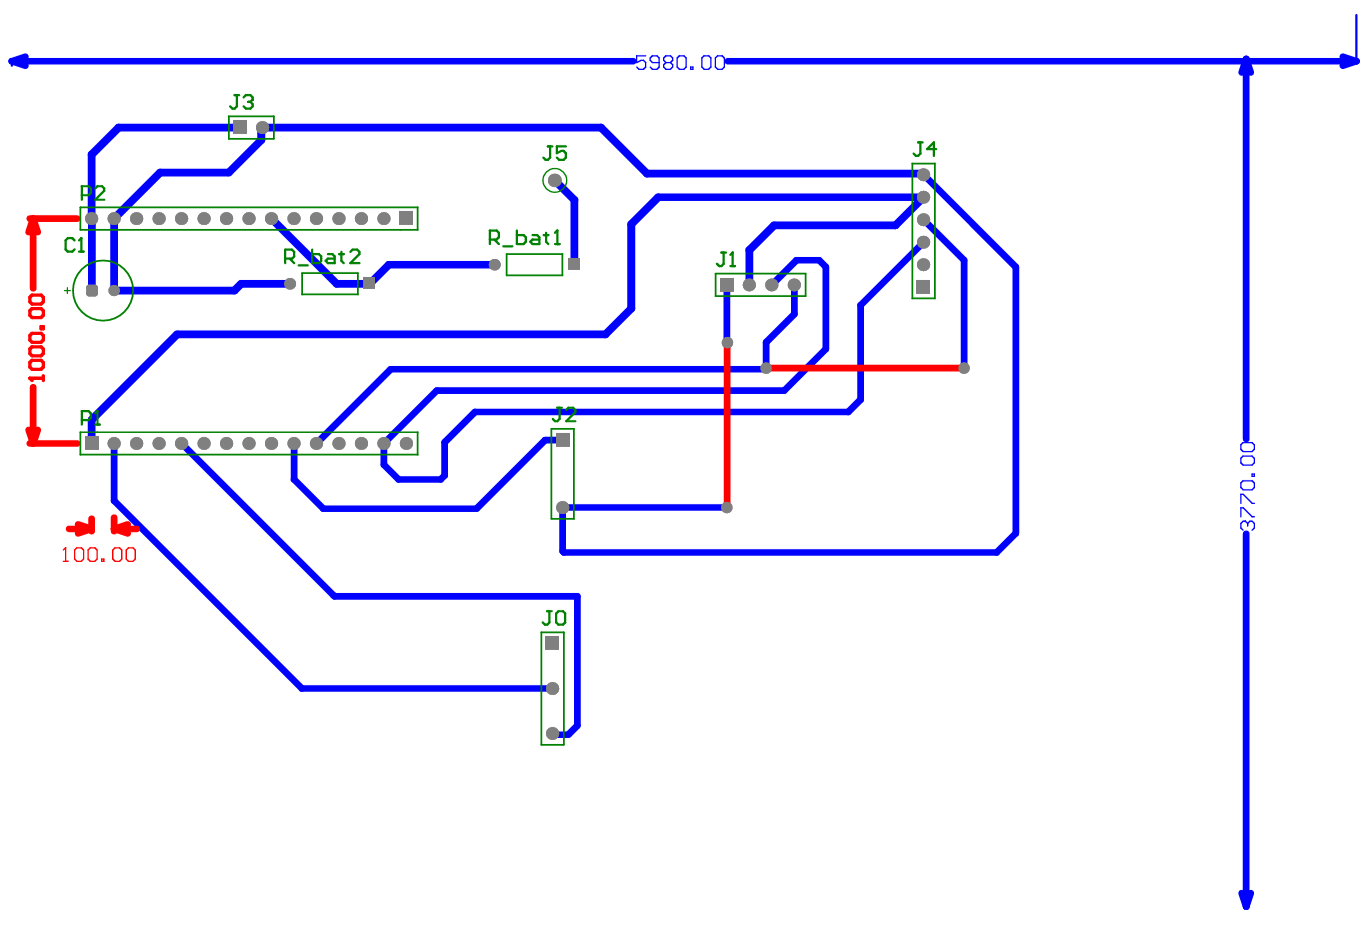
\includegraphics[width=0.75\textwidth]{pcb_2d.png}
    \caption{Thiết kế đường mạch in 2D lớp Bottom với độ rộng vệt đồng 30-35 mil}
    \label{fig:pcb_2d}
\end{figure}

\begin{figure}[H]
    \centering
    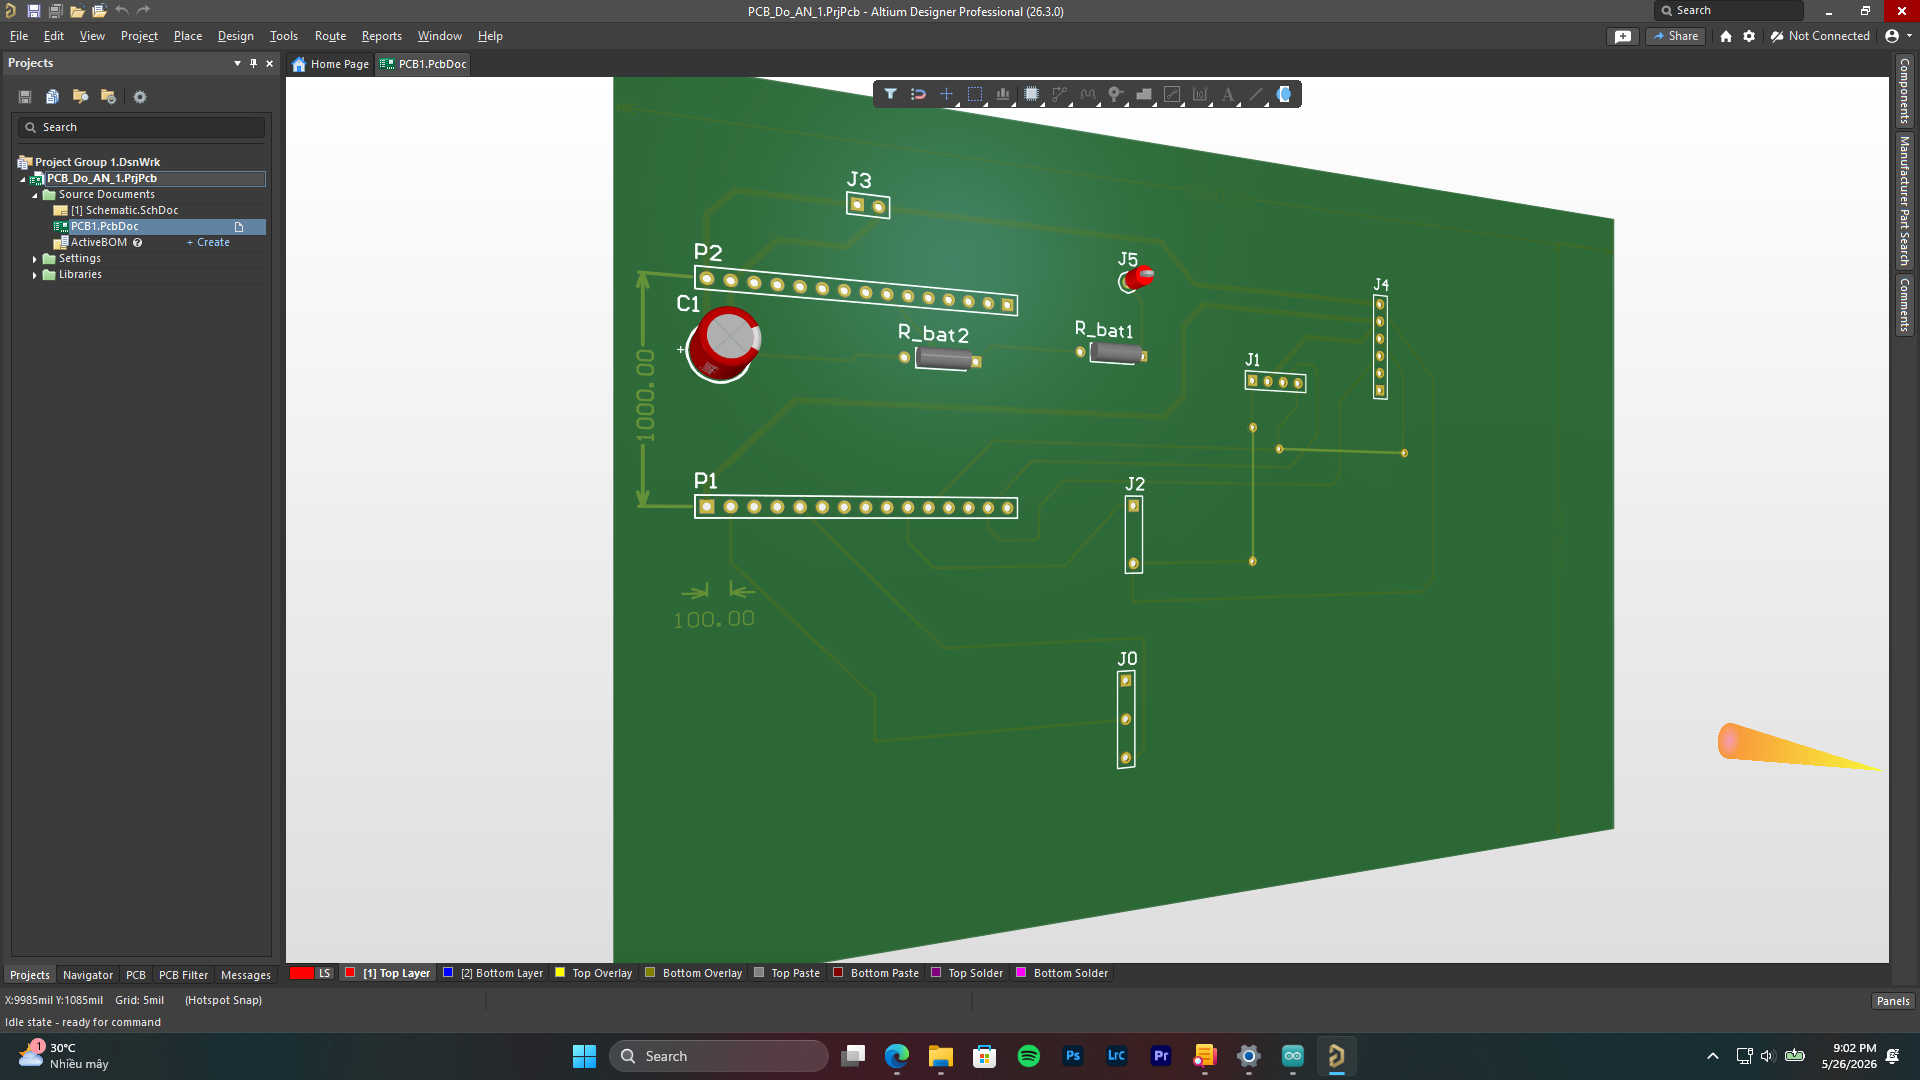
\includegraphics[width=0.75\textwidth]{pcb_3d_front.png}
    \caption{Giao diện mô phỏng hình học 3D mặt trước (Top View) của bo mạch}
    \label{fig:pcb_3d_front}
\end{figure}

\begin{figure}[H]
    \centering
    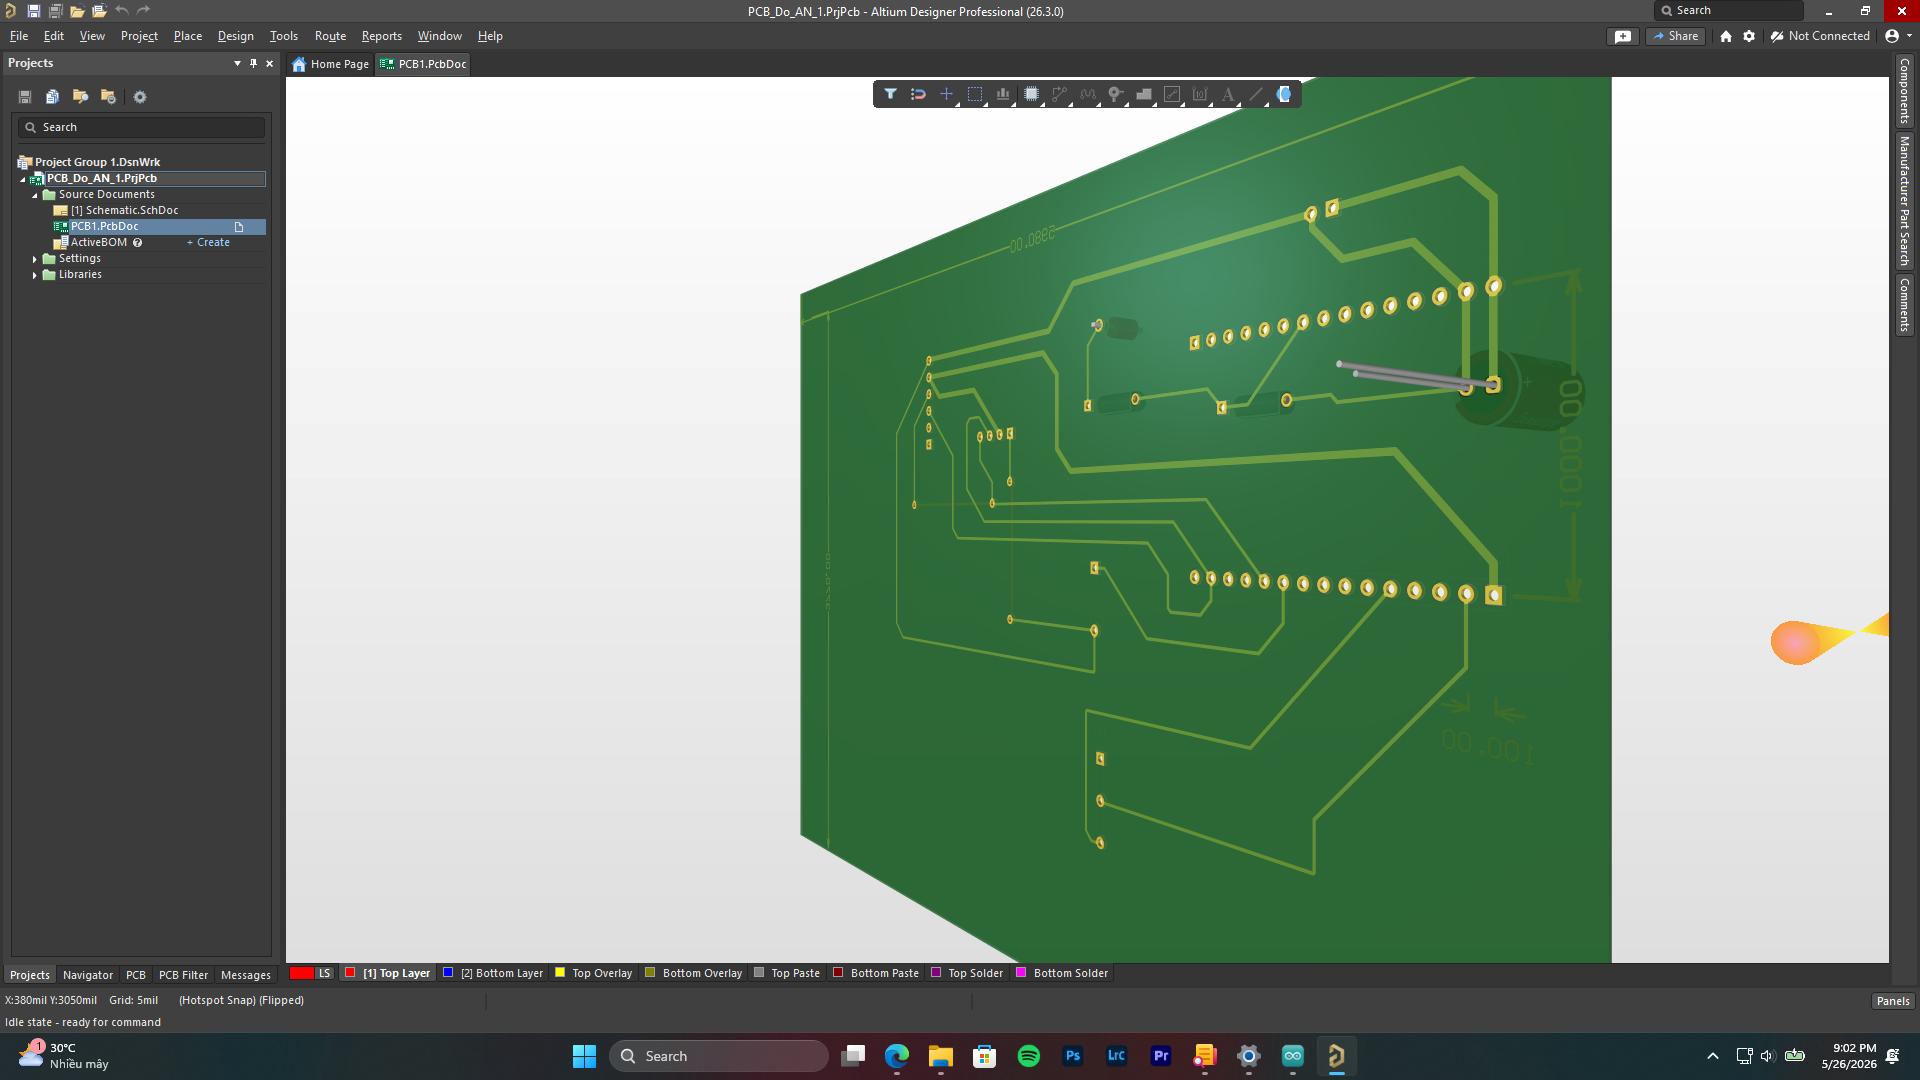
\includegraphics[width=0.75\textwidth]{pcb_3d_back.png}
    \caption{Giao diện mô phỏng hình học 3D mặt sau (Bottom View) thể hiện đường mạch}
    \label{fig:pcb_3d_back}
\end{figure}

\subsubsection{Phân tích thông số kích thước và bố cục linh kiện}
Bo mạch được quy hoạch cấu trúc với kích thước bao tổng thể là 5980 mil × 3770 mil (tương đương khoảng $152\text{ mm} \times 96\text{ mm}$), hoàn toàn khớp với ngàm cố định ở đáy hộp thuốc cơ khí. Chiến thuật sắp xếp linh kiện tuân thủ nghiêm ngặt các nguyên lý động lực học dòng điện và chống nhiễu:
\begin{itemize}
    \item \textbf{Quy hoạch không gian vi điều khiển:} Hai dãy rào cắm đỡ khối ESP32 được bố trí song song ở khu vực trung tâm thiên về bên trái với khoảng cách cách lòng chuẩn xác là 1000 mil (25.4 mm), khớp tuyệt đối với kích thước chân của board Devkit V1, giúp triệt tiêu hoàn toàn ứng suất cơ học gây cong chân linh kiện.
    \item \textbf{Bố trí khối nguồn và lọc nhiễu:} Rào cắm nguồn chính được đặt ở góc trên bên trái, sát ngay vị trí chân cấp nguồn của ESP32. Tụ hóa lọc nguồn 100uF được ưu tiên đặt nằm ngay sát vách chân rào cắm và đường nguồn vào vi điều khiển. Việc ép khoảng cách đường mạch nguồn ngắn nhất giúp triệt tiêu điện trở ký sinh của đường dây đồng, cho phép tụ xả dòng bù áp tức thời với hiệu suất cao nhất.
    \item \textbf{Bố trí khối đo lường pin:} Hai điện trở phân áp 100k được đặt kẹp sát cạnh rào cắm đo áp pin và chân đọc tương tự D34. Việc thu hẹp diện tích đi dây giúp cách ly đường tín hiệu đo lường nhạy cảm khỏi vùng nhiễu tần số cao phát ra từ module nguồn.
    \item \textbf{Bố trí cụm bus số I2C và ngõ ra:} Rào cắm màn hình OLED và đồng hồ DS3231 được gom thành một cụm chức năng ở phía bên phải. Việc đặt sát nhau cho phép đường mạch rẽ nhánh bus I2C ngắn nhất, giảm thiểu điện dung ký sinh trên đường truyền. Rào cắm công tắc hành trình được đẩy hẳn xuống góc dưới cùng bên phải mạch để thuận tiện luồn dây điện ra bản lề cơ khí của nắp hộp thuốc.
    \item \textbf{Chiến thuật đi dây đơn lớp:} Toàn bộ hệ thống đường mạch in đều được đi vát một góc 45 độ, loại bỏ góc vuông 90 độ nhằm chống hiện tượng dội sóng tín hiệu và bẫy axit khi ăn mòn mạch. Toàn bộ các đường tín hiệu được thiết kế chạy liền mạch trên một lớp duy nhất mà không cần sử dụng bất kỳ lỗ xuyên mạch nào, gia tăng độ bền cơ học cho hệ thống.
\end{itemize}

\subsection{Thiết kế cơ khí và vỏ hộp}
\subsubsection{Lựa chọn phôi vỏ hộp và thông số hình học}
Để hiện thực hóa cấu trúc bao che cho sản phẩm một cách nhanh chóng và tối ưu hóa chi phí sản xuất, đề tài lựa chọn giải pháp sử dụng vỏ hộp nhựa kỹ thuật đúc sẵn được phân phối thương mại. Vỏ hộp được chế tạo từ chất liệu nhựa ABS dẻo dai, sở hữu độ bền cơ học cao, khả năng cách điện tuyệt đối và bề mặt nhẵn mịn thẩm mỹ. Với kích thước hình học tổng thể được lựa chọn phù hợp với không gian bo mạch in, vỏ hộp đảm bảo tính nhỏ gọn của một thiết bị y tế cá nhân di động, đồng thời cung cấp cấu trúc nắp đóng mở linh hoạt, tạo điều kiện thuận lợi cho việc bố trí và cơ chế tác động của công tắc hành trình.

\subsubsection{Giải pháp thiết kế phân tầng không gian nội bộ}
Nhằm cách ly hoàn toàn hệ thống linh kiện điện tử nhạy cảm khỏi môi trường lưu trữ y tế và tối ưu hóa diện tích sử dụng, không gian bên trong hộp được quy hoạch theo cơ cấu phân tầng hai lớp thông qua một vách ngăn kỹ thuật nằm ngang:
\begin{itemize}
    \item \textbf{Tầng kỹ thuật phía dưới:} Là nơi định vị cố định bo mạch điều khiển trung tâm và khối pin lưu trữ năng lượng Lithium-Ion. Việc đặt các cấu kiện điện tử và nguồn điện ở đáy hộp giúp hạ thấp trọng tâm vật lý, đảm bảo thiết bị vận hành vững chãi trên mặt phẳng, đồng thời bảo vệ mạch điện khỏi các tác động cơ học trực tiếp từ bên ngoài.
    \item \textbf{Vách ngăn trung gian và cơ chế hành trình:} Một tấm vách ngăn bằng vật liệu nhựa nhẹ được lót ở giữa nhằm che chắn toàn bộ tầng kỹ thuật bên dưới. Tại vị trí bản lề, vách ngăn được khoét một khe hở nhỏ để luồn hệ thống đòn bẩy gạt nảy của công tắc hành trình nhô lên phía trên. Khi nắp hộp đóng lại, nắp sẽ tì đè trực tiếp lên cần gạt công tắc; khi nắp mở ra, công tắc lập tức giải phóng tiếp điểm để kích hoạt luồng dữ liệu cảnh báo.
    \item \textbf{Tầng lưu trữ phía trên:} Toàn bộ khoảng không gian còn lại phía trên vách ngăn được tận dụng làm ngăn chứa thuốc sạch sẽ, thông thoáng. Thiết kế phân tầng này giúp người bệnh dễ dàng lấy thuốc mà không tiếp xúc vật lý với mạch điện, ngăn ngừa hoàn toàn nguy cơ rò rỉ điện hoặc làm hư hỏng các đường dây tín hiệu bên trong.
\end{itemize}

\begin{figure}[H]
    \centering
    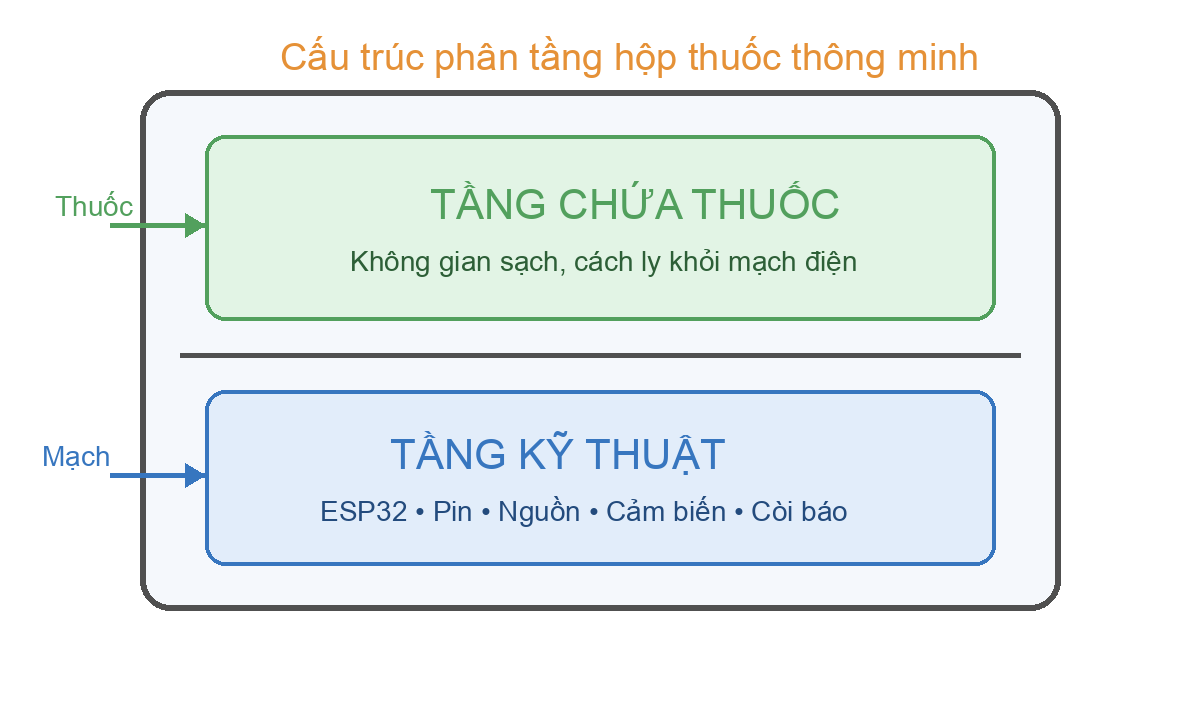
\includegraphics[width=0.65\textwidth]{cau_truc_phan_tang.png}
    \caption{Giải pháp phân tầng với ngăn kỹ thuật phía dưới và không gian chứa thuốc phía trên}
    \label{fig:cau_truc_phan_tang}
\end{figure}

\subsubsection{Gia công cơ khí ngoại vi vỏ hộp}
Quá trình gia công cắt gọt các cổng giao tiếp trên phôi hộp ABS đúc sẵn được thực hiện bằng công cụ mài cắt kỹ thuật số cầm tay, đảm bảo độ chuẩn xác và tính thẩm mỹ cao:
\begin{itemize}
    \item \textbf{Cửa sổ hiển thị mặt trước:} Được khoét một ô trống hình chữ nhật có kích thước tương thích hoàn toàn với khung hiển thị của màn hình hữu cơ tự phát quang, giúp tối ưu hóa góc nhìn cho người dùng.
    \item \textbf{Khe cắm nguồn mặt bên:} Được dũa định hình chính xác tại vị trí hông hộp, cho phép luồn đầu cáp sạc kết nối trực tiếp vào cổng Type-C của vi điều khiển mà không cần mở toàn bộ cấu trúc thiết bị.
    \item \textbf{Hệ thống thoát âm cảnh báo:} Khu vực đối diện khối còi báo động được khoan các lỗ thoát âm biên độ nhỏ, hỗ trợ sóng âm lan tỏa ra môi trường với cường độ định mức cao nhất mà vẫn ngăn chặn được bụi bẩn lọt vào bên trong.
\end{itemize}

\begin{figure}[H]
    \centering
    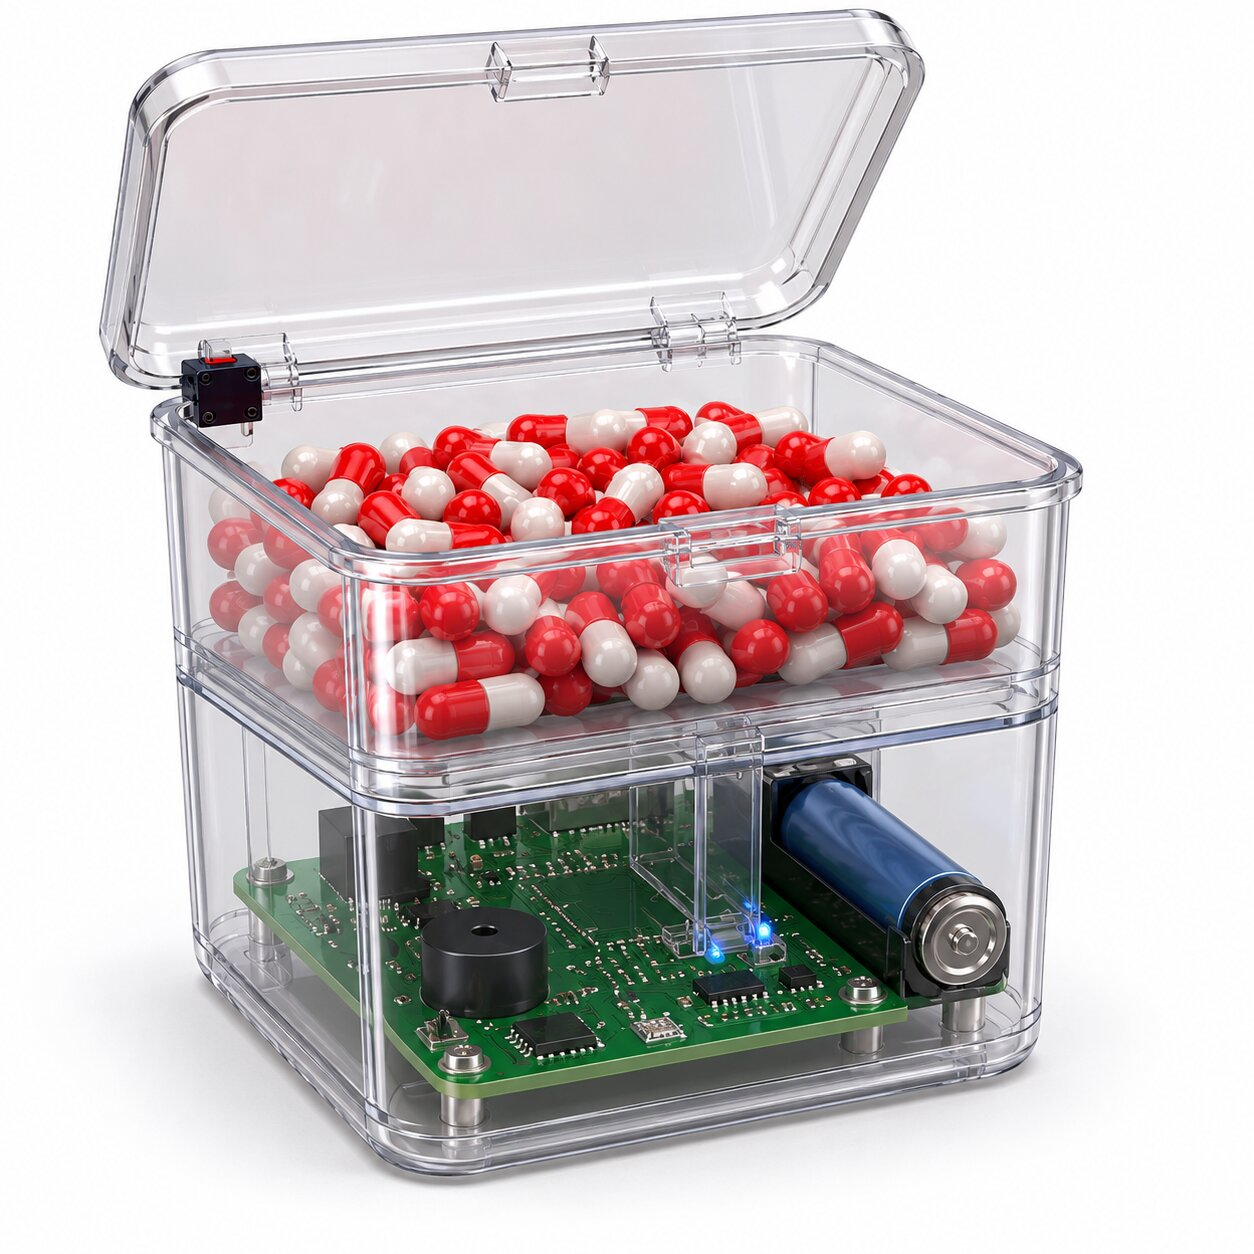
\includegraphics[width=0.65\textwidth]{hop_nhua_hoan_thien.jpg}
    \caption{Ngoại quan tổng thể của hệ thống sau khi hoàn thiện gia công cơ khí trên phôi hộp đúc sẵn (Ảnh minh hoạ)}
    \label{fig:hop_nhua_hoan_thien}
\end{figure}

\subsubsection{Gia công cơ khí và hoàn thiện bề mặt}
Quá trình gia công cơ khí vỏ hộp đòi hỏi độ chính xác cao để đảm bảo tính thẩm mỹ và công năng của thiết bị. Các thao tác cắt gọt được thực hiện bằng công cụ mài cắt đa năng tốc độ cao:
\begin{itemize}
    \item \textbf{Mặt trước:} Được gia công khoét rãnh hình chữ nhật với kích thước chuẩn xác, đóng vai trò làm cửa sổ hiển thị cho màn hình hữu cơ tự phát quang, đảm bảo góc nhìn rộng và không bị lẹm thông tin.
    \item \textbf{Mặt bên:} Được khoan và dũa định hình cửa ngõ giao tiếp cho cổng nạp năng lượng Type-C, cho phép người dùng dễ dàng kết nối bộ sạc mà không cần tháo rời vỏ hộp.
    \item \textbf{Cửa thoát âm:} Vị trí đối diện còi báo động được gia công các lỗ thoát âm nhỏ, giúp sóng âm định hướng khuếch đại ra môi trường bên ngoài mà không làm suy giảm cường độ âm thanh cảnh báo.
\end{itemize}

\begin{figure}[H]
    \centering
    \includegraphics[width=0.65\textwidth]{vo_hop_hoan_thien.jpg} % Bạn chèn ảnh chụp vỏ hộp đã đóng nắp hoàn thiện đẹp đẽ vào đây
    \caption{Tổng thể ngoại quan thiết bị sau khi hoàn thiện gia công cơ khí}
    \label{fig:vo_hop_hoan_thien}
\end{figure}

\subsection{Dự toán kinh phí và Đánh giá hiệu quả kinh tế hệ thống}
\subsubsection{Bảng tổng hợp danh mục vật tư và kinh phí sản xuất}
Để đánh giá tính khả thi về mặt kinh tế và khả năng triển khai thực tiễn của đề tài, toàn bộ chi phí vật tư cấu thành nên một nguyên mẫu thử nghiệm của hệ thống được tổng hợp chi tiết trong Bảng \ref{tab:bom_chiphi}.

\begin{table}[H]
    \centering
    \vspace{0.2cm}
    \renewcommand{\arraystretch}{1.3} % Giãn dòng đảm bảo độ thông thoáng cho bảng dữ liệu
    \resizebox{\textwidth}{!}{% Ép kích thước bảng vừa vặn với chiều rộng văn bản, chống tràn lề vật lý
    \begin{tabular}{|c|l|c|r|r|}
        \hline
        \textbf{STT} & \textbf{Tên linh kiện / Vật tư kỹ thuật} & \textbf{Số lượng} & \textbf{Đơn giá (VNĐ)} & \textbf{Thành tiền (VNĐ)} \\ \hline
        1 & Vi điều khiển cấu trúc lõi kép ESP32 NodeMCU 30-pin & 1 & 125.000 & 125.000 \\ \hline
        2 & Màn hình hiển thị công nghệ OLED I2C SSD1315 & 1 & 47.000 & 47.000 \\ \hline
        3 & Module thời gian thực độc lập DS3231 (kèm nguồn dự phòng) & 1 & 40.000 & 40.000 \\ \hline
        4 & Mạch quản lý nạp và tăng áp tích hợp J5019 & 1 & 30.000 & 30.000 \\ \hline
        5 & Phíp đồng sợi thủy tinh tráng quang phục vụ gia công & 1 & 25.000 & 25.000 \\ \hline
        6 & Vật tư phụ (Rào cắm, dây dẫn tín hiệu, thiếc hàn, công tắc) & 1 & 20.000 & 20.000 \\ \hline
        7 & Còi báo động cấu trúc áp điện chủ động & 1 & 9.000 & 9.000 \\ \hline
        8 & Tụ điện hóa lọc nguồn 100$\mu$F - 16V & 1 & 750 & 750 \\ \hline
        9 & Điện trở màng carbon dán 100k$\Omega$ & 2 & 250 & 500 \\ \hline
        \multicolumn{4}{|r|}{\textbf{TỔNG CHI PHÍ KHÁI TOÁN:}} & \textbf{297.250} \\ \hline
    \end{tabular}%
    }
    \caption{Bảng tổng hợp kinh phí sản xuất nguyên mẫu hệ thống}
    \label{tab:bom_chiphi}
\end{table}

\subsubsection{Phân tích và đánh giá mức chi phí sản xuất sản phẩm}
Dựa trên số liệu thực tế tại Bảng \ref{tab:bom_chiphi}, tổng kinh phí ước tính để hoàn thiện phần cứng cho một đơn vị sản phẩm nguyên mẫu là dưới 300.000 VNĐ. Đối với một hệ thống nhúng có khả năng thực thi các tác vụ mạng phức tạp, đồng bộ hóa thời gian thực và quản lý cơ sở dữ liệu phân tán, mức chi phí này phản ánh sự hợp lý trong việc tính toán và lựa chọn cấu kiện. Các luận điểm kỹ thuật - kinh tế được làm rõ như sau:

\begin{itemize}
    \item \textbf{Tối ưu hóa tài nguyên phần cứng trung tâm:} Thành phần chiếm tỷ trọng ngân sách lớn nhất là vi điều khiển trung tâm ESP32 (xấp xỉ 42\% tổng chi phí). Tuy nhiên, đây là giải pháp tối ưu thay vì lựa chọn các kiến trúc vi điều khiển lõi đơn kết hợp với module thu phát vô tuyến rời. Sự tích hợp này không chỉ giảm thiểu không gian cơ khí mà còn loại bỏ các sai số xung đột giao tiếp dòng dữ liệu, đảm bảo hiệu suất xử lý không đồng bộ của hai tầng tác vụ ứng dụng và truyền thông.
    \item \textbf{Đảm bảo tính độc lập và an toàn dữ liệu y tế:} Khối hiển thị dữ liệu và khối thời gian thực độc lập chiếm khoảng 29\% tổng giá trị cấu thành. Việc duy trì module thời gian thực bù nhiệt là yêu cầu bắt buộc nhằm duy trì hoạt động định thời chính xác kể cả trong kịch bản mất liên lạc mạng toàn phần, bảo vệ tính toàn vẹn của phác đồ điều trị và ngăn ngừa rủi ro trôi giờ báo thức.
    \item \textbf{Ứng dụng giải pháp khai thác năng lượng tuần hoàn:} Bộ nguồn lưu trữ năng lượng từ pin Lithium-Ion không phát sinh chi phí trong danh mục vật tư do đề tài hướng tới việc tận dụng và tái chuẩn hóa các cell pin từ thiết bị di động cũ. Phương án này giúp giảm giá thành hệ thống, đồng thời kiểm chứng khả năng vận hành dòng xả ổn định của các khối năng lượng tái chế trong các hệ thống nhúng công suất thấp.
\end{itemize}

\subsubsection{Chiến lược tối ưu hóa chi phí khi triển khai sản xuất hàng loạt}
Mức chi phí hiện tại được tối ưu cho giai đoạn nghiên cứu và phát triển nguyên mẫu thử nghiệm. Khi chuyển dịch sang giai đoạn thương mại hóa và chế tạo ở quy mô công nghiệp với số lượng lớn, giá thành sản xuất trên một đơn vị thiết bị có thể giảm đáng kể thông qua các giải pháp kỹ thuật chuyên sâu:

\begin{itemize}
    \item \textbf{Tối ưu hóa kiến trúc mạch nguyên khối:} Loại bỏ hoàn toàn việc sử dụng bo mạch phát triển đầu cuối NodeMCU và các module ngoại vi độc lập liên kết qua các cổng rào cắm vật lý. Thiết kế sơ đồ nguyên lý mới sẽ tích hợp trực tiếp chip xử lý hệ thống trên một bo mạch chủ duy nhất. Các linh kiện thụ động và IC quản lý nguồn chuyên dụng như mạch sạc tuyến tính hay mạch chuyển đổi nâng áp chuyển mạch tần số cao sẽ được thiết kế dạng dán bề mặt, giúp tối thiểu hóa kích thước hình học PCB và giảm chi phí nhân công lắp ráp thủ công.
    \item \textbf{Ứng dụng các dòng vi xử lý chuyên biệt giá rẻ:} Thay thế module lõi kép bằng các kiến trúc lõi đơn cấu trúc RISC-V có tích hợp Wi-Fi thế hệ mới, giúp giảm chi phí phôi bán dẫn trung tâm xuống hơn một nửa trong khi vẫn đáp ứng đầy đủ các thuật toán biên mã hóa HTTPS và đẩy dữ liệu đám mây.
    \item \textbf{Tác động từ hiệu ứng quy mô kinh tế:} Khi triển khai đặt hàng cấu kiện bán dẫn, linh kiện thụ động dán và đặt dây chuyền gia công dán mạch tự động với số lượng lớn, chi phí khấu hao thiết kế và đơn giá vật tư đầu vào sẽ giảm theo hình học, cho phép hạ giá thành sản xuất thương mại ước tính xuống dưới 150.000 VNĐ một đơn vị sản phẩm.
\end{itemize}

\newpage
\begin{center}
    \section{THIẾT KẾ VÀ THỰC HIỆN PHẦN MỀM}
\end{center}
%Nội dung chương 4
\subsection{Các thư viện phần mềm cốt lõi và chức năng tích hợp}
Hệ thống phần mềm trên ESP32 được phát triển dựa trên nền tảng Arduino IDE. Để tối ưu hóa quá trình lập trình và tương tác với phần cứng, đề tài sử dụng các thư viện mã nguồn mở chuyên dụng sau:

\begin{itemize}
    \item \textbf{\texttt{WiFiManager.h}:} Thư viện quản lý cấu hình mạng động.
    \begin{itemize}
        \item \textit{Hàm sử dụng:} \texttt{autoConnect()} kích hoạt điểm truy cập cục bộ (AP) và Captive Portal khi rớt mạng, cho phép người dùng nhập mật khẩu Wi-Fi mới mà không cần nạp lại mã nguồn.
    \end{itemize}
    
    \item \textbf{\texttt{WiFiClientSecure.h} \& \texttt{HTTPClient.h}:} Thư viện giao thức vô tuyến.
    \begin{itemize}
        \item \textit{Hàm sử dụng:} \texttt{setInsecure()} bỏ qua xác thực chứng chỉ chuỗi để tiết kiệm RAM. Lệnh \texttt{GET()} và \texttt{POST()} dùng để đóng gói và đẩy/nhận dữ liệu y tế với máy chủ Google Apps Script.
    \end{itemize}
    
    \item \textbf{\texttt{Adafruit\_SSD1306.h} \& \texttt{Adafruit\_GFX.h}:} Thư viện đồ họa màn hình.
    \begin{itemize}
        \item \textit{Hàm sử dụng:} \texttt{display()} xuất bộ đệm nội dung ra màn hình OLED. Hàm \texttt{ssd1306\_command()} dùng để can thiệp trực tiếp vào thanh ghi ép xung giảm sáng (Deep Dimming).
    \end{itemize}
    
    \item \textbf{\texttt{RTClib.h}:} Thư viện giao tiếp đồng hồ thời gian thực DS3231.
    \begin{itemize}
        \item \textit{Hàm sử dụng:} \texttt{now()} trích xuất thời gian hiện tại để hiển thị. Hàm \texttt{setAlarm1()} nạp cấu hình cữ thuốc vào thanh ghi để sinh ngắt phần cứng.
    \end{itemize}
    
    \item \textbf{\texttt{Preferences.h}:} Thư viện quản lý bộ nhớ tĩnh (Non-Volatile Storage).
    \begin{itemize}
        \item \textit{Hàm sử dụng:} \texttt{begin()} khởi tạo phân vùng nhớ Flash. Hàm \texttt{putString()} và \texttt{getString()} dùng để ghi/đọc mảng dữ liệu lịch sử uống thuốc khi hệ thống bị mất kết nối Wi-Fi.
    \end{itemize}
    
    \item \textbf{\texttt{NTPClient.h}:} Thư viện giao thức đồng bộ thời gian mạng.
    \begin{itemize}
        \item \textit{Hàm sử dụng:} \texttt{update()} và \texttt{getEpochTime()} dùng để kéo mốc thời gian chuẩn từ máy chủ \texttt{pool.ntp.org} về bù trừ sai số cho mạch DS3231 mỗi khi thiết bị trực tuyến.
    \end{itemize}
\end{itemize}



\subsection{Lưu đồ giải thuật hàm khởi tạo (Setup)}

Hàm khởi tạo được thực hiện một lần duy nhất khi thiết bị được cấp nguồn. Trọng tâm của thuật toán này là Cơ chế ưu tiên ngoại tuyến. Thiết bị sẽ luôn trích xuất lịch trình cũ từ bộ nhớ Flash trước khi thử kết nối mạng. Điều này đảm bảo hệ thống vẫn hoạt động trơn tru (dựa trên dữ liệu cũ) ngay cả khi không có kết nối Wi-Fi.

\begin{figure}[H]
    \centering
    \begin{tikzpicture}[
   scale=0.8,             % Thu nhỏ còn 70% kích thước gốc
    transform shape,       % Bắt buộc phải có để các node và chữ thu nhỏ theo
    node distance=1.2cm,   % Giảm khoảng cách giữa các khối
        >=stealth,
        font=\sffamily\small,
        % Định dạng các khối
        startstop/.style={rectangle, rounded corners=15pt, draw=black, thick, fill=gray!20, minimum width=3.5cm, minimum height=0.8cm, text centered, font=\bfseries},
        decision/.style={diamond, aspect=2.5, draw=black, thick, fill=yellow!10, text width=3cm, text centered, inner sep=0pt},
        process/.style={rectangle, draw=black, thick, fill=blue!5, text width=7.5cm, align=left, minimum height=1cm, inner sep=6pt},
        highlight/.style={rectangle, draw=black, thick, fill=green!10, text width=7.5cm, align=left, minimum height=1cm, inner sep=6pt},
        arrow/.style={thick, ->},
        line/.style={thick}
    ]

    % --- 1. KHAI BÁO CÁC KHỐI ---
    \node[startstop] (start) {Setup};

    \node[process, below=0.8cm of start] (proc1) {
        \textbf{Khởi tạo phần cứng:}\\
        - Cấu hình chân I/O \\
        - Bật giao tiếp I2C
    };

    % Khối nhấn mạnh việc đọc Flash trước khi kết nối mạng
    \node[highlight, below=0.8cm of proc1] (proc2) {
        \textbf{Khôi phục dữ liệu dự phòng:}\\
        - Đọc lịch uống thuốc lưu sẵn trong Flash
    };

    % BỔ SUNG KHỐI KHỞI TẠO WIFI Ở ĐÂY
    \node[process, below=0.8cm of proc2] (wifi_init) {
        \textbf{Khởi tạo kết nối mạng:}\\
        - Bắt đầu kết nối Wi-Fi \\
        - Khởi động bộ đếm thời gian chờ
    };

    \node[decision, below=0.8cm of wifi_init] (dec1) {Kết nối Wi-Fi\\thành công?};

    % Nhánh Online
    \node[process, right=1.5cm of dec1] (proc_online) {
        \textbf{Chế độ Online (Cập nhật mới):}\\
        - Đồng bộ giờ NTP cập nhật RTC\\
        - Tải lịch mới nhất từ máy chủ Cloud
    };

    % Nhánh Offline
    \node[process, fill=orange!10, below=0.8cm of dec1] (proc_offline) {
        \textbf{Chế độ Offline (Sự cố mạng):}\\
        - Bỏ qua mạng, hoạt động\\
        bằng lịch cũ đã nạp từ Flash
    };

    \node[startstop, below=0.8cm of proc_offline] (end) {Kết thúc Setup};

    % --- 2. VẼ ĐƯỜNG MŨI TÊN CHÍNH ---
    \draw[arrow] (start) -- (proc1);
    \draw[arrow] (proc1) -- (proc2);
    \draw[arrow] (proc2) -- (wifi_init);
    \draw[arrow] (wifi_init) -- (dec1);

    % Nhánh Đúng (Sang phải)
    \draw[arrow] (dec1) -- node[above, font=\scriptsize] {Đúng} (proc_online);
    
    % Nhánh Sai (Đi thẳng xuống)
    \draw[arrow] (dec1) -- node[left, font=\scriptsize] {Sai / Hết thời gian chờ} (proc_offline);

    % Về đích
    \draw[arrow] (proc_offline) -- (end);

    % Đường gộp từ nhánh Online xuống đích (Vẽ đường chữ L)
    \draw[arrow] (proc_online.south) |- (end.east);

    \end{tikzpicture}
    \caption{Trình tự khởi tạo hệ thống, nhấn mạnh cơ chế xử lý ngoại tuyến (Offline)}
    \label{fig:luu_do_setup}
\end{figure}


\subsection{Lưu đồ giải thuật vòng lặp chính (Main Loop)}

Thuật toán của hệ thống được thiết kế theo kiến trúc Non-blocking, sử dụng bộ đếm thời gian thực để chia sẻ tài nguyên CPU cho 4 luồng độc lập. Lưu đồ Hình \ref{fig:luu_do_loop} mô tả logic xử lý của hệ thống bằng ngôn ngữ tự nhiên, tập trung vào bản chất luồng dữ liệu thay vì các dòng lệnh phức tạp, giúp người đọc dễ dàng nắm bắt nguyên lý hoạt động:

\begin{figure}[H]
    \centering
    \begin{tikzpicture}[
        node distance=1.2cm and 1.5cm,
        >=stealth,
        font=\sffamily\small,
        % Định dạng các khối
        startstop/.style={rectangle, rounded corners=15pt, draw=black, thick, fill=gray!20, minimum width=3cm, minimum height=0.8cm, text centered, font=\bfseries},
        decision/.style={diamond, aspect=2.5, draw=black, thick, fill=yellow!10, text width=3cm, text centered, inner sep=0pt},
        process/.style={rectangle, draw=black, thick, fill=blue!5, text width=5cm, align=left, minimum height=1cm, inner sep=6pt},
        arrow/.style={thick, ->},
        line/.style={thick}
    ]

    % --- 1. KHAI BÁO CÁC KHỐI ---
    \node[startstop] (start) {Bắt đầu vòng lặp};

    % Task 1
    \node[decision, below=0.8cm of start] (dec1) {Đủ chu kỳ 1 giây?};
    \node[process, right=1.5cm of dec1] (proc1) {
        - Cập nhật giờ lên OLED\\
        - Quét danh sách báo thức
    };

    % Task 2
    \node[decision, below=1cm of dec1] (dec2) {Đang có báo thức?};
    \node[process, right=1.5cm of dec2] (proc2) {
        - Phát xung Buzzer\\
        - Nếu > 5 phút: Ghi "Bỏ cữ"
    };

    % Task 3
    \node[decision, below=1cm of dec2] (dec3) {Trạng thái nắp sau 30p?};
    \node[process, right=1.5cm of dec3] (proc3) {
        - Mở: Ghi "Uống trễ"\\
        - Đóng: Ghi "Đóng nắp"
    };

    % Task 4
    \node[decision, below=1cm of dec3] (dec4) {Đến hạn đồng bộ?};
    \node[process, right=1.5cm of dec4] (proc4) {
        - Tải lịch mới từ Cloud
    };

    % Điểm neo kết thúc
    \node[coordinate, below=0.8cm of dec4] (end) {};

    % --- 2. VẼ ĐƯỜNG TRỤC CHÍNH (XUỐNG DƯỚI) ---
    \draw[arrow] (start) -- (dec1);
    \draw[arrow] (dec1) -- node[left, font=\scriptsize] {Sai} (dec2);
    \draw[arrow] (dec2) -- node[left, font=\scriptsize] {Sai} (dec3);
    \draw[arrow] (dec3) -- node[left, font=\scriptsize] {Sai} (dec4);
    \draw[line]  (dec4) -- node[left, font=\scriptsize] {Sai} (end);

    % --- 3. VẼ ĐƯỜNG NHÁNH (SANG PHẢI) ---
    \draw[arrow] (dec1) -- node[above, font=\scriptsize] {Đúng} (proc1);
    \draw[arrow] (dec2) -- node[above, font=\scriptsize] {Đúng} (proc2);
    \draw[arrow] (dec3) -- node[above, font=\scriptsize] {Đúng} (proc3);
    \draw[arrow] (dec4) -- node[above, font=\scriptsize] {Đúng} (proc4);

    % --- 4. VẼ ĐƯỜNG GỘP TRỞ LẠI TRỤC CHÍNH ---
    \draw[arrow] (proc1.south) |- ($(dec1.south)!0.5!(dec2.north)$);
    \draw[arrow] (proc2.south) |- ($(dec2.south)!0.5!(dec3.north)$);
    \draw[arrow] (proc3.south) |- ($(dec3.south)!0.5!(dec4.north)$);
    \draw[arrow] (proc4.south) |- (end);

    % --- 5. VẼ ĐƯỜNG LẶP LẠI (VÒNG SANG TRÁI MỘT KHOẢNG RỘNG) ---
    \draw[arrow] (end) -- ++(-3.5,0) |- node[right, pos=0.25, font=\scriptsize\itshape] {Lặp lại liên tục} (start.west);

    \end{tikzpicture}
    \caption{Lưu đồ giải thuật các luồng xử lý bên trong vi điều khiển ESP32}
    \label{fig:luu_do_loop}
\end{figure}

\subsection{Giải thuật tối ưu hóa năng lượng màn hình (Deep Dimming)}
Để kéo dài thời lượng pin cho hệ thống, đồ án triển khai giải thuật điều chế độ sáng mờ tầng sâu (Deep Dimming) cho khối hiển thị OLED thay vì chỉ giảm độ tương phản bằng phần mềm thông thường. Giải thuật can thiệp trực tiếp vào các thanh ghi phần cứng của IC SSD1306 nhằm ép dòng điện rò rỉ về mức tối thiểu khi thiết bị rảnh rỗi.

\textbf{Cơ chế can thiệp phần cứng:}
\begin{itemize}
    \item \textbf{Thanh ghi tiền nạp điện tích (Pre-charge Period - 0xD9):} Ép chu kỳ nạp mồi của tụ ký sinh trên điểm ảnh xuống mức thấp nhất (0x11), triệt tiêu hoàn toàn sự tiêu hao năng lượng từ pha nạp mồi điện áp.
    \item \textbf{Thanh ghi điện áp nền (VCOMH Deselect Level - 0xDB):} Điều chỉnh điện áp phân cực của các đường quét dòng rảnh rỗi về 0, loại bỏ dòng rò trên các pixel không được kích hoạt.
    \item \textbf{Thanh ghi độ sáng (Contrast Control - 0x81):} Khống chế dòng định thiên về mức 0, duy trì độ phản xạ lờ mờ vừa đủ đọc trong bóng râm.
\end{itemize}

\textbf{Logic vận hành trong hệ thống:}
Giải thuật sử dụng bộ định thời \texttt{millis()} để giám sát tương tác vật lý. Nếu sau 30 giây hệ thống không ghi nhận trạng thái mở nắp hoặc báo thức, vi điều khiển lập tức nạp chuỗi lệnh Deep Dimming, kéo dòng tiêu thụ của màn hình từ $\sim 20$mA xuống ngưỡng dưới $2$mA. Ngược lại, khi phát hiện tín hiệu từ công tắc hành trình hoặc RTC, các thông số định mức được tái nạp, đưa màn hình bừng sáng 100\% ngay lập tức để phục vụ cảnh báo y tế.

\subsection{Giao tiếp và Quản lý dữ liệu qua Google Sheets}

Hệ thống ứng dụng kiến trúc Serverless, trong đó Google Sheets đóng vai trò là một Cơ sở dữ liệu (Database) và Google Apps Script (GAS) đóng vai trò là Application Programming Interface (API) Backend để xử lý logic nội bộ.

\subsubsection{Thuật toán ghi nhận sự kiện cơ bản}
Khi có các sự kiện vật lý xảy ra, vi điều khiển ESP32 gửi yêu cầu \texttt{HTTP GET} kèm các tham số hành động (\texttt{action=Mo\_Nap}, \texttt{Bo\_Thuoc},...) lên GAS. Máy chủ sẽ tự động trích xuất dấu thời gian thực (Timestamp) theo múi giờ GMT+7 và ghi nối tiếp (appendRow) vào bảng tính. 

\subsubsection{Thuật toán phân tích ngoại lệ (Logic "Uống trễ")}
Đây là một trong những điểm nhấn kỹ thuật của phần mềm. Trong thực tế, bệnh nhân có thể quên uống thuốc đúng giờ, nhưng lại nhớ ra và uống bù sau đó vài chục phút. Nếu chỉ ghi nhận máy móc, dữ liệu sẽ bị rời rạc. Để khắc phục, một thuật toán "Cửa sổ thời gian quy hồi" được triển khai trên máy chủ GAS:
\begin{enumerate}
    \item Khi nhận được lệnh \texttt{Uong\_Tre} từ thiết bị, GAS không ghi ngay dòng mới mà kích hoạt vòng lặp quét ngược cơ sở dữ liệu từ dưới lên trên.
    \item Thuật toán tìm kiếm dòng trạng thái "Bỏ thuốc" gần nhất. Tại dòng này, chuỗi văn bản thời gian được bóc tách (Parse) ngược trở lại thành đối tượng \texttt{Date} tiêu chuẩn.
    \item Hệ thống tính toán độ lệch thời gian ($\Delta t$) giữa thời điểm hiện tại và mốc báo "Bỏ thuốc". Nếu $\Delta t \le 60$ phút (3.600.000 ms), hệ thống sẽ \textbf{Ghi đè (Overwrite)} trực tiếp lên dòng dữ liệu cũ, đổi trạng thái thành "Uống trễ" và cập nhật lại mốc giờ uống thực tế.
\end{enumerate}
Cơ chế này giúp làm sạch dữ liệu nhiễu, cung cấp cho bác sĩ một báo cáo tuân thủ y tế chính xác nhất.

\begin{figure}[H]
    \centering
    \begin{tikzpicture}[
        node distance=1.2cm and 1.2cm,
        >=stealth,
        font=\sffamily\small,
        % Định dạng các khối
        startstop/.style={rectangle, rounded corners=15pt, draw=black, thick, fill=gray!20, minimum width=3cm, minimum height=0.8cm, text centered, font=\bfseries},
        decision/.style={diamond, aspect=2, draw=black, thick, fill=yellow!10, text width=2.8cm, text centered, inner sep=0pt, font=\scriptsize},
        process/.style={rectangle, draw=black, thick, fill=blue!5, text width=4.2cm, align=left, minimum height=1cm, inner sep=6pt, font=\scriptsize},
        arrow/.style={thick, ->},
        line/.style={thick}
    ]

    % --- 1. KHAI BÁO CÁC KHỐI ---
    \node[startstop] (start) {action = "Uong\_Tre"};

    \node[process, below=0.8cm of start] (read) {Tải toàn bộ dữ liệu Sheet vào mảng 2 chiều (Data Array)};

    \node[process, fill=orange!10, below=0.8cm of read] (loop) {\textbf{Vòng lặp (Bottom-Up):}\\ Quét ngược từ dòng cuối cùng lên dòng 1};

    \node[decision, below=0.8cm of loop] (dec_status) {Cột B có bằng\\ "Bỏ thuốc"?};

    \node[decision, right=1cm of dec_status] (dec_time) {Khoảng cách $\Delta t \le 60$ phút?};

    \node[process, right=1cm of dec_time] (overwrite) {\textbf{Hành động Ghi đè:}\\ 1. Đổi "Bỏ thuốc" $\rightarrow$ "Uống trễ"\\ 2. Cập nhật mốc giờ uống bù\\ 3. Break (Thoát vòng lặp)};

    \node[process, below=1cm of dec_status] (append) {\textbf{Hành động Thêm mới:}\\ (Kết thúc lặp không tìm thấy)\\ Thêm 1 dòng log "Uống trễ" mới ở cuối bảng};

    \node[process, fill=green!10, below=0.8cm of overwrite] (push) {\textbf{Push Notification:}\\ Gửi thông báo [INFO] về Telegram Bot};

    \node[startstop, right=1.5cm of append, yshift=-2cm] (end) {Trả về trạng thái SUCCESS};

    % --- 2. VẼ ĐƯỜNG MŨI TÊN ---
    \draw[arrow] (start) -- (read);
    \draw[arrow] (read) -- (loop);
    \draw[arrow] (loop) -- (dec_status);

    % Nhánh xử lý trạng thái
    \draw[arrow] (dec_status) -- node[above, font=\scriptsize] {Đúng} (dec_time);
    \draw[line] (dec_status.west) -- ++(-1,0) |- node[right, pos=0.25, font=\scriptsize\itshape] {Sai (Duyệt dòng trên)} (loop.west);

  % Nhánh xử lý thời gian
    \draw[arrow] (dec_time) -- node[above, font=\scriptsize] {Đúng} (overwrite);
    \draw[arrow] (dec_time.north) |- node[above, pos=0.75, font=\scriptsize\itshape] {Sai (Bỏ qua)} (loop.east);

    % Thoát vòng lặp thất bại
    \draw[arrow] (dec_status) -- node[left, font=\scriptsize] {Duyệt hết mảng} (append);

    % Gộp luồng về đích
    \draw[arrow] (overwrite) -- (push);
    \draw[arrow] (push) |- (end);
    \draw[arrow] (append) -- (end);

    \end{tikzpicture}
    \caption{Lưu đồ thuật toán xử lý ngoại lệ "Uống trễ" (Tìm kiếm ngược Bottom-Up)}
    \label{fig:uong_tre_flow}
\end{figure}

\subsection{Cơ chế lưu trữ dữ liệu ngoại tuyến vào bộ nhớ tĩnh}
Để đảm bảo tính toàn vẹn của dữ liệu giám sát y tế trong kịch bản mất kết nối mạng toàn phần, hệ thống triển khai một cơ chế lưu trữ hàng đợi ngoại tuyến dựa trên phân vùng bộ nhớ tĩnh không bốc hơi của vi điều khiển. 

\textbf{Cơ chế đóng gói và tổ chức hàng đợi lưu trữ:}
Khi tiến trình gửi dữ liệu lên điện toán đám mây phát hiện trạng thái mất liên lạc vô tuyến, vi điều khiển lập tức chuyển hướng dòng dữ liệu sang chế độ dự phòng. Thông tin về hành vi tương tác cùng dấu mốc thời gian thực hiện hành lấy từ mạch định thời độc lập được ghép nối thành một cấu trúc đồng bộ. Chuỗi dữ liệu này được ghi trực tiếp vào phân vùng bộ nhớ tĩnh của chip dưới dạng các cặp khóa và giá trị định danh. Hệ thống duy trì một biến đếm lưu giữ số lượng bản ghi tồn đọng, đóng vai trò điều hướng chỉ số để xếp chồng các sự kiện theo tuần tự thời gian, ngăn ngừa hiện tượng ghi đè làm mất mát dữ liệu của người bệnh.

\textbf{Logic giải tỏa hàng đợi khi phục hồi kết nối:}
Trong chu kỳ quét của vòng lặp hệ thống, trạng thái liên lạc vô tuyến được giám sát liên tục. Ngay khi mạng Internet được tái lập và xác thực ổn định, vi điều khiển sẽ kích hoạt tiến trình giải phóng bộ nhớ đệm. Hệ thống thực hiện đọc tuần tự các bản ghi từ bộ nhớ tĩnh theo chỉ số từ cũ nhất đến mới nhất để đồng bộ hóa ngược lên máy chủ trang tính. Sau khi nhận được tín hiệu phản hồi xác nhận lưu trữ thành công từ đám mây, vi điều khiển tiến hành xóa sạch phân vùng dữ liệu phụ, đồng thời hoàn tác biến đếm hàng đợi về mức số không để giải phóng hoàn toàn không gian nhớ cho các chu kỳ rớt mạng tiếp theo.

\subsection{Hệ thống tương tác hai chiều qua Telegram Bot}

Thay vì chỉ gửi cảnh báo một chiều, nền tảng Telegram Bot trong đồ án được thiết kế để hoạt động song công (Full-duplex), vừa đóng vai trò là \textit{Hệ thống Cảnh báo (Push)} vừa là \textit{Cổng Truy vấn Thống kê (Pull)}.

\subsubsection{Cơ chế Cảnh báo Chủ động (Push Notifications)}
Quá trình gửi tin nhắn không đi trực tiếp từ mạch lên Telegram nhằm giảm tải mã hóa cho ESP32. Khi máy chủ GAS xử lý xong các lệnh ghi log vào Google Sheets, nó sẽ đồng thời gọi phương thức \texttt{UrlFetchApp} tới API của Telegram để đẩy thông báo về điện thoại người nhà.

\textbf{Cấu trúc mã tạo tin nhắn trên máy chủ:}
\begin{verbatim}
var message = "<b>[!] CẢNH BÁO CHƯA UỐNG THUỐC</b>\n" +
              "----------------------------\n" +
              " <b>Thời gian:</b> " + currentTimestampStr + "\n" +
              "<i>Bệnh nhân bỏ lỡ một cữ thuốc! Vui lòng kiểm tra.</i>";
\end{verbatim}
Các tin nhắn sử dụng chuẩn định dạng HTML của Telegram để in đậm (\texttt{<b>}) thông tin then chốt. Sự kiện "Bỏ thuốc" sử dụng ký hiệu cảnh báo \texttt{[!]}, trong khi sự kiện "Mở nắp" đúng giờ sử dụng ký hiệu xác nhận \texttt{[OK]}.

\subsubsection{Cơ chế Webhook Truy vấn Dữ liệu (Pull Requests)}
Để người nhà có thể kiểm tra tình trạng uống thuốc bất cứ lúc nào mà không cần mở trình duyệt, hệ thống thiết lập một kết nối \textbf{Webhook} định tuyến trực tiếp từ máy chủ Telegram về hàm \texttt{doPost(e)} của Google Apps Script.

\begin{figure}[H]
    \centering
    \begin{tikzpicture}[
        node distance=1.8cm,
        >=stealth,
        font=\sffamily\small,
        startstop/.style={rectangle, rounded corners=12pt, draw=black, thick, fill=gray!20, minimum width=6cm, minimum height=0.8cm, text centered, font=\bfseries},
        process/.style={rectangle, draw=black, thick, fill=green!10, text width=6.2cm, inner sep=8pt}
    ]

    % 1. Khai báo các khối (Xếp thẳng hàng dọc)
    \node[startstop] (user) {Người dùng (App Telegram)};
    \node[startstop, below=1.5cm of user] (tele) {Máy chủ Telegram (Bot API)};
    
    % Khối GAS được tích hợp lời diễn giải ở nửa dưới
    \node[process, below=1.5cm of tele] (gas) {
        \centering \bfseries Google AppsScript (Hàm doPost)\\[1ex]
        \hrule\vspace{1ex}
        \raggedright \normalfont \footnotesize
        - Bóc tách lệnh từ JSON payload\\
        - Kích hoạt thuật toán thống kê mảng\\
        - Định dạng kết quả thành chuỗi Text
    };
    
    \node[startstop, below=1.5cm of gas] (sheet) {Cơ sở dữ liệu (Google Sheets)};

    % 2. Vẽ các đường mũi tên (Đã thu hẹp khoảng cách xshift=1.0cm)
    % LƯỢT ĐI (Mũi tên đi xuống, nằm bên phải)
    \draw[->, thick] ([xshift=1.0cm]user.south) -- node[right, align=left] {1. Gửi lệnh (\texttt{/homnay})} ([xshift=1.0cm]tele.north);
    
    \draw[->, thick] ([xshift=1.0cm]tele.south) -- node[right, align=left] {2. Webhook Trigger} ([xshift=1.0cm]gas.north);
    
    \draw[->, thick] ([xshift=1.0cm]gas.south) -- node[right, align=left] {3. Truy xuất \& Ghi log} ([xshift=1.0cm]sheet.north);

    % LƯỢT VỀ (Mũi tên đi lên, nằm bên trái)
    \draw[->, thick] ([xshift=-1.0cm]sheet.north) -- node[left, align=right] {4. Trả kết quả thống kê} ([xshift=-1.0cm]gas.south);
    
    \draw[->, thick] ([xshift=-1.0cm]gas.north) -- node[left, align=right] {5. API \texttt{sendMessage}} ([xshift=-1.0cm]tele.south);
    
    \draw[->, thick] ([xshift=-1.0cm]tele.north) -- node[left, align=right] {6. Hiển thị tin nhắn} ([xshift=-1.0cm]user.south);

    \end{tikzpicture}
    \caption{Lưu đồ quá trình xử lý lệnh tương tác hai chiều qua Webhook}
    \label{fig:telegram_webhook}
\end{figure}

Hệ thống hỗ trợ các tập lệnh tra cứu thông minh như \texttt{/homnay}, \texttt{/tuannay}, \texttt{/thangnay}. Khi nhận được lệnh, hàm \texttt{doPost} sẽ tính toán ngay lập tức tỷ lệ tuân thủ, số lần uống, số lần bỏ lỡ trong khoảng thời gian tương ứng và phản hồi về khung chat chỉ trong vòng dưới 2 giây.

Bên cạnh hàm \texttt{doPost()} chịu trách nhiệm xử lý các yêu cầu từ cấu trúc Webhook của Telegram, hàm \texttt{doGet()} trên nền tảng đám mây Google Apps Script đóng vai trò là một cổng giao tiếp ứng dụng xử lý các truy vấn bất đồng bộ theo phương thức cấu trúc GET. Khối chức năng này vận hành dựa trên nguyên lý phân tích tham số định tuyến được đính kèm trực tiếp trên đường dẫn URL từ phía thiết bị gửi lên. 

Khi nhận được tín hiệu truy cập, hàm \texttt{doGet()} tiến hành bóc tách tham số hành động để phân loại tác vụ cần xử lý. Đối với các yêu cầu cập nhật lịch trình từ vi điều khiển, hàm thực hiện truy vấn vùng nhớ trên bảng tính Google Sheets, đóng gói danh sách mốc thời gian thành một chuỗi dữ liệu chuẩn hóa và phản hồi trực tiếp về tầng ứng dụng của thiết bị. Đối với các sự kiện ghi nhận lịch sử hoặc kiểm tra trạng thái kết nối từ giao diện quản trị, hàm \texttt{doGet()} đóng vai trò như một bộ điều phối dữ liệu, cho phép ghi nối tiếp các dòng trạng thái kèm dấu thời gian thực hoặc tính toán khoảng lệch thời gian để xác thực tính liên tục của nhịp tim hệ thống. Cơ chế này giúp tối ưu hóa băng thông truyền thông, giảm tải chu kỳ xử lý mã hóa cho các thiết bị đầu cuối và đảm bảo tính toàn vẹn dữ liệu cho toàn bộ hệ sinh thái lưu trữ đám mây.

% Ghi chú: Chụp ảnh màn hình lúc bạn gõ lệnh /homnay và bot trả lời kết quả
\begin{figure}[H]
    \centering
    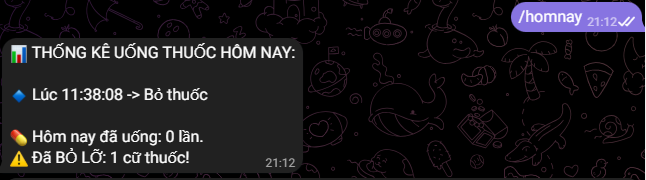
\includegraphics[width=\textwidth]{telegram_bot_get_daily.png}
    \caption{Giao diện truy vấn thống kê thời gian thực trên Telegram Bot}
    \label{fig:telegram_ui}
\end{figure}

\subsubsection{Cơ chế Báo cáo tự động định kỳ}

Trong các hệ thống thiết bị IoT chạy pin, việc duy trì kết nối mạng liên tục để canh đúng một mốc thời gian cố định trong ngày (ví dụ: 20h00) nhằm gửi báo cáo tổng kết là một sự lãng phí tài nguyên năng lượng rất lớn. Thậm chí, nếu tại thời điểm đó thiết bị mất điện hoặc rớt mạng, bản báo cáo sẽ không bao giờ được gửi đi. Để giải quyết triệt để vấn đề này, đề tài đã chuyển giao hoàn toàn tác vụ tổng hợp báo cáo cho hệ thống máy chủ đám mây thông qua tính năng Trình kích hoạt thời gian thực của Google Apps Script.

Cơ chế này hoạt động hoàn toàn độc lập với trạng thái (Online/Offline) của hộp thuốc phần cứng. Về mặt thuật toán, một hàm xử lý chuyên biệt (ví dụ: \texttt{sendDailySummary()}) được lập trình trên máy chủ với nhiệm vụ tự động quét toàn bộ cơ sở dữ liệu trong ngày, bóc tách và đếm số lượng các trạng thái "Đã uống", "Uống trễ", và "Bỏ thuốc". Sau đó, hàm sẽ định dạng các số liệu này thành một báo cáo hoàn chỉnh và gọi giao diện lập trình ứng dụng (API) của Telegram để đẩy tin nhắn về thiết bị di động của người quản lý.

Về mặt cấu hình triển khai, hệ thống sử dụng công cụ điều phối tác vụ nội bộ của Google. Trình kích hoạt được thiết lập với các thông số cấu hình tiêu chuẩn như sau:
\begin{itemize}
    \item \textbf{Nguồn sự kiện:} Dựa trên thời gian, đảm bảo máy chủ tự động đánh thức đoạn mã mà không cần bất kỳ tác động ngoại vi nào.
    \item \textbf{Loại trình kích hoạt:} Chu kỳ lặp lại theo ngày.
    \item \textbf{Khung thời gian thực thi:} Cấu hình trong khoảng 20:00 đến 21:00 (múi giờ GMT+7).
\end{itemize}

\begin{figure}[H]
    \centering
    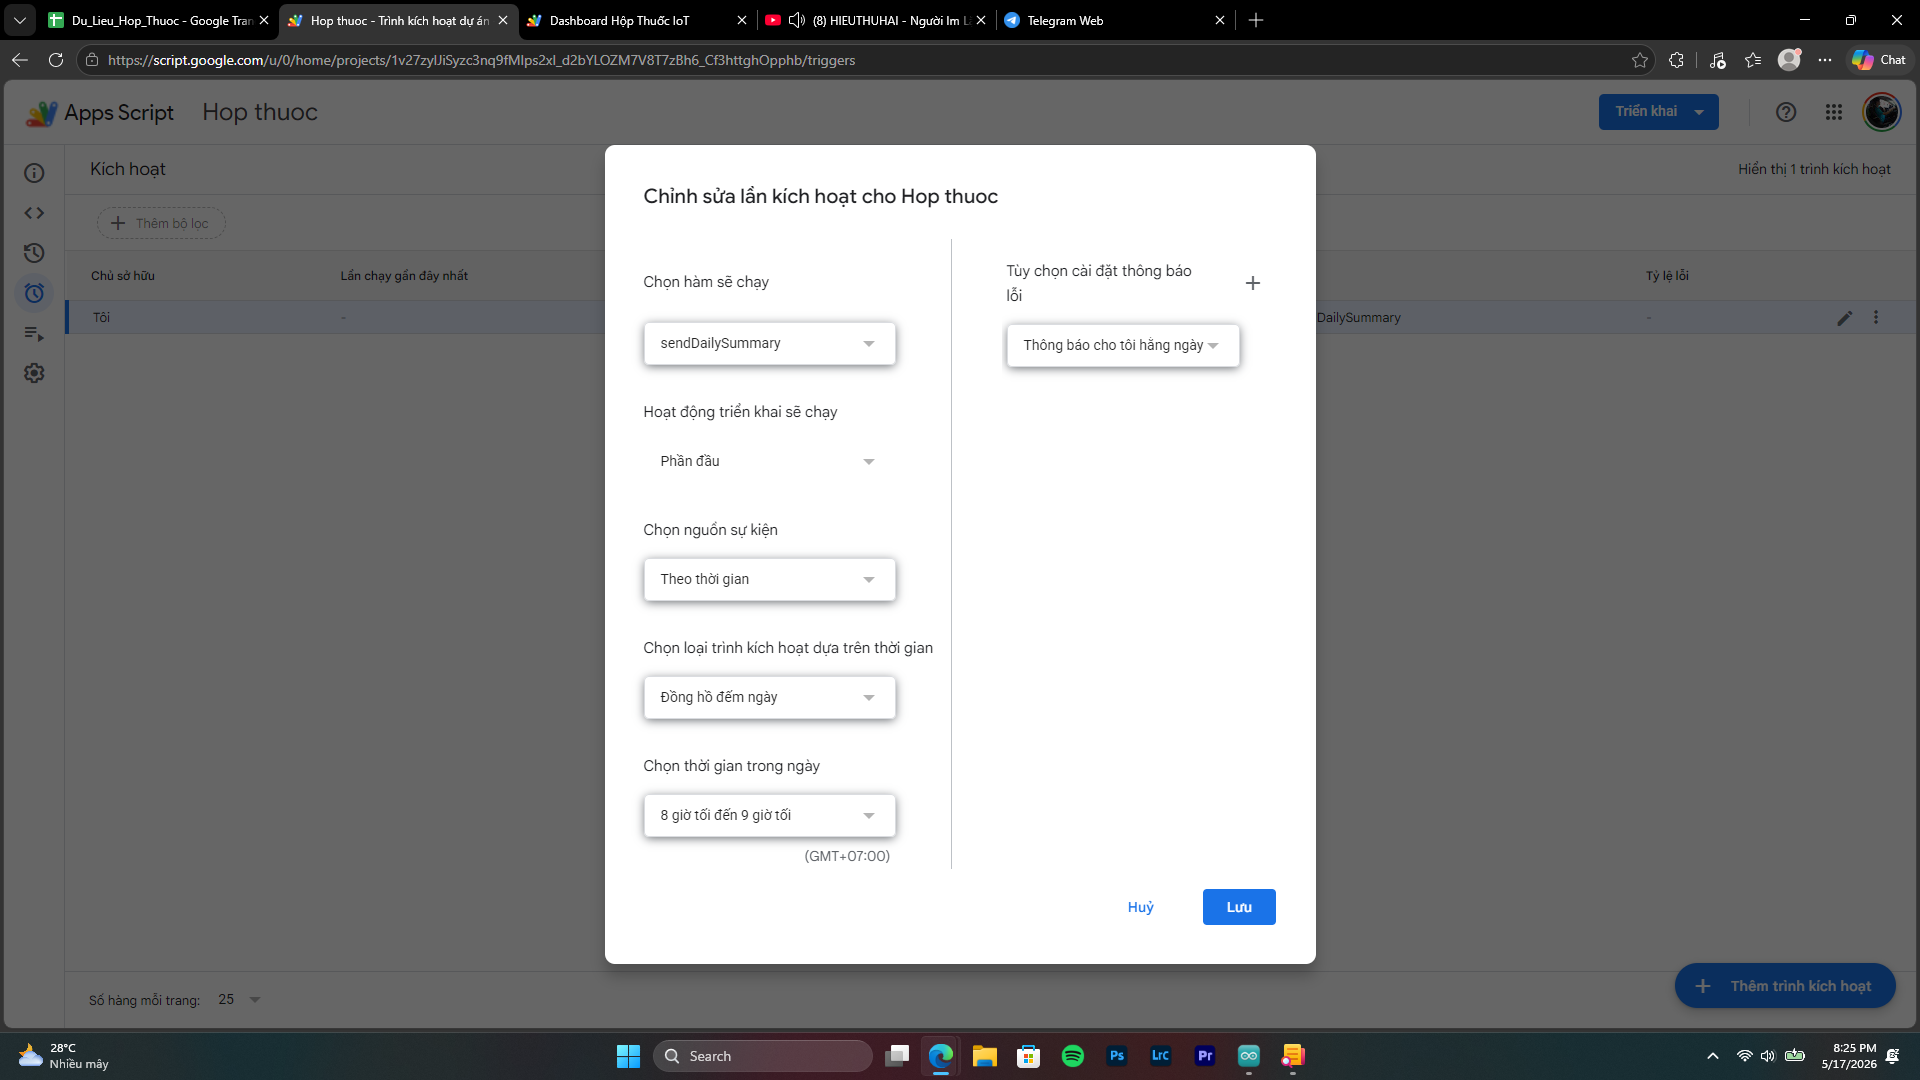
\includegraphics[width=\textwidth]{trigger_setup.png} % Thay tên file ảnh chụp màn hình cài đặt Trigger của bạn vào đây
    \caption{Giao diện cấu hình Trình kích hoạt thời gian trên hệ thống Google Apps Script}
    \label{fig:trigger_setup}
\end{figure}

Sự kết hợp giữa kịch bản lệnh trên máy chủ và trình kích hoạt tự động giúp hoàn thiện hệ sinh thái chăm sóc y tế khép kín. Người nhà bệnh nhân luôn nhận được bản tóm tắt tình hình tuân thủ phác đồ điều trị vào mỗi buổi tối một cách chính xác và ổn định nhất, tối ưu hóa triệt để vai trò của điện toán đám mây trong mô hình Internet vạn vật.


\subsection{Thiết kế Giao diện Quản lý trên nền Web}

Bên cạnh hệ thống cảnh báo qua tin nhắn Telegram, đề tài phát triển một trang quản trị chuyên dụng, phục vụ nhu cầu tra cứu và thiết lập phác đồ uống thuốc của bác sĩ hoặc người nhà. Trang mạng này được khởi tạo thông qua dịch vụ giao diện HTML của nền tảng máy chủ Google, giúp hệ thống không cần phụ thuộc vào dịch vụ lưu trữ bên thứ ba.

\subsubsection{Giao diện Giám sát theo Dòng thời gian}
Dựa trên tư vấn của giảng viên hướng dẫn, việc giám sát y tế yêu cầu cái nhìn tổng quan về "xu hướng tuân thủ" của bệnh nhân. Do đó, thay vì chỉ tra cứu dữ liệu đơn lẻ, trang quản trị được thiết kế chức năng tra cứu theo một khoảng thời gian (Từ ngày - Đến ngày).

Dữ liệu thô từ bảng tính được máy chủ phân tích, nhóm các sự kiện "Mở nắp" và "Đóng nắp" thành một cữ "Đã uống", sau đó thuật toán sẽ tự động sắp xếp theo trình tự thời gian tiến dần (từ cũ nhất đến mới nhất). Giao diện hiển thị được thiết kế theo dạng Dòng thời gian với các nhãn trạng thái trực quan:
\begin{itemize}
    \item \textbf{Màu xanh (Đã uống):} Xác nhận bệnh nhân đã tuân thủ đúng cữ thuốc.
    \item \textbf{Màu đỏ (Bỏ cữ):} Cảnh báo các cữ thuốc bị bỏ lỡ.
\end{itemize}

% GHI CHÚ: Chèn ảnh chụp trang web phần hiển thị dòng thời gian vào đây
\begin{figure}[H]
    \centering
    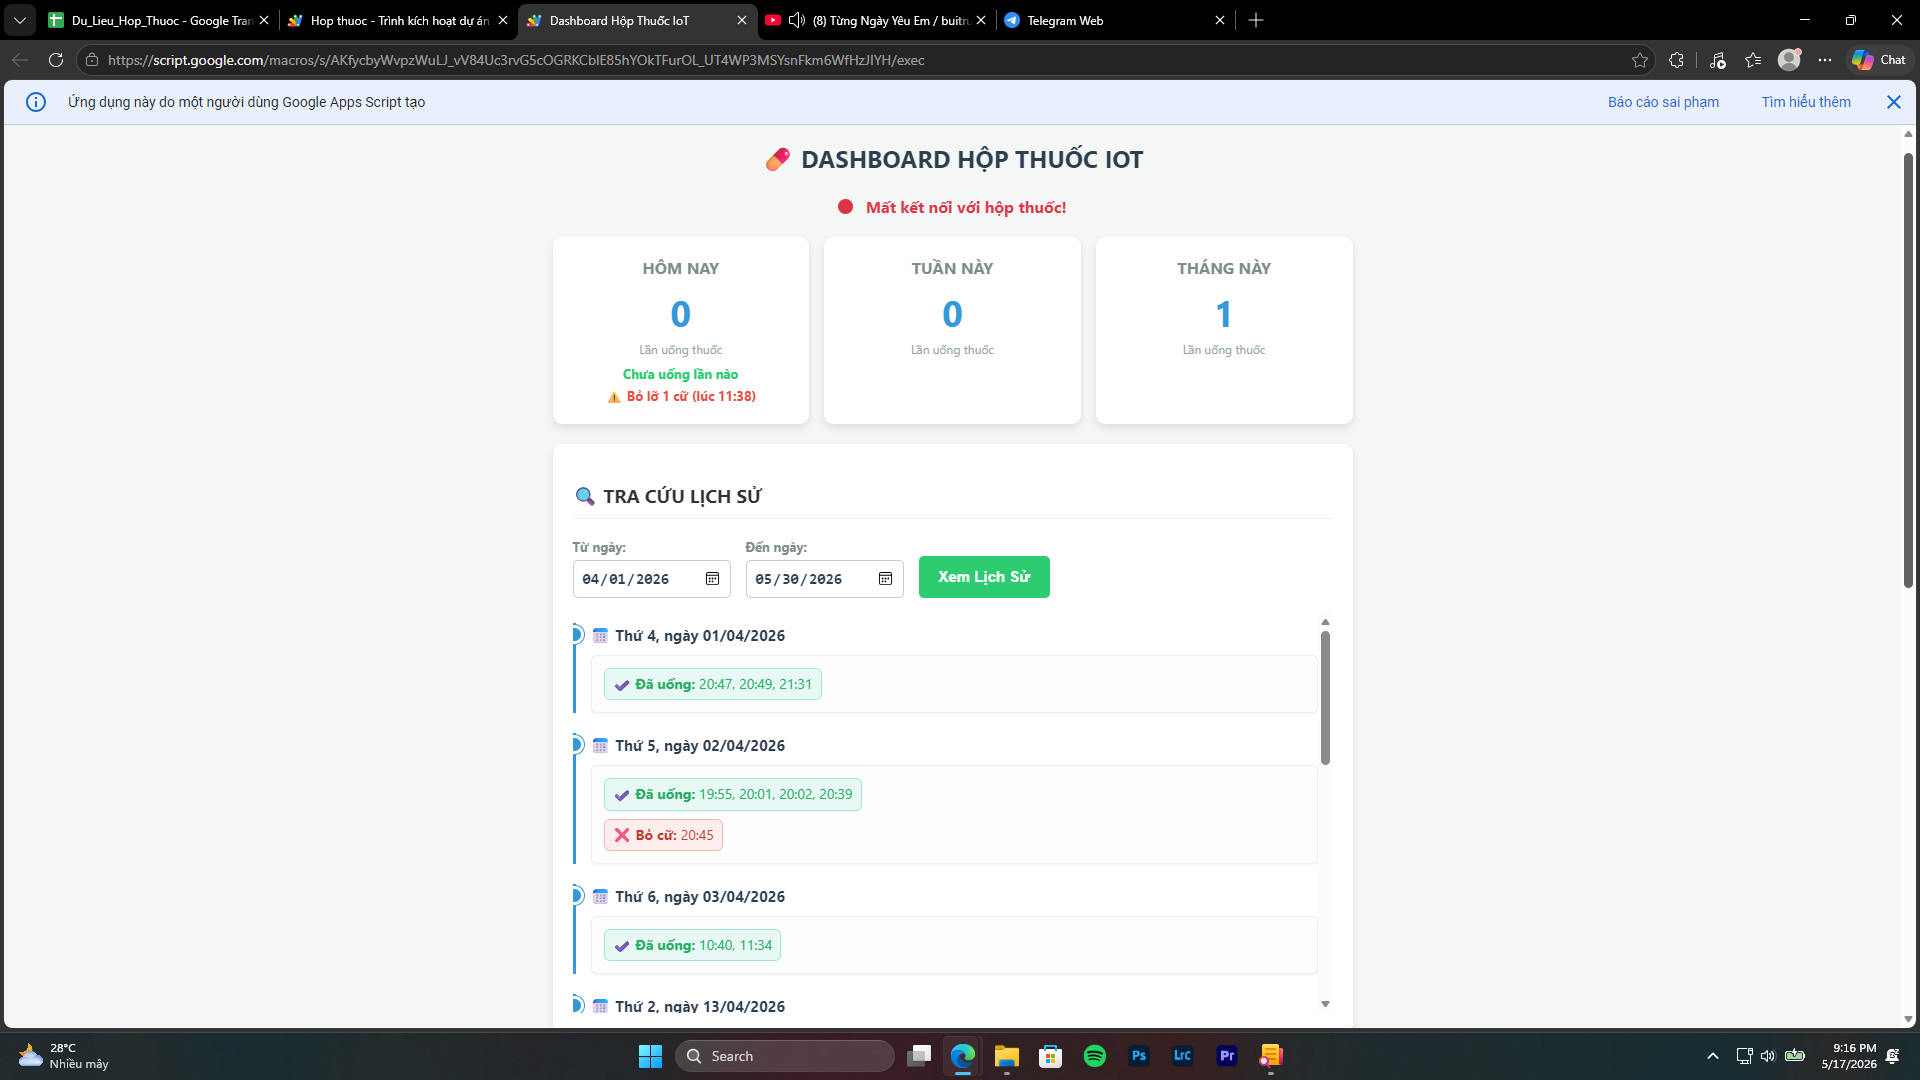
\includegraphics[width=\textwidth]{dashboard_timeline.png}
    \caption{Giao diện tra cứu lịch sử uống thuốc dạng Dòng thời gian}
    \label{fig:dashboard_timeline}
\end{figure}

\subsubsection{Giao diện Thiết lập Báo thức}
Trang quản trị cung cấp một phân hệ chuyên biệt cho phép bác sĩ điều trị hoặc người nhà thiết lập, tinh chỉnh và quản lý phác đồ uống thuốc của bệnh nhân từ xa. Giao diện được thiết kế trực quan với các thành phần chọn giờ chuẩn xác và bộ nút bấm cho phép tùy biến chu kỳ lặp lại theo từng ngày trong tuần.

Về mặt xử lý dữ liệu, khi người dùng hoàn tất thiết lập và ra lệnh lưu, trình duyệt web không gửi dữ liệu thô mà tiến hành tuần tự hóa toàn bộ danh sách báo thức thành một chuỗi ký tự được chuẩn hóa (ví dụ: \texttt{08:00|1234560,20:00|12345}). Kỹ thuật đóng gói dữ liệu này giúp tối ưu hóa không gian lưu trữ trên hệ thống máy chủ, khi toàn bộ phác đồ phức tạp chỉ chiếm dụng một ô nhớ duy nhất. Đồng thời, cấu trúc dữ liệu phân tách bằng các ký tự đặc biệt giúp vi điều khiển ESP32 dễ dàng tải về và bóc tách mảng thông tin bằng các hàm xử lý chuỗi cơ bản mà không làm tràn bộ nhớ vi mạch.

\begin{figure}[H]
    \centering
    % Bạn hãy cắt riêng khu vực "Cài đặt lịch uống thuốc" trên web (chỗ có các nút T2, T3, T4...) lưu thành file web_alarm.png để chèn vào đây nhé
    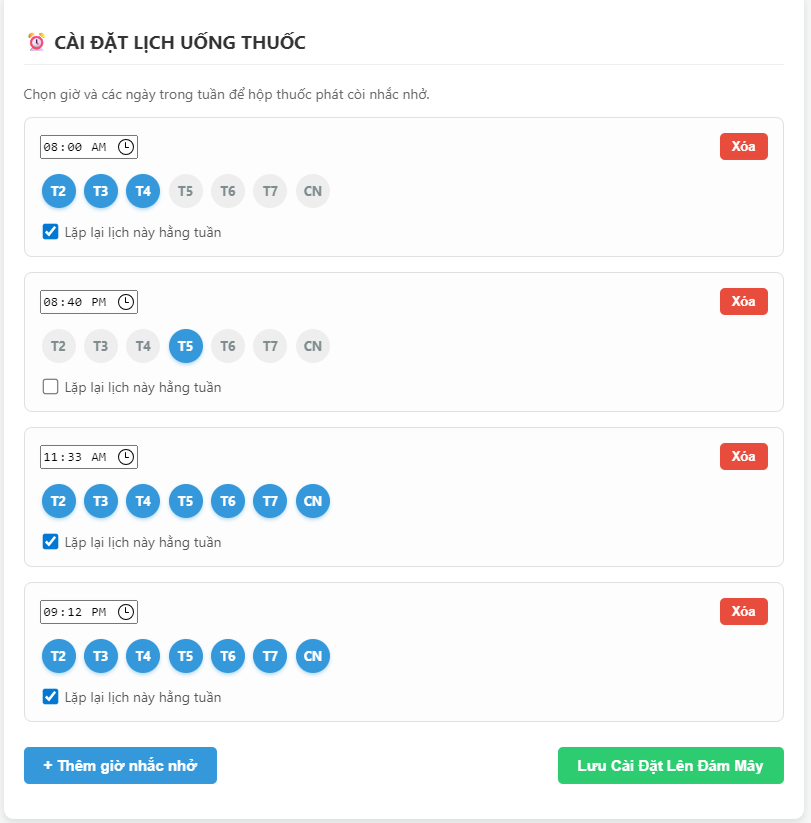
\includegraphics[width=0.85\textwidth]{web_alarm.png} 
    \caption{Phân hệ cài đặt phác đồ uống thuốc trực quan trên nền tảng Web}
    \label{fig:web_alarm}
\end{figure}

\subsubsection{Thiết kế Tương thích đa nền tảng và Tối ưu hóa truyền tải}
Để đảm bảo tính khả dụng trên đa dạng thiết bị đầu cuối từ máy tính cá nhân, máy tính bảng đến điện thoại di động, giao diện quản trị được xây dựng tuân thủ tiêu chuẩn thiết kế đáp ứng linh hoạt. Bằng việc áp dụng các thuộc tính dàn trang hiện đại của ngôn ngữ định dạng kiểu tĩnh, các khối thông tin thống kê tổng quan (Hôm nay, Tuần này, Tháng này) tự động sắp xếp dàn ngang trên màn hình lớn và tự động chuyển sang cấu trúc xếp chồng dọc khi kích thước khung nhìn thu hẹp, giúp nội dung không bị vỡ bố cục.

\begin{figure}[H]
    \centering
    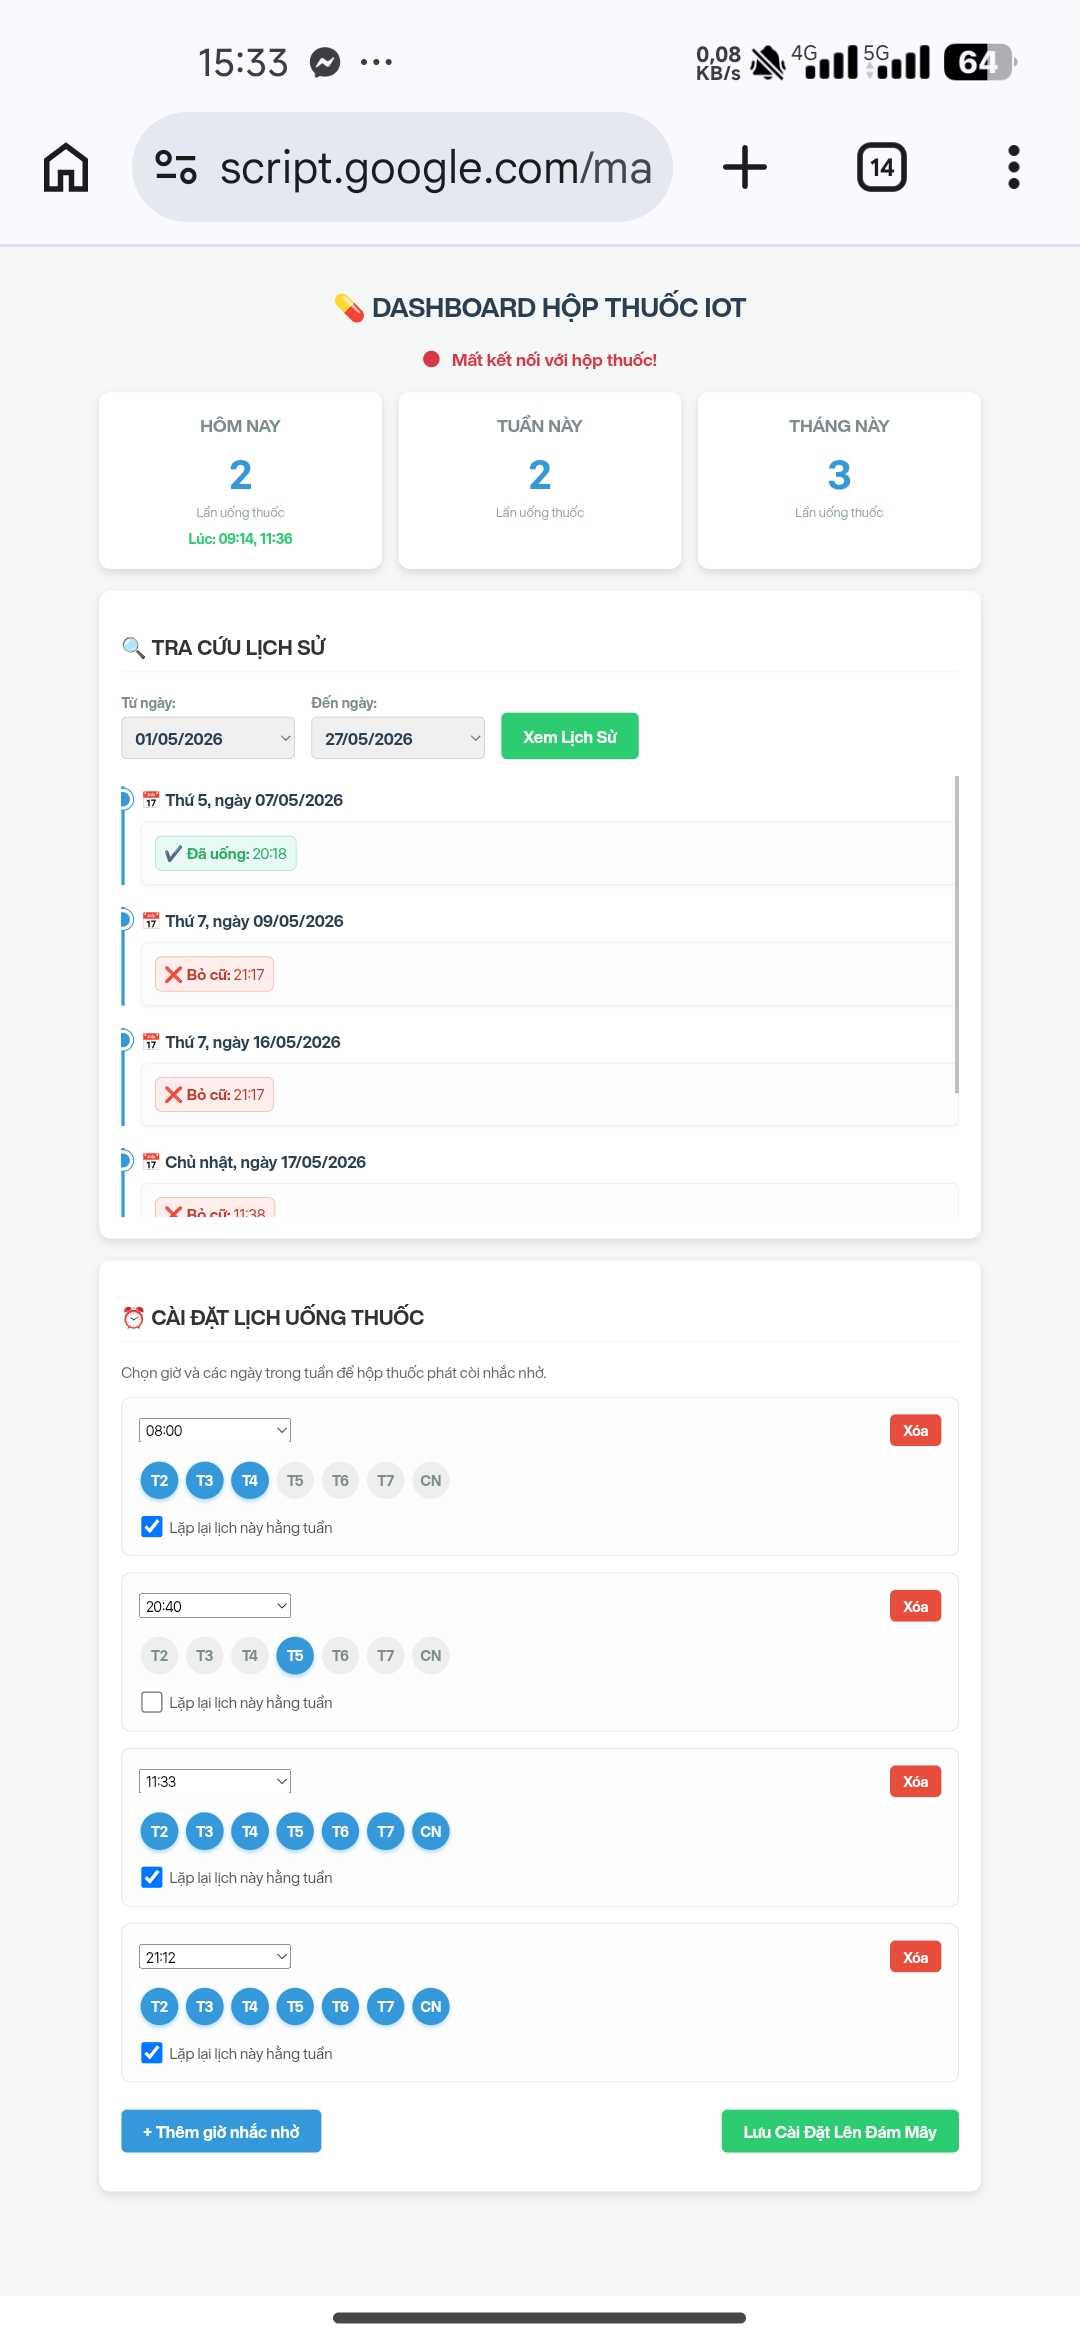
\includegraphics[width=0.48\textwidth]{giao_dien_smartphone.jpg} 
    \caption{Giao diện hiển thị thực tế của trang quản trị tự động tối ưu hóa và xếp chồng cấu trúc dọc trên màn hình điện thoại di động.}
    \label{fig:giao_dien_smartphone}
\end{figure}


Điểm đột phá của giao diện nằm ở việc ứng dụng kỹ thuật giao tiếp bất đồng bộ thông qua giao diện lập trình nội bộ của hệ sinh thái đám mây. Kỹ thuật này cho phép trang web trao đổi dữ liệu ngầm với máy chủ để cập nhật liên tục trạng thái hoạt động của thiết bị (Nhịp tim) hoặc tải bảng lịch sử uống thuốc mà không cần làm mới lại toàn bộ trang web. Kết quả truy vấn được luân chuyển và cập nhật trực tiếp vào cấu trúc phân cấp phần tử của giao diện, mang lại trải nghiệm tương tác mượt mà và tiết kiệm tối đa băng thông mạng.

\begin{figure}[H]
    \centering
    % Cắt riêng khu vực có cái chấm màu xanh lá cây "Thiết bị đang hoạt động" lưu thành file web_status.png
    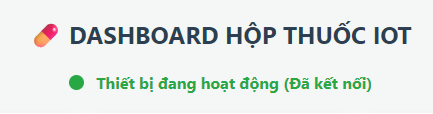
\includegraphics[width=0.6\textwidth]{web_status.png} 
    \caption{Cơ chế cập nhật trạng thái kết nối thiết bị bất đồng bộ theo thời gian thực}
    \label{fig:web_status}
\end{figure}

\subsubsection{Cơ chế bảo mật và Phân quyền truy cập}
Hệ thống thông tin y tế cá nhân đòi hỏi tiêu chuẩn bảo mật nghiêm ngặt nhằm bảo vệ tính riêng tư của người bệnh. Thay vì phải tự xây dựng các cơ chế mã hóa và quản lý phiên đăng nhập phức tạp, dễ phát sinh lỗ hổng bảo mật, đề tài tận dụng tối đa kiến trúc an ninh lớp ứng dụng của hệ sinh thái đám mây quản lý.

Trang web quản trị được triển khai dưới dạng một ứng dụng web nội bộ và kế thừa trực tiếp giao thức xác thực danh tính hai lớp. Quyền truy cập vào bảng điều khiển được kiểm soát chặt chẽ thông qua danh sách chia sẻ của tệp cơ sở dữ liệu. Cụ thể, chỉ những tài khoản thư điện tử được cấp quyền biên tập mới có khả năng truy xuất giao diện và can thiệp vào phác đồ điều trị. Mọi truy cập nặc danh hoặc từ các tài khoản không nằm trong danh sách trắng đều bị máy chủ từ chối phục vụ từ vòng ngoài, ngăn chặn hoàn toàn nguy cơ rò rỉ dữ liệu hoặc tấn công từ chối dịch vụ vào hệ thống.

\newpage
\begin{center}
    \section{KẾT QUẢ THỰC HIỆN}
\end{center}
%Nội dung chương 5

Sau thời gian nghiên cứu, thi công và lập trình, hệ thống "Hộp thuốc thông minh" đã được hoàn thiện. Để đánh giá tính khả thi và độ tin cậy của sản phẩm, hệ thống được đưa vào vận hành thực nghiệm thông qua các bài đo lường hiệu năng và các trường hợp kiểm thử khắt khe.

\subsection{Kết quả thi công phần cứng}
Quá trình thi công phần cứng được thực hiện tuần tự qua các giai đoạn: từ thử nghiệm kiểm chứng thuật toán trên testboard, thi công khối năng lượng, gia công mạch in thủ công cho đến khâu lắp ráp và cố định cơ khí. Kết quả cụ thể ở từng giai đoạn đều đáp ứng tốt các chỉ tiêu kỹ thuật đã đề ra.

\subsubsection{Kết quả thử nghiệm nguyên lý trên Testboard}
Trước khi tiến hành làm mạch in, toàn bộ linh kiện được lắp ráp thử nghiệm trên Testboard để kiểm chứng sơ đồ nguyên lý và sự tương thích của giao thức truyền thông. Kết quả cho thấy vi điều khiển ESP32 giao tiếp thành công với cả màn hình OLED và module đồng hồ DS3231 thông qua chung một bus I2C. Các lỗi nhiễu tín hiệu vật lý ban đầu đã được phát hiện và xử lý triệt để thông qua thuật toán chống dội phím (Debounce) cho công tắc hành trình.

\begin{figure}[H]
    \centering
    \includegraphics[width=0.75\textwidth]{ket_qua_testboard.jpg} % Bạn chèn ảnh chụp mạch cắm testboard vào đây
    \caption{Kết quả chạy thử nghiệm kiểm chứng nguyên lý và giao tiếp I2C trên Testboard}
    \label{fig:ket_qua_testboard}
\end{figure}

\subsubsection{Kết quả thi công mạch nguồn và hệ thống pin Li-Ion}
Hệ thống cấp nguồn di động đã được thi công hoàn thiện và hoạt động ổn định. Thay vì sử dụng các loại pin Polymer giá rẻ, đồ án đã tận dụng thành công cell pin Lithium-Ion tái chế từ điện thoại cũ (dung lượng $\sim 2000$ mAh), mang lại dòng xả cực kỳ ổn định và độ tin cậy hóa học cao.
\begin{itemize}
    \item \textbf{Mạch sạc và nâng áp:} Module J5019 hoạt động trơn tru, nạp tốt cho pin Li-Ion và kích điện áp lên mức 5V ổn định cấp cho hệ thống. Tụ hóa $100\mu F$ được bổ sung tại ngõ vào giúp dập hoàn toàn các xung sụt áp khi ESP32 bật sóng Wi-Fi.
    \item \textbf{Khối đo lường năng lượng:} Cầu phân áp gồm hai điện trở $100k\Omega$ mắc nối tiếp hoạt động chính xác. Điện áp pin được chia đôi và đưa vào chân D33 của bộ ADC1 trên ESP32. Kết quả đối chiếu với đồng hồ VOM cho thấy mạch đọc dữ liệu analog rất tuyến tính, sai số ở mức chấp nhận được và không gây hao hụt dung lượng pin nhờ nội trở cầu phân áp lớn.
\end{itemize}

\begin{figure}[H]
    \centering
    \includegraphics[width=0.8\textwidth]{ket_qua_nguon_pin.jpg} % Bạn chèn ảnh cụm mạch J5019 và cục pin vào đây
    \caption{Khối năng lượng sử dụng pin Li-Ion tái chế và module tích hợp J5019}
    \label{fig:ket_qua_nguon_pin}
\end{figure}

\subsubsection{Kết quả gia công mạch in (PCB) thủ công}
Mạch điện được gia công hoàn toàn bằng phương pháp ủi nhiệt và ăn mòn hóa học trong điều kiện phòng thí nghiệm. Nhờ việc thiết lập quy tắc thiết kế đi dây với độ rộng lớn (30-35 mil) và loại bỏ các góc gấp khúc 90 độ, kết quả phôi đồng sau khi ăn mòn đạt chất lượng rất tốt.
\begin{itemize}
    \item Các đường dẫn tín hiệu sắc nét, không xuất hiện tình trạng rỗ mạch hay đứt gãy đứt ngầm. 
    \item Các lỗi mối hàn ban đầu tại các chân rào cắm do diện tích tản nhiệt của bề mặt đồng quá lớn đã được khắc phục hoàn toàn bằng phương pháp gia nhiệt lại kết hợp nhựa thông lỏng, đảm bảo sự tiếp xúc điện tiêu chuẩn cho các module ngoại vi.
\end{itemize}

\begin{figure}[H]
    \centering
    \includegraphics[width=0.8\textwidth]{ket_qua_pcb.jpg} % Bạn chèn ảnh chụp bo mạch in vừa ủi/hàn xong (chưa lắp vào hộp) vào đây
    \caption{Bo mạch in một lớp hoàn thiện sau quá trình ăn mòn và hàn linh kiện}
    \label{fig:ket_qua_pcb}
\end{figure}

\subsubsection{Kết quả lắp ráp hoàn thiện sản phẩm}
Toàn bộ hệ thống mạch điều khiển, cơ cấu nguồn và các linh kiện ngoại vi được định vị và cố định chắc chắn vào bên trong không gian giới hạn của vỏ hộp cơ khí. Thiết kế đảm bảo sự liền mạch, thẩm mỹ và an toàn điện khi người dùng trực tiếp thao tác.
\begin{itemize}
    \item Màn hình OLED hiển thị rõ nét thời gian thực và ghi chú cữ thuốc với độ tương phản cao, hoạt động mượt mà với cơ chế giảm độ sáng (Dimming) tiết kiệm năng lượng.
    \item Còi báo động (Active Buzzer) phát tín hiệu âm thanh to, dứt khoát, đủ để thu hút sự chú ý của bệnh nhân lớn tuổi khi đến cữ.
    \item Công tắc hành trình phản hồi trạng thái cơ học vật lý chính xác. Các tác động đóng/mở nắp lập tức kích hoạt luồng cảnh báo ưu tiên trên màn hình mà không xảy ra bất kỳ sự cố treo hệ thống hay gửi sai lệch dữ liệu nào.
\end{itemize}

\begin{figure}[H]
    \centering
    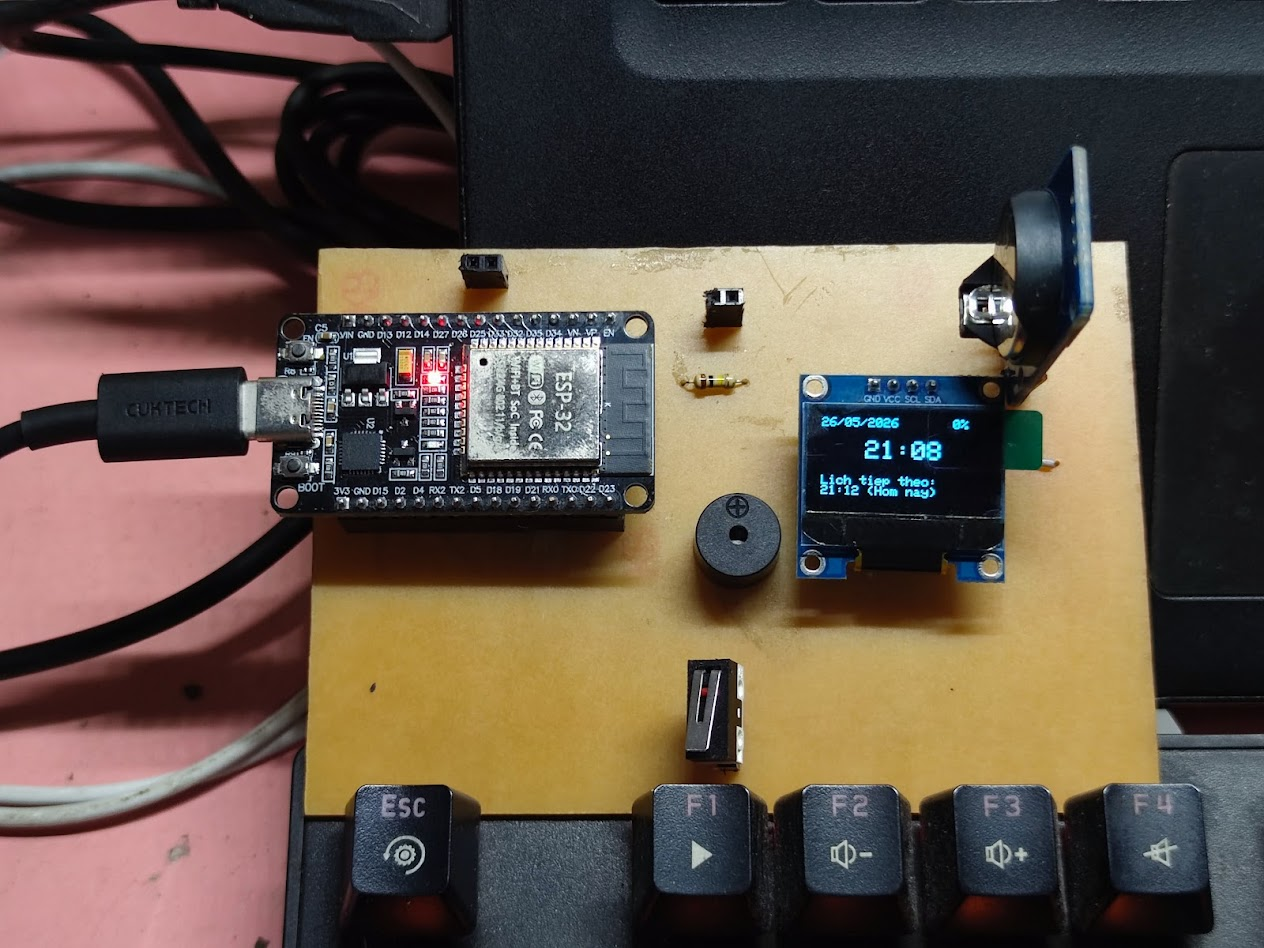
\includegraphics[width=0.75\textwidth]{mo_hinh_mat_truoc.jpg} % Chèn ảnh mặt trước (thấy màn hình)
    \caption{Hình ảnh thực tế mặt trước của Hộp thuốc thông minh sau khi lắp ráp hoàn thiện}
    \label{fig:mo_hinh_mat_truoc}
\end{figure}

\begin{figure}[H]
    \centering
    \includegraphics[width=0.75\textwidth]{mo_hinh_mat_sau.jpg} % Chèn ảnh mặt sau/bên trong/cơ khí
    \caption{Góc nhìn mặt sau thể hiện cấu trúc bố trí ngoại vi và hệ thống nắp hộp}
    \label{fig:mo_hinh_mat_sau}
\end{figure}

\subsection{Đánh giá thời gian đáp ứng và độ trễ truyền thông}
Một trong những thách thức lớn nhất của kiến trúc máy chủ phi tập trung là độ trễ khởi động ban đầu. Qua quá trình đo đạc thực tế bằng hàm đếm thời gian trên vi điều khiển, kết quả thời gian đáp ứng của hệ thống ghi nhận như sau:
\begin{itemize}
    \item \textbf{Thời gian thiết lập kết nối:} Mất trung bình $5.5 - 7.0$ giây để vi điều khiển thức dậy và hoàn tất quá trình bắt tay bảo mật mạng với máy chủ.
    \item \textbf{Độ trễ đẩy dữ liệu lên máy chủ:} Thời gian từ lúc mở nắp hộp đến khi dữ liệu được ghi nhận thành công trên bảng tính dao động từ $1.5- 3.5$ giây.
    \item \textbf{Độ trễ cảnh báo qua tin nhắn:} Tin nhắn đẩy về điện thoại người nhà gần như tức thời (dưới $5.0$ giây) kể từ khi hệ thống phát hiện vi phạm thời gian uống thuốc.
\end{itemize}
Nhìn chung, độ trễ tổng thể của hệ thống nằm trong ngưỡng dưới 10 giây, tuy không thực sự quá nhanh nhưng hoàn toàn đáp ứng được yêu cầu về thời gian thực cho một ứng dụng cảnh báo y tế.

\subsection{Kiểm thử các trường hợp vận hành thực tế}
Để đảm bảo hệ thống không bị lỗi xử lý logic trong quá trình sử dụng dài hạn, các trường hợp ngoại lệ cũng như thường xuyên đã được giả lập và kiểm thử thực tế.

\textbf{Trường hợp 1: Khởi tạo và cấu hình mạng lưới qua Cổng thông tin nội bộ (Captive Portal)}

Đối với các thiết bị IoT thương mại, việc nạp cứng thông tin mạng Wi-Fi vào mã nguồn là không khả thi. Để giải quyết bài toán này, hệ thống đã được tích hợp cơ chế quản lý cấu hình mạng động (WiFi Manager) cho phép người dùng tự thiết lập kết nối thông qua giao diện người dùng trên điện thoại thông minh.

\textbf{Cơ chế hoạt động thực tế:} 
Khi thiết bị được cấp nguồn lần đầu tiên, hoặc khi bộ định tuyến gia đình bị thay đổi mật khẩu, vi điều khiển ESP32 sẽ cố gắng kết nối mạng trong một khoảng thời gian chờ. Nếu thất bại, hệ thống tự động chuyển đổi từ chế độ Station sang chế độ Access Point. Lúc này, bộ phát sóng RF của ESP32 sẽ tạo ra một mạng Wi-Fi độc lập mang tên thiết bị (ví dụ: \texttt{Hop\_Thuoc\_IoT}). 

Khi người dùng sử dụng điện thoại thông minh kết nối vào mạng Wi-Fi này, hệ thống phân giải tên miền nội bộ của ESP32 sẽ lập tức đánh lừa các truy vấn web và tự động chuyển hướng màn hình điện thoại về một trang Captive Portal (Trang cổng thông tin cấu hình mạng). Tại giao diện này, vi điều khiển kích hoạt tính năng quét vô tuyến để liệt kê toàn bộ các mạng Wi-Fi khả dụng xung quanh. Người dùng chỉ việc chọn mạng và nhập mật khẩu. Chuỗi dữ liệu này lập tức được vi điều khiển ghi đè vào phân vùng nhớ tĩnh không bốc hơi của IC Flash. Sau đó, mạch tự động khởi động lại, tắt chế độ AP và kết nối thành công vào mạng Internet.

Kết quả kiểm thử cho thấy quá trình phát sóng AP và chuyển hướng người dùng diễn ra trơn tru. Giao diện cấu hình trực quan giúp người cao tuổi hoặc người nhà dễ dàng tái thiết lập kết nối mạng khi hộp thuốc được di chuyển sang vị trí địa lý khác mà không cần can thiệp phần cứng.

\begin{figure}[H]
    \centering
    % Hình 1: Điện thoại bắt sóng Wi-Fi của ESP32
    \begin{minipage}[b]{0.45\textwidth}
        \centering
        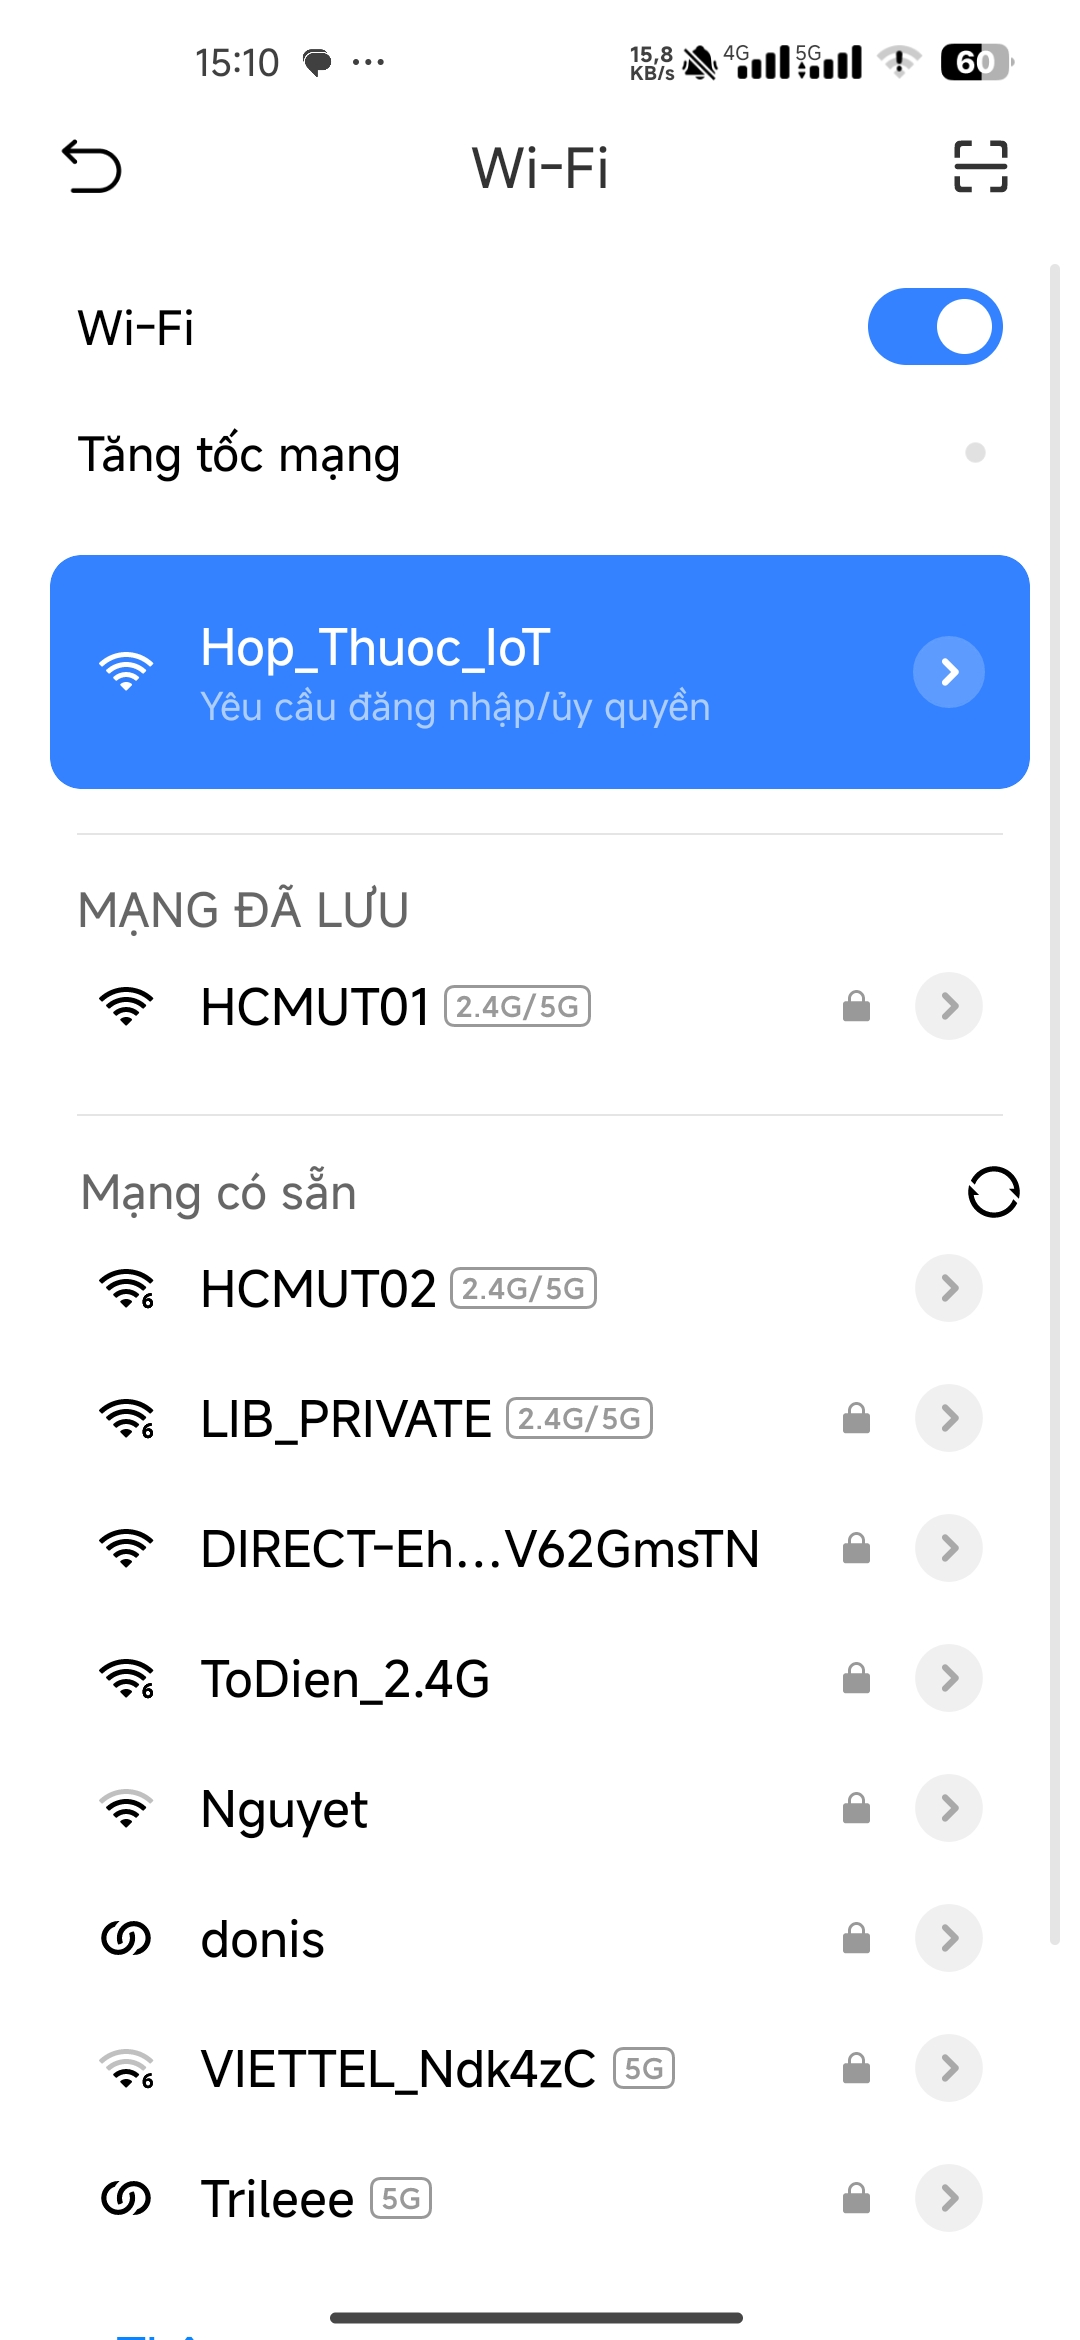
\includegraphics[width=0.85\textwidth]{wifi_scan.jpg} % Đổi tên file ảnh bắt sóng Wi-Fi của bạn vào đây
        \caption{Điện thoại tìm và kết nối vào mạng AP do mạch ESP32 phát ra}
        \label{fig:wifi_scan}
    \end{minipage}
    \hfill
    % Hình 2: Giao diện cấu hình WiFi Manager
    \begin{minipage}[b]{0.45\textwidth}
        \centering
        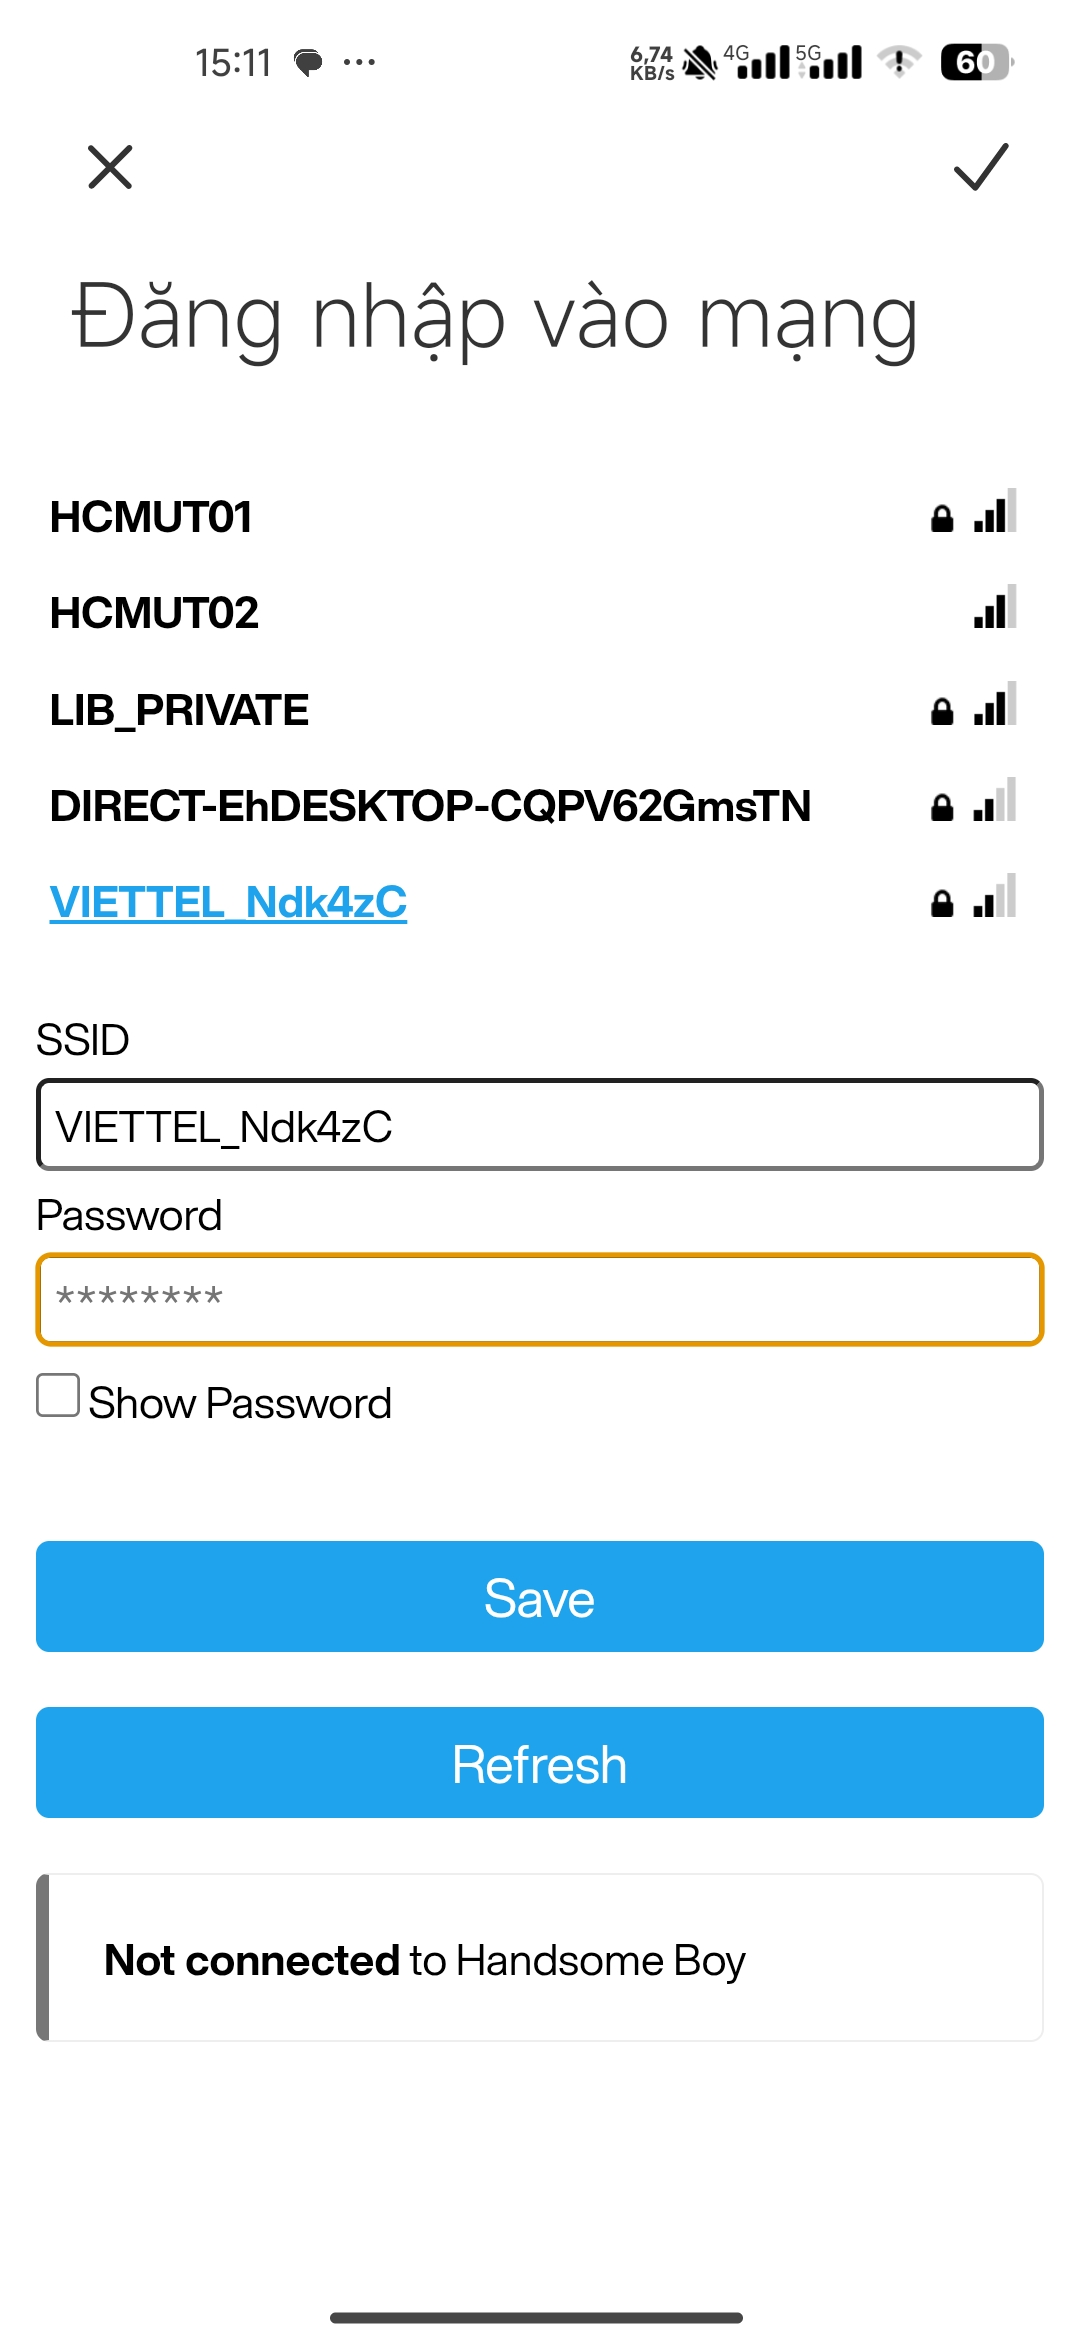
\includegraphics[width=0.85\textwidth]{wifi_manager.jpg} % Đổi tên file ảnh giao diện Web WiFi Manager của bạn vào đây
        \caption{Giao diện Captive Portal tự động hiện ra để cấu hình mạng}
        \label{fig:wifi_manager}
    \end{minipage}
\end{figure}

\textbf{Trường hợp 1: Kiểm thử chu trình nhắc nhở báo thức tiêu chuẩn}
Khi giá trị thời gian thực tế khớp với mốc lịch trình đã cài đặt trong mã nguồn, hệ thống kích hoạt chu trình nhắc nhở:
\begin{itemize}
    \item Khối hiển thị OLED hiển thị thông báo cữ thuốc trên màn hình.
    \item Còi báo động (Buzzer) phát ra âm thanh liên tục để thu hút sự chú ý của bệnh nhân.
\end{itemize}
Kết quả kiểm thử: Mạch phản hồi chính xác, không bị trễ giờ so với đồng hồ thực tế.

\textbf{Trường hợp 2: Mất kết nối mạng tại thời điểm báo thức} \\
Khi đến giờ uống thuốc nhưng hệ thống mất kết nối mạng nội bộ, thiết bị tự động chuyển sang chế độ hoạt động ngoại tuyến. Còi báo động vẫn phát ra chính xác dựa trên đồng hồ thời gian thực và danh sách báo thức đã được lưu trong bộ nhớ vĩnh cửu của vi điều khiển từ trước.

% GHI CHÚ: Chụp màn hình OLED lúc nó hiện thông báo mất Wi-Fi hoặc biểu tượng Offline
\begin{figure}[H]
    \centering
    \includegraphics[width=0.7\textwidth]{test_offline_oled.jpg}
    \caption{Màn hình hiển thị trạng thái hoạt động ngoại tuyến nhưng vẫn phát báo thức}
    \label{fig:test_offline}
\end{figure}

\textbf{Trường hợp 3: Bệnh nhân quên uống thuốc} \\
Khi quá thời gian chờ (5 phút) so với lịch trình mà hộp thuốc chưa được mở, hệ thống lập tức ghi nhận trạng thái "Bỏ thuốc" lên máy chủ cơ sở dữ liệu. Đồng thời, chương trình tự động gọi hàm gửi cảnh báo khẩn cấp dạng văn bản in đậm về ứng dụng Telegram của người quản lý.

% GHI CHÚ: Chụp màn hình điện thoại đoạn tin nhắn báo [!] CẢNH BÁO CHƯA UỐNG THUỐC
\begin{figure}[H]
    \centering
    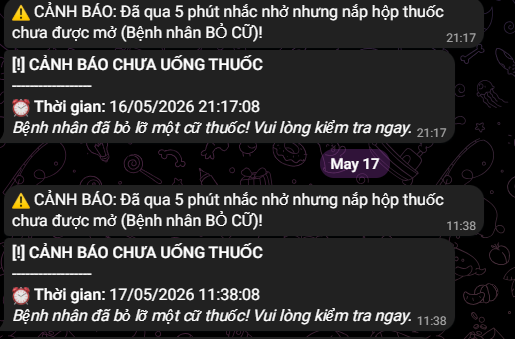
\includegraphics[width=0.75\textwidth]{test_bo_thuoc_tele.png}
    \caption{Tin nhắn cảnh báo khẩn cấp khi người bệnh bỏ cữ thuốc}
    \label{fig:test_bo_thuoc}
\end{figure}

\textbf{Trường hợp 4: Bệnh nhân uống bù thuốc sau khi bị bỏ lỡ} \\
Trường hợp bệnh nhân phát hiện quên và tiến hành mở hộp thuốc sau khoảng thời gian vi phạm (dưới 60 phút), hệ thống kích hoạt thuật toán lùi thời gian. Dòng trạng thái "Bỏ thuốc" trước đó trên máy chủ tự động được ghi đè thành "Uống trễ", đồng thời gửi cập nhật tình trạng mới về điện thoại. Trên trang quản trị, mốc thời gian uống bù cũng được cập nhật ngay lập tức.

% GHI CHÚ: Chụp màn hình Dòng thời gian trên Web hiển thị dòng chữ "Uống trễ"
\begin{figure}[H]
    \centering
    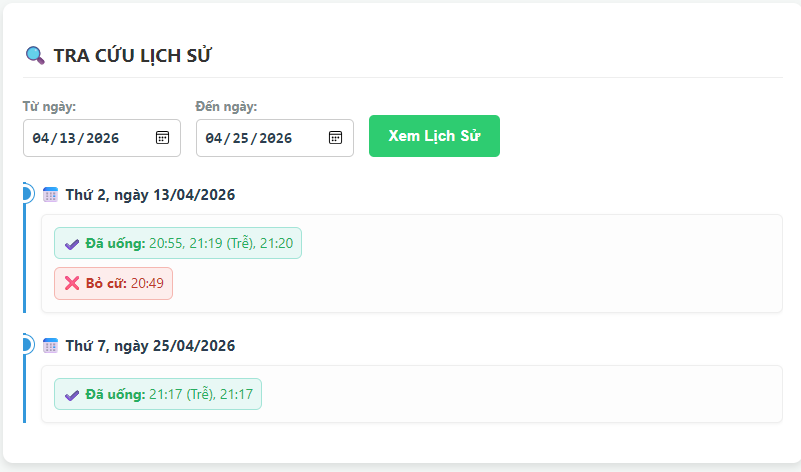
\includegraphics[width=0.9\textwidth]{test_uong_tre_web.png}
    \caption{Trang quản trị cập nhật lại trạng thái "Uống trễ" trên Dòng thời gian}
    \label{fig:test_uong_tre}
\end{figure}

\textbf{Trường hợp 5: Truy vấn thống kê từ xa} \\
Khi người quản lý gửi các tập lệnh truy vấn (ví dụ: lệnh lấy số liệu trong ngày) vào cửa sổ trò chuyện với bot tự động (Bot Telegram), hệ thống lập tức quét cơ sở dữ liệu và phản hồi lại bản tóm tắt số lần uống, thời gian uống cụ thể và số lần bỏ cữ.

% GHI CHÚ: Chụp màn hình lúc gõ lệnh /homnay và nhận được bảng thống kê
\begin{figure}[H]
    \centering
    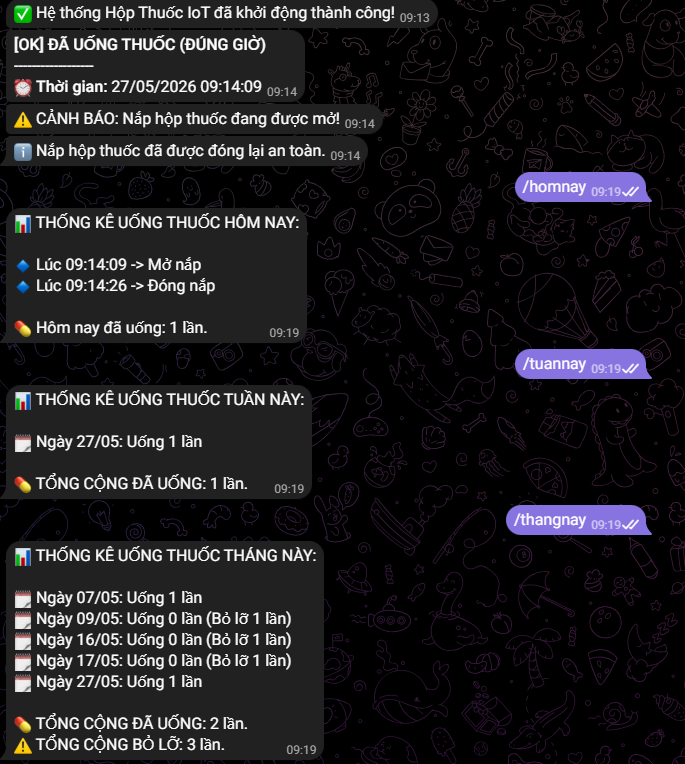
\includegraphics[width=0.75\textwidth]{test_truy_van_tele.png}
    \caption{Bot tự động phản hồi số liệu thống kê tuân thủ trong ngày, tuần, tháng khi người dùng nhập lệnh}
    \label{fig:test_truy_van}
\end{figure}

\textbf{Trường hợp 6: Tự động tổng hợp và báo cáo số liệu cuối ngày}

Nhằm tối ưu hóa quá trình giám sát mà không đòi hỏi người quản lý phải chủ động gửi tập lệnh truy vấn liên tục, hệ thống đã được tích hợp thêm tính năng báo cáo định kỳ tự động. Vào cuối mỗi ngày, cụ thể là trong khung giờ từ 20:00 đến 21:00 (theo giờ địa phương), máy chủ Google Apps Script sẽ tự động kích hoạt bộ lập lịch trình theo thời gian để thực hiện quét và trích xuất dữ liệu nhật ký lưu trữ trên Google Sheets.

Một bản báo cáo tóm tắt toàn diện bao gồm: tổng số cữ thuốc đã uống đúng giờ, số lần uống trễ và số cữ bị bỏ lỡ trong ngày hôm đó sẽ được hệ thống chủ động đóng gói và gửi dưới dạng tin nhắn thông báo trực tiếp về cửa sổ chat Telegram của người giám sát. Cơ chế chủ động này đảm bảo người nhà hoặc bác sĩ điều trị luôn nắm bắt được mức độ tuân thủ y lệnh của bệnh nhân một cách hệ thống theo ngày, kịp thời và liền mạch nhất.

\begin{figure}[H]
    \centering
    \includegraphics[width=0.75\textwidth]{bao_cao_cuoi_ngay.png} % Bạn chèn tên file ảnh chụp màn hình tin nhắn Telegram vào đây
    \caption{Bot tự động chủ động gửi bản tóm tắt thống kê tuân thủ điều trị vào cuối ngày}
    \label{fig:bao_cao_cuoi_ngay}
\end{figure}

\textbf{Trường hợp 7: Kiểm thử chu trình vận hành tiêu chuẩn (Người bệnh tuân thủ đúng giờ)}

Đây là kịch bản cốt lõi nhất của hệ thống, kiểm chứng sự phối hợp đồng bộ giữa khối thời gian thực, khối cảnh báo và cảm biến hành trình. Khi mốc thời gian thực tế khớp chính xác với cữ thuốc đã cài đặt, hệ thống lập tức kích hoạt chu trình nhắc nhở:
\begin{itemize}
    \item Khối hiển thị bừng sáng tối đa, cung cấp thông tin cữ thuốc rõ ràng trên nền giao diện tương phản cao.
    \item Còi báo động chủ động phát ra chuỗi âm thanh ngắt quãng tần số cao liên tục để thu hút sự chú ý.
    \item Ngay khi người bệnh thao tác mở nắp hộp để lấy thuốc (trong giới hạn 5 phút tiêu chuẩn), công tắc hành trình giải phóng tiếp điểm. Vi điều khiển lập tức ngắt còi báo động, chuyển trạng thái màn hình sang thông điệp cảm ơn và kích hoạt luồng dữ liệu mạng.
\end{itemize}

Kết quả ghi nhận trên hệ thống máy chủ cơ sở dữ liệu: Trạng thái đóng/mở nắp được cập nhật nối tiếp theo thời gian thực. Hệ thống tự động nhóm các thao tác này thành một sự kiện "Đã uống" hợp lệ và đồng bộ tín hiệu xanh lên giao diện giám sát dòng thời gian, xác nhận người bệnh đã tuân thủ hoàn toàn y lệnh.

\begin{figure}[H]
    \centering
    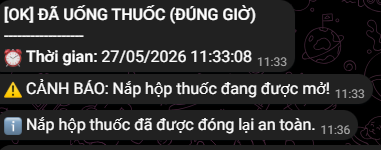
\includegraphics[width=0.5\textwidth]{test_uong_dung_gio1.png}
    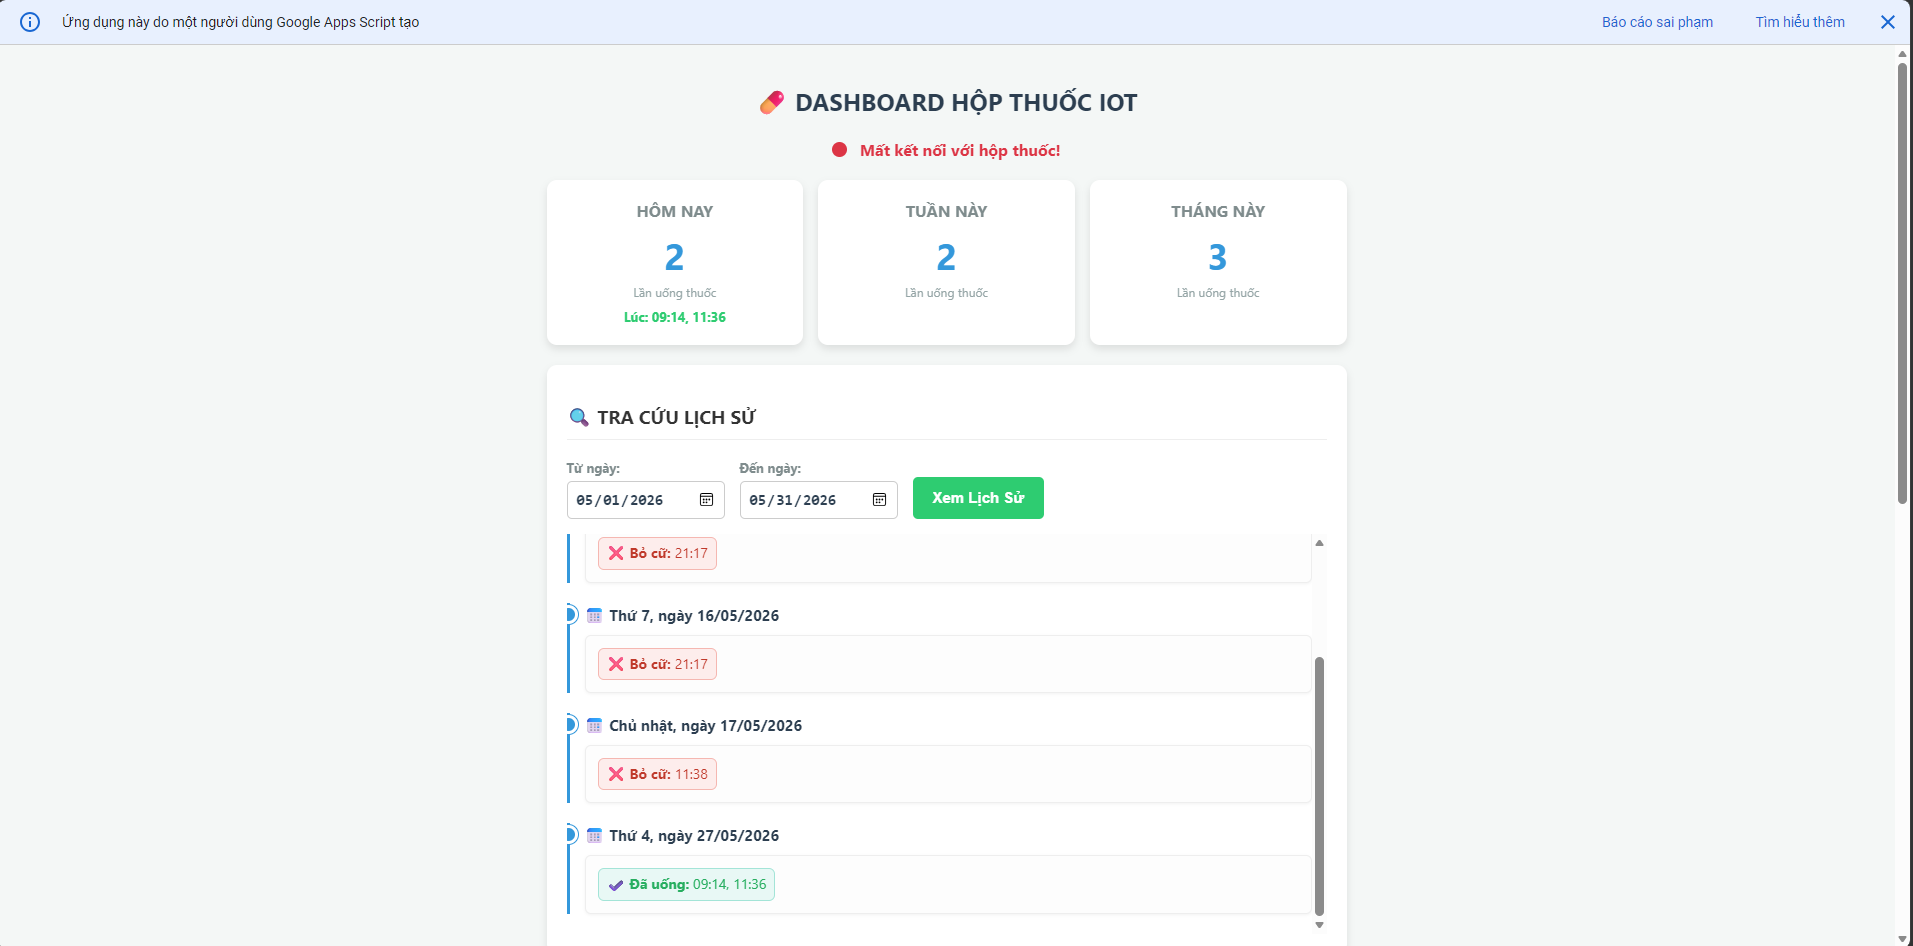
\includegraphics[width=\textwidth]{test_uong_dung_gio2.png}
    \caption{Hệ thống ghi nhận trạng thái tuân thủ y lệnh chính xác khi người bệnh thao tác đúng giờ}
    \label{fig:test_uong_dung_gio}
\end{figure}

\subsection{Đánh giá công suất tiêu thụ thực tế và phân tích sai số}

Bên cạnh các chỉ tiêu về chức năng, công suất tiêu thụ tĩnh của hệ thống là một tham số quan trọng quyết định tính khả thi khi vận hành bằng nguồn năng lượng di động. Theo tính toán lý thuyết khi áp dụng giải thuật điều chế độ sáng mờ tầng sâu cho màn hình hiển thị, dòng điện tiêu thụ kỳ vọng của toàn mạch sẽ ở mức cực thấp. Tuy nhiên, kết quả đo đạc thực nghiệm bằng thiết bị đo lường chuyên dụng cho thấy hệ thống duy trì mức công suất tiêu thụ sàn ổn định trong khoảng 0.3W đến 0.4W, tương đương dòng điện tổng rút ra từ nguồn 5V rơi vào khoảng 60mA đến 80mA.

\begin{figure}[H]
    \centering
    \includegraphics[width=0.75\textwidth]{do_cs_tt_typec.jpg}
    \caption{Hình ảnh thực tế phép đo công suất sàn bằng thiết bị đo USB chuyên dụng kết nối qua cổng Type C trên bo mạch ESP32.}
    \label{fig:do_cs_tt_typec}
\end{figure}

Sự chênh lệch giữa kỳ vọng lý thuyết của ngoại vi và thực tế hệ thống được phân tích và bóc tách dựa trên cấu trúc tổn hao năng lượng tĩnh của các thành phần phần cứng cốt lõi:

\begin{itemize}
    \item \textbf{Tổn hao duy trì kết nối vô tuyến:} Mặc dù vi điều khiển trung tâm ESP32 đã được hạ xung nhịp xử lý, nhưng bộ thu phát tín hiệu Wi-Fi nội tại bắt buộc phải duy trì trạng thái thức và giữ kết nối liên tục với bộ định tuyến để đảm bảo độ trễ đẩy thông báo cảnh báo tiệm cận mức số không. Trạng thái chờ kết nối mạng này chiếm dụng thường trực một dòng điện từ 30mA đến 40mA.
    \item \textbf{Dòng rò rỉ trên mạch ổn áp tuyến tính:} Nguyên mẫu phần cứng sử dụng bo mạch phát triển NodeMCU tích hợp sẵn vi mạch ổn áp hạ áp AMS1117. Bản thân vi mạch quản lý nguồn cấu trúc cũ này có dòng rò tĩnh từ 5mA đến 10mA dưới dạng nhiệt năng phân tán kể cả khi hệ thống không thực thi tác vụ nặng.
    \item \textbf{Tiêu hao từ linh kiện thụ động và chỉ thị trạng thái:} Tổ hợp đèn LED báo nguồn tích hợp trên bo mạch vi điều khiển và các điện trở phân áp luôn tiêu thụ một dòng điện tĩnh cố định khoảng 5mA.
    \item \textbf{Công suất phần dư của ngoại vi:} Khối hiển thị OLED sau khi bị ép xung giảm sáng bằng giải thuật phần mềm và khối thời gian thực DS3231 chỉ tiêu thụ tổng cộng chưa đến 5mA.
\end{itemize}

\textbf{Đánh giá tổng thể:} Mức công suất 0.3W đo đạc được thực chất là giới hạn đáy của phần cứng khi sử dụng bo mạch phát triển đa dụng kết hợp với yêu cầu duy trì kết nối mạng thời gian thực. Đối với một thiết bị y tế đòi hỏi tính khả dụng liên tục để gửi cảnh báo tức thời, mức tiêu thụ 60mA là một sự thỏa hiệp kỹ thuật xuất sắc giữa bài toán tiết kiệm năng lượng và độ tin cậy trong truyền thông cảnh báo.

\newpage
\begin{center}
    \section{KẾT LUẬN VÀ HƯỚNG PHÁT TRIỂN}
\end{center}

\subsection{Kết luận}
Đề tài \texttt{Thiết kế hộp thuốc thông minh IoT - IoT Smart Pillbox} đã hoàn thành xuất sắc các mục tiêu nghiên cứu và thi công thực tế được đề ra ban đầu. Quá trình thực hiện đồ án đã chứng minh tính khả thi của việc ứng dụng công nghệ Internet vạn vật vào việc hỗ trợ và giám sát tuân thủ y tế cá nhân. Cụ thể, đề tài đã đạt được những kết quả đáng chú ý sau:

\begin{itemize}
    \item \textbf{Về phần cứng:} Đã thiết kế và thi công thành công bo mạch điều khiển trung tâm dựa trên nền tảng vi điều khiển ESP32. Hệ thống hoạt động ổn định, tiết kiệm năng lượng nhờ sự phối hợp nhịp nhàng giữa mạch quản lý nguồn sạc, bộ đồng hồ thời gian thực độc lập và các ngoại vi hiển thị, cảnh báo. Cấu trúc mạch in được quy hoạch tối ưu, đáp ứng tiêu chuẩn của một thiết bị nhúng thu nhỏ.
    \item \textbf{Về phần mềm và truyền thông:} Hệ thống đã loại bỏ hoàn toàn sự phụ thuộc vào các dịch vụ lưu trữ trung gian tốn phí bằng cách xây dựng thành công kiến trúc máy chủ phi tập trung thông qua hệ sinh thái của Google. Các thuật toán xử lý đa nhiệm không đồng bộ trên vi điều khiển hoạt động mượt mà, kết hợp với cơ chế phản hồi theo thời gian thực qua rô-bốt tự động trên nền tảng nhắn tin. Đặc biệt, giải thuật xử lý ngoại tuyến và nhận diện hành vi uống trễ đã giải quyết triệt để các tình huống sai lệch dữ liệu trong thực tế.
\end{itemize}

Bên cạnh những kết quả đạt được, mô hình nghiên cứu hiện tại vẫn còn một số giới hạn nhất định. Về mặt cơ khí, thiết bị chưa có kết cấu phân chia nhiều ngăn thuốc độc lập cho các thời điểm khác nhau trong ngày. Về mặt cảm biến, công tắc hành trình mới chỉ xác nhận được thao tác mở nắp hộp, chưa thể khẳng định chắc chắn người bệnh đã thực sự lấy thuốc ra khỏi ngăn và uống hay chưa.

\subsection{Hướng phát triển và tiềm năng thương mại hóa}
Để đưa mô hình nghiên cứu tiến tới một sản phẩm công nghệ y tế (MedTech) hoàn thiện, đáp ứng các tiêu chuẩn khắt khe để thương mại hóa trên thị trường chăm sóc sức khỏe số, đề tài mở ra các định hướng nâng cấp chuyên sâu và toàn diện như sau:

\textbf{1. Tối ưu hóa cơ khí và Cảm biến y sinh đa tầng}
Phần vỏ hộp cần được thiết kế lại theo cơ cấu mâm xoay đa ngăn, tích hợp động cơ bước vi bước để tự động trích xuất đúng liều lượng thuốc cho từng thời điểm. Đi kèm với đó là việc trang bị cảm biến trọng lượng độ phân giải cao tại mỗi ngăn để đo lường chính xác lượng thuốc thay đổi, khắc phục điểm mù của công tắc hành trình hiện tại. Ngoài ra, việc tích hợp cảm biến môi trường (nhiệt độ, độ ẩm, ánh sáng) là bắt buộc để giám sát điều kiện bảo quản thuốc, đảm bảo dược tính không bị biến đổi trước khi đi vào cơ thể người bệnh.

\textbf{2. Tích hợp Thị giác máy tính tại biên}
Khai thác sức mạnh của các dòng vi xử lý lõi kép có hỗ trợ xử lý hình ảnh như ESP32-CAM hoặc dòng vi điều khiển AI chuyên dụng. Hệ thống sẽ được trang bị một camera góc rộng để chụp ảnh hoặc ghi hình khoảnh khắc người bệnh lấy thuốc. Thuật toán nhận diện khuôn mặt sẽ được thực thi trực tiếp trên thiết bị để xác thực danh tính, ngăn chặn tình trạng người nhà hoặc trẻ em uống nhầm thuốc.

\textbf{3. Tương tác Người - Máy bằng Trợ lý ảo giọng nói}
Tận dụng giao thức truyền âm thanh số (I2S) của ESP32 kết hợp với amply mini và micro định hướng, hộp thuốc có thể nâng cấp thành một loa thông minh. Bằng cách kết nối thông qua API với các mô hình ngôn ngữ lớn (LLMs), thiết bị có thể phát ra giọng nói tự nhiên để nhắc nhở, dặn dò cách uống (ví dụ: "Bà nhớ uống sau khi ăn no nhé") và cho phép người bệnh tương tác hỏi đáp về tác dụng phụ của thuốc ngay lập tức.

\textbf{4. Giao tiếp đa giao thức và Hệ sinh thái Smart Home}
Sản phẩm thương mại cần hỗ trợ các giao thức IoT tiêu chuẩn công nghiệp như MQTT, CoAP hoặc giao thức nhà thông minh Matter. Điều này cho phép hộp thuốc liên kết chéo với các thiết bị khác trong nhà, ví dụ: khi đến giờ uống thuốc, hệ thống sẽ tự động bật đèn phòng khách, phát thông báo lên loa Google Home, hoặc gửi tín hiệu SOS đến vòng đeo tay thông minh nếu phát hiện bệnh nhân bị ngã trong quá trình di chuyển đi lấy thuốc.

\textbf{5. Phân tích Big Data và Machine Learning}
Khi hệ thống được triển khai trên diện rộng, hàng triệu điểm dữ liệu về hành vi uống thuốc sẽ được thu thập về máy chủ. Các thuật toán Học máy sẽ phân tích để tìm ra sự tương quan giữa thời tiết, độ tuổi, loại bệnh với tỷ lệ bỏ cữ thuốc. Từ đó, hệ thống AI sẽ đóng vai trò dự đoán sớm rủi ro, đưa ra các cảnh báo tiên lượng để bác sĩ có thể điều chỉnh phác đồ kịp thời.

\textbf{6. Bảo mật dữ liệu và Quản lý năng lượng tái tạo}
Để đáp ứng tiêu chuẩn bảo mật y tế (như HIPAA), đường truyền dữ liệu cần được nâng cấp chuẩn mã hóa, đồng thời ứng dụng công nghệ Blockchain để lưu trữ log lịch sử uống thuốc, chống lại mọi sự can thiệp sửa đổi trái phép. Về mặt năng lượng, thiết bị có thể tích hợp thêm các tấm pin năng lượng mặt trời siêu nhỏ hoặc cuộn cảm sạc không dây, giúp thiết bị vận hành bền bỉ nhiều tháng mà không cần cắm sạc vật lý.

Những hướng phát triển này không chỉ định hình lại sản phẩm từ một thiết bị nhắc nhở đơn thuần trở thành một trạm y tế thu nhỏ, mà còn khẳng định giá trị cốt lõi của công nghệ IoT trong việc nâng cao chất lượng sống cho cộng đồng.

\newpage
\begin{center}
    \section{TÀI LIỆU THAM KHẢO}
\end{center}
%Nội dung chương 7
\renewcommand{\refname}{}
\renewcommand{\bibname}{}
\begin{thebibliography}{99}

% --- NHÓM DATASHEET LINH KIỆN ---

\bibitem{esp32_datasheet}
Espressif Systems, \emph{ESP32 Series Datasheet}, Version 4.3, 2023. [Trực tuyến]. Có tại: \url{https://www.espressif.com}.

\bibitem{esp32_trm}
Espressif Systems, \emph{ESP32 Technical Reference Manual}, Version 5.0, 2023.

\bibitem{ds3231_datasheet}
Maxim Integrated, \emph{DS3231 Extremely Accurate I2C-Integrated RTC/TCXO/Crystal}, Rev. 10, 2015.

\bibitem{ssd1306_datasheet}
Solomon Systech, \emph{SSD1306: 128 x 64 Dot Matrix OLED/PLED Segment/Common Driver with Controller}, Rev. 1.1, 2008.

\bibitem{tp4056_datasheet}
NanJing Top Power ASIC Corp., \emph{TP4056 1A Standalone Linear Li-lon Battery Charger with Thermal Regulation in SOP-8}, 2011.

\bibitem{mt3608_datasheet}
Aerosemi Technology, \emph{MT3608 High Efficiency 1.2MHz 2A Step Up Converter}, Rev. 1.2, 2014.

% --- NHÓM PHẦN MỀM VÀ NỀN TẢNG ---

\bibitem{gas_docs}
Google Developers, \emph{Google Apps Script Official Documentation}, 2024. \url{https://developers.google.com/apps-script}.

\bibitem{altium_docs}
Altium LLC, \emph{Altium Designer Documentation: PCB Design and Routing}, 2024. \url{https://www.altium.com/documentation}.

% --- NHÓM SÁCH CHUYÊN NGÀNH IOT ---

\bibitem{iot_book}
P. Waher, \emph{Learning Internet of Things}. Birmingham, UK: Packt Publishing, 2015.

\bibitem{kolban_esp32}
N. Kolban, \emph{Kolban's Book on ESP32}, 2018. \url{https://leanpub.com/kolban-ESP32}.

\end{thebibliography}

\newpage
    \section{PHỤ LỤC}
%Nội dung chương 8
\renewcommand{\refname}{}
\renewcommand{\bibname}{}
\begin{thebibliography}{99}
\bibitem{github_repo}
Project-IoT-Smart-Pillbox, \emph{Github Repository}, \url{https://github.com/thuanmazda/Project-IoT-Smart-Pillbox}

\bibitem{google_sheet_link}
Pillbox Cloud Data and Setting, \emph{Google Sheet Link}, \url{https://docs.google.com/spreadsheets/d/1F7vB3ncXRynr4YONkt-7NzRndev7CFtMYesXiH4w0Is/edit?usp=sharingx}

\bibitem{gas_web_dashboard}
Dashboard Web, \emph{Google Apps Script Web}, \url{https://script.google.com/macros/s/AKfycbyWvpzWuLJ_vV84Uc3rvG5cOGRKCblE85hYOkTFurOL_UT4WP3MSYsnFkm6WfHzJIYH/exec}

\end{thebibliography}

\begin{figure}[h]
    \centering
    
\includegraphics[width=0.4\textwidth]{qrcode.png}
    \label{fig:ma_qr_github}
    
\end{figure}

%\import{chap/}{chap0.tex}
\newpage
%\import{chap/}{chap1.tex}
%%%%%%%%%%%%%%%%%%%%%%%%%%%%%%%%%%%%%%%%%%%%%%%%%%%%%%%%%%%%%%
\newpage
%\import{chap/}{chap2.tex}
%%%%%%%%%%%%%%%%%%%%%%%%%%%%%%%%%%%%%%%%%%%%%%%%%%%%%%%%%%%%%%
\newpage
%\import{chap/}{chap3.tex}
%%%%%%%%%%%%%%%%%%%%%%%%%%%%%%%%%%%%%%%%%%%%%%%%%%%%%%%%%%%%%%
\newpage
%\import{chap/}{chap4.tex}
%%%%%%%%%%%%%%%%%%%%%%%%%%%%%%%%%%%%%%%%%%%%%%%%%%%%%%%%%%%%%%
\newpage
%\import{chap/}{chap5.tex}
%%%%%%%%%%%%%%%%%%%%%%%%%%%%%%%%%%%%%%%%%%%%%%%%%%%%%%%%%%%%%%
\newpage
%\import{chap/}{chap6.tex}
%%%%%%%%%%%%%%%%%%%%%%%%%%%%%%%%%%%%%%%%%%%%%%%%%%%%%%%%%%%%%%
%\newpage
%\import{chap/}{chap7.tex}
%%%%%%%%%%%%%%%%%%%%%%%%%%%%%%%%%%%%%%%%%%%%%%%%%%%%%%%%%%%%%%
\end{document}